\makeatletter
\def\@makechapterhead#1{%
  \vspace*{10\p@}%
  {\parindent \z@ \raggedleft \normalfont
    \ifnum \c@secnumdepth >\m@ne
      \if@mainmatter
        \LARGE\bfseries \@chapapp\space \thechapter
	\vskip 4pt
        \hrule height 2pt
        \par\nobreak
        \vskip 5\p@
      \fi
    \fi
    \interlinepenalty\@M
    \huge \bfseries #1\par\nobreak
\vskip 5pt

\hrule height 2pt   
 \vskip 10\p@  
  }}
\makeatother

\chapter{Semiconductor Diodes and Applications}\label{chap1}
\addtocontents{toc}{\protect\contentsline{chapter}{\protect Chapter \numberline{\thechapter.}
  Semiconductor Diodes and Applications}{\thepage--\pageref{1end}}}  

\medskip
\section{Introduction}\label{sec1.1}

An atom which is made up of electrons, protons and neutrons is the smallest distinguishable unit of different kinds of matter. Different atoms involve different arrangement of electrons, protons and neutrons. Each different atom represents a different element which is unique in its characteristics. Examples for elements are copper, silver, iron, silicon etc. Each of these elements contain only one kind of atom. An atom of silver differs from an atom of gold only in the number and arrangement of the neutrons, protons and electrons. The structure of the atom influences the electrical properties of a material.

Every element is composed of atoms and all of the atoms within a single element have the same structure. Each atom is composed of a central nucleus containing one or more positively charged particles called protons and neutrons. Charge of each proton is $1.6\times 10^{-19}$C and neutron has no charge. Around this nucleus electrons rotate continuously and the charge associated with each electron is $-1.6\times 10^{-19}$C. Since the positive charge on each proton is equal in magnitude to the negative charge on each electron, the complete atom is electrically {\em neutral} because they are equal in numbers. The mass of the electron is approximately $9.11\times 10^{-31}$ kg. Protons have mass about 2000 times of the mass of electrons.

Electrons rotate around the nucleus of their atoms in specific energy levels. Energy is required to move electrons away from the nucleus. Thus, electrons closest to the nucleus have less energy than those away from the nucleus. This is shown in Fig.~\ref{fig1.1}. As the electron is given more and more energy it moves farther and farther away from the nucleus. When this energy becomes large enough to move it completely out of the field of influence of the atom, the atom is said to be {\em ionized}. An atom that has more or fewer electrons than its normal number is said to be ionized. If an atom loses electrons, it becomes {\em positive ion} and if it gains electrons, it becomes {\em negative ion}.

Energy associated with the electron in each specific energy level is measured in terms of electron volts (eV), where one electron volt is the energy required to move an electron across a potential difference of one volt.
$$
1\text{~eV}=1.6\times 10^{-19}\text{~~Joules}
$$
\begin{figure}[H]
\centering
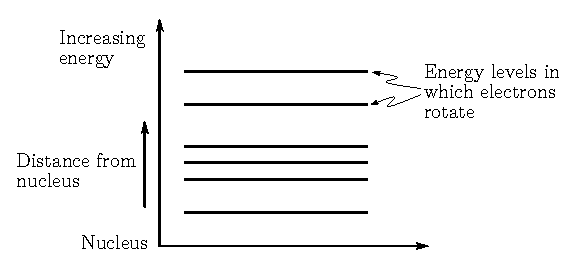
\includegraphics{chap1/fig1.1.eps}
\caption{Discrete energy levels of an atom}\label{fig1.1}
\end{figure}

Substances are formed by the bonding of atoms. When atoms are bonded, the individual energy levels of electrons of every atom merge each other to form energy bands of allowable energy states. The gap between the energy bands are called forbidden energy gap in which no electron can exist. Exciting an atom, i.e., adding energy to an atom may result in electrons overcoming the forbidden energy gap and moving into the higher level energy band.

The outermost energy band of an unexcited atom is the {\em valance band}. If energy is provided to the atoms in the valance band, electrons may jump to the conduction band. Once the electrons reach the conduction band, they are relatively free and can move about the material without being associated with any particular atom.

Fig.~\ref{fig1.2} shows the valance and conduction bands which are separated by forbidden energy gap.
\begin{figure}[H]
\centering
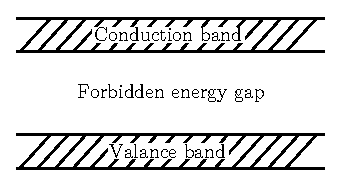
\includegraphics{chap1/fig1.2.eps}
\caption{Different energy bands of a substance}\label{fig1.2}
\end{figure}

\subsection{Classification of materials}\label{sec1.1.1}

The energy gap between valance and conduction band is an important measure of how materials behave electrically. Depending on the structure of the energy band, materials can be classified into three categories.

(i) insulators\qquad (ii) semi-conductors\qquad (iii) conductors

\heading{Insulators~:} These materials are characterized by a wide forbidden energy gap. This implies that valance electrons cannot be boosted to the conduction band unless relatively a large amount of energy is applied. Since the forbidden energy gap is very large, the applied field will not provide sufficient energy to the electrons to jump from the valance band to the conduction band. Therefore in an insulator conduction is very poor. Few good examples for insulators are diamond, wood, etc. The width of the forbidden energy gap $\rmE_{\rmG}$ is around 6 eV.

\heading{Semiconductors~:} A substance in which the width of the forbidden energy gap is relatively small ($\rmE_{\rmG}$ = 1 eV) is called {\em semiconductor}. Although several different materials behave as semiconductors, there are two which have found the greatest applications. They are silicon (Si) and germanium (Ge), both of which have four valance electrons. The width of the forbidden energy gap $\rmE_{\rmG}$ of Si and Ge are 1.21 eV and 0.785 eV respectively at $0^{\circ}$ K. (absolute zero temperature). This much of energy cannot be provided from an external applied field. Thus at $0^{\circ}$ K, valance band is full and the conduction band is empty and these materials behave as insulators.

But as temperature is increased, some of the valance electrons acquire sufficient thermal energy greater than $\rmE_{\rmG}$ and move into the conduction band. Once they reach the conduction band, they can move about under the influence of even a small applied field because they are not attached to any atoms. The electrons in the conduction band are known as {\em free electrons}. The absence of an electron in the valance band is shown by a small circle in Fig.~\ref{fig1.3} and is called {\em holes}. These holes may serve as a carrier of electricity comparable with the free electrons. Semiconductor in this pure form is known as {\em intrinsic semiconductor}.
\begin{figure}[H]
\centering
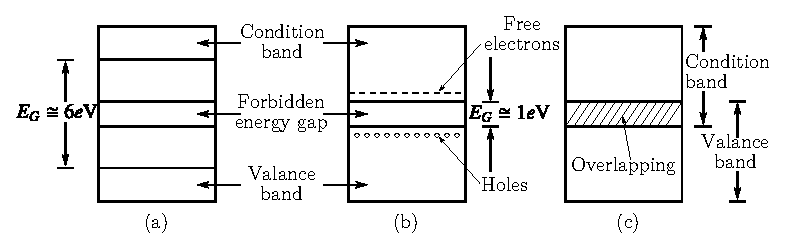
\includegraphics[scale=1.05]{chap1/fig1.3.eps}
\caption{Energy band diagram of (a) an insulator\\ (b) a semi conductor and (c) a conductor}\label{fig1.3}
\end{figure}

\smallskip
The four valance electrons associated with each Si or Ge atom form the pairs of electrons with neighbouring atoms as shown in Fig.~\ref{fig1.4}. Thus, there results a binding force between neighbour atoms. This electron pair or covalent bond is represented by two dashed lines connecting each atom to its neighbours.
\begin{figure}[H]
\centering
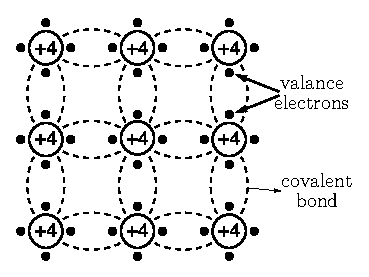
\includegraphics{chap1/fig1.4.eps}
\caption{Two dimensional representation of covalent-bond structure for Si and Ge}\label{fig1.4}
\end{figure}

If enough energy is supplied to these covalent bonds, they would be broken and the electrons would move to the conduction band, where they would be free to carry an electric current. Thus, as the temperature is increased, more number of covalent bonds are broken, thereby resulting in more free electrons in the conduction band and holes in the valance band which increases the conductivity of the material. Thus, semiconductor has {\em negative temperature coefficient of resistance}.

\heading{Conductor~:} Elements in which valance band and conduction band overlap each other are called {\em conductors} or {\em metals}. Although the number of electrons in the conduction band in a conductor increases with temperature, their number becomes so vast that they collide frequently and interfere with each other's progress when under the influence of an applied electric potential. Therefore, it becomes more difficult to establish an uniform flow of charge at higher temperature, which results in {\em positive temperature coefficient of resistance} for conductors. In conductors current is due to free electrons only.

\section{Electrons and holes in an Intrinsic Semiconductor}\label{sec1.2}

The conductivity of any material is proportional to the concentration of free electrons n. For a good conductor, n is very large (1028 electrons/m$^{3}$) and for an insulator, n is very small ($\cong$ 107 electrons/m$^{3}$) and for a semiconductor n lies between these two values. The valance electrons in a conductor are free to move as they are readily available in large numbers in the conduction band (because balance band and conduction band overlap), even at low temperature. But in an intrinsic semiconductor (i.e., pure semiconductor) the valance electrons are not free to wander but rather are trapped in a covalent bond between two adjacent atoms as shown in Fig.~\ref{fig1.6}. Examples for widely used semiconductors are silicon (Si) and germanium (Ge).

At very low temperature (approximately absolute zero temperature i.e. at $0^{\circ}$ K), the crystal structure of an intrinsic semiconductor is as shown in Fig.~\ref{fig1.6} and they behave as an insulator because no free carriers of an electricity are available.

At room temperature, some of the covalent bonds get broken because of the thermal energy supplied to the crystal and conduction becomes possible. This is shown in Fig.~\ref{fig1.7}. Here an electron which ordinarily (at very low temperature) forms part of a covalent bond is shown dislodged and thus free to move about in a random fashion within the crystal.
\begin{figure}[H]
\centering
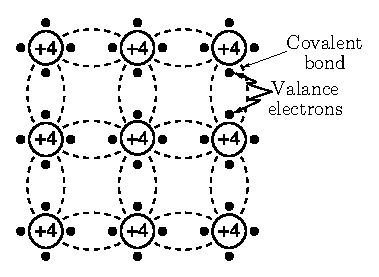
\includegraphics{chap1/fig1.6.eps}
\caption{Two dimensional crystal structure of intrinsic semiconductor}\label{fig1.6}
\end{figure}

\begin{figure}[H]
\centering
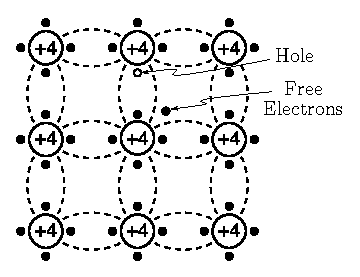
\includegraphics{chap1/fig1.7.eps}
\caption{Two dimensional crystal structure of an intrinsic semiconductor with a broken covalent bond at room temperature}\label{fig1.7}
\end{figure}

The amount of energy required to break a covalent is about 0.72 eV for Ge and 1.1 eV for Si at room temperature. The additional energy required for breaking a covalent bond may be supplied (i) by raising the temperature and thereby providing the thermal energy (ii) by incidence of photons in the visible range.

When an electron has broken away from a covalent bond, the vacancy left behind in the crystal structure is called a hole and is represented by a small circle as shown in Fig.~\ref{fig1.7}. This hole also serve as a carrier of electricity in the same way as the free electrons. A free electron and hole has some magnitude of charge i.e., $1.6\times 10^{-19}$C.

\vskip .1cm
Fig.~\ref{fig1.8} illustrates the movement of hole in a semiconductor.

\vskip .1cm
Consider a hole is existing as A. Suppose that a valance electron at B manages to move into the hole at A. In this case recombination takes place and hole at A has been neutralized. However, this results in a vacancy for an electron at B. We can say either that the valance electron moved to fill the hole or that the hole moved to where the valance electron used to be.
\begin{figure}[H]
\centering
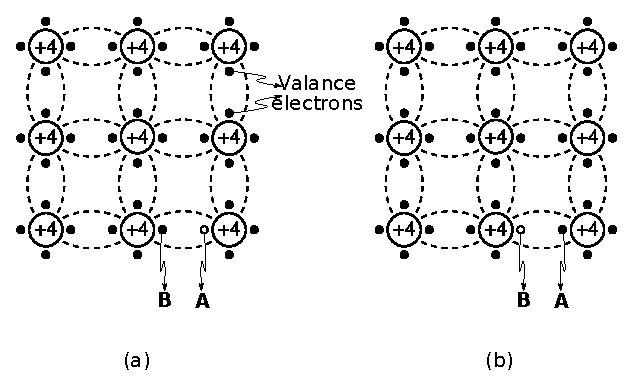
\includegraphics[scale=1.1]{chap1/fig1.8.eps}
\caption{(a) A missing valance electron at A represent a hole\\ (b) Valance electron from B moves into the hole A, equivalently hole from A to B}\label{fig1.8}
\end{figure}

\vskip .1cm
The free electrons in the conduction band are not under the influence of any atom, thus, it can move freely, when an electric field is applied. But for holes, the situation is different. Their energy level is not sufficient to place them in the conduction band, but they can move into nearby holes. Thus, their motion is more restricted than the free electrons in the conduction band. Hence the mobility of free electron is greater than that of holes.

\vskip .15cm
At $300^{\circ}$K the mobility of free electron in Ge is 0.38 m$^{2}$/V.s. and that of hole is 0.18 m$^{2}$/V.s. Similarly, the mobility of free electron in Si is 0.13 m$^{2}$/V.s. and that of hole is 0.05 m$^{2}$/V.s.

\vskip .15cm
Since holes in an intrinsic semiconductor are created by electrons that have been freed from the breakage of covalent bonds, the number of free electrons must be equal to the number of holes. Thus, in an intrinsic semiconductor, the electron density (electrons/m$^{3}$) equals the hole density (holes/m$^{3}$).
\begin{equation}
\text{i.e.,}\quad \rmn_{\rmi}=\rmp_{\rmi}\label{eq1.1}
\end{equation}
\begin{tabbing}
where \= n$_{\rmi}$ = intrinsic electron density (electron/m$^{3}$)\\[4pt]
      \> p$_{\rmi}$ = intrinsic hole density (hole/m$^{3}$)
\end{tabbing}

\vskip .1cm
In Eqn.~\eqref{eq1.1}, $\rmn_{\rmi} = \rmp_{\rmi}$ is also known as {\em intrinsic concentration}.

\vskip .1cm
At room temperature (i.e., at $300^{\circ}$ K), the intrinsic concentration for Ge and Si is approximately equal to $2.5\times 10^{19}$ carriers/m$^{3}$ and $1.5\times 10^{16}$ carriers/m$^{3}$ respectively. 

\vskip .1cm
The intrinsic concentration increases by approximately 5.5\%\ per degree rise in temperature. Thus the conductivity also increases approximately by 5.5\%\ per degree rise in temperature.

\vskip .1cm
When an electric potential is applied across an intrinsic semiconductor, the electric field established in the material causes free electrons to drift in one direction and holes to drift in the other. Because the positive holes move in the opposite direction of the negative electrons flow, these two components of current add, rather than cancel. This total current, due to the applied electric field, is called {\em drift current}.

\vskip .1cm
The drift current depends on many factors, such as the mobility $\mu$ of charge carriers, the kind of materials etc. Typical values for hole mobility $\mu_{\rmp}$ and electron mobility $\mu_{\rmn}$ in Ge and Si are given in Table~\ref{tab1.1}.
\begin{table}[H]
\centering
\caption{Properties of Germanium and Silicon}\label{tab1.1}
\renewcommand{\arraystretch}{1.5}
\begin{tabular}{|l|c|c|}
\hline
\multicolumn{1}{|c|}{\bf Property with units} & {\bf Ge} & {\bf Si}\\
\hline
Atoms/cm$^{3}$ & $4.4\times 10^{22}$ & $5.0\times 10^{22}$\\
Forbidden energy gap : $\rmE_{\rmG}$ at $0^{\circ}$K & 0.785 & 1.21\\
Forbidden energy gap : $\rmE_{\rmG}$ at $300^{\circ}$K (eV) & 0.72 & 1.1\\
Intrinsic concentration : $\rmn_{\rmi}=\rmp_{\rmi}$ at $300^{\circ}$K (m$^{-3}$) & $2.5\times 10^{19}$ & $1.5\times 10^{16}$\\
Intrinsic resistivity at $300^{\circ}$K ($\Omega$-m) & 0.45 & 2,300\\
Electron mobility $\mu_{\rmn}$ (m$^{2}$/V.s.) at $300^{\circ}$K & 0.38 & 0.13\\
Hole mobility $\mu_{\rmp}$ (m$^{2}$.V.s.) at $300^{\circ}$K & 0.18 & 0.05\\
\hline
\end{tabular}
\end{table}

\begin{table}[H]
\centering
\caption{Values of General Physical Constants}\label{tab1.2}
\renewcommand{\arraystretch}{1.25}
\begin{tabular}{|l|c|c|}
\hline
\multicolumn{1}{|c|}{\bf Constant} & {\bf Symbol} & {\bf Value}\\
\hline
Electronic charge & q & $1.6\times 10^{-19}$C\\
Electronic mass & m & $9.109\times 10^{-31}$kg.\\
Mass of proton & $\rmm_{\rmp}$ & $1.673\times 10^{-27}$kg.\\
Planck's constant & h & $6.626\times 10^{-34}$ J.s\\
Boltzmann constant & $\widetilde{\rmk}$ & $1.381\times 10^{-23}$ J/$^{\circ}$K\\
 & k & $8.620\times 10^{-5}$ eV/$^{\circ}$K\\
Velocity of light & c & $2.998\times 10^{8}$ m/s.\\
Acceleration of gravity & g & $9.807$ m/s$^{2}$\\
\hline
\end{tabular}
\end{table}

\section{Donor and Acceptor impurities}\label{sec1.3}

So far, we discussed about intrinsic semiconductor, i.e., semiconductor in its pure form. The electron-hole pairs in an intrinsic semiconductor are generated by heat or some other source of energy. This is not a very useful process since we have no practical way of controlling the conductivity of intrinsic semiconductor. By adding the impurities in carefully measured amounts, we can alter the electrical properties of semiconductors in a predictable manner. This process of adding impurities to semiconductors is called {\em doping} and the added impurities are called {\em dopants}. The doped semiconductors are called {\em extrinsic semiconductors}.

There are two types of extrinsic semiconductors.
\begin{itemize}
\item[(i)] n-type semiconductor

\item[(ii)] p-type semiconductor
\end{itemize}

Let us first know, how an n-type semiconductor is produced. Suppose we dope an intrinsic semiconductor with pentavalent impurity atoms (i.e., atom with 5 valence electrons), then 4 of these 5 electrons take part in the formation of covalent bonds with neighbouring atoms of germanium or silicon as shown in Fig.~\ref{fig1.11}. In this way, the impurity atom becomes an integral part of the structure.

But the fifth valence electron is not needed for any covalent bond as shown in Fig.~\ref{fig1.11}. This fifth valence electron is not attached to any atom and it is available freely for conduction. An impurity atom that produces an excess electron in this way is called a {\em donor} atom because it donates an electron to the material. The nucleus of donor atom is labeled D as shown in Fig.~\ref{fig1.11}. When a large number of donor atoms are introduced into the material, correspondingly a large number of excess free electrons are created. A semiconductor doped with donor impurity atoms has an excess of free electrons. Therefore they are called $n$-{\em type} semiconductors. Examples for donor impurity atoms are antimony, arsenic and phosphorus.
\begin{figure}[H]
\centering
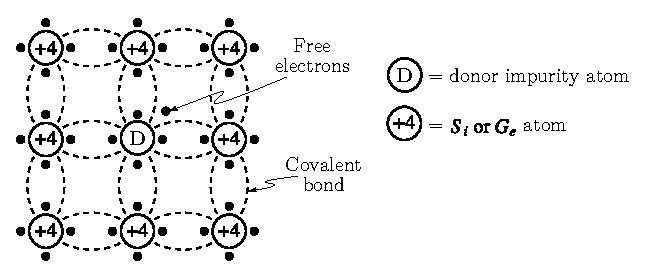
\includegraphics{chap1/fig1.11.eps}
\caption{Crystal lattice of Ge or Si atom displaced by an adom of a pentavalent impurity}\label{fig1.11}
\end{figure}

When donor impurities are added to semiconductor, allowable energy levels are introduced a very small distance below the conduction band as shown in Fig.~\ref{fig1.12}. The distance of the new discrete allowable energy level is approximately 0.01 eV below the conduction band for Ge and 0.05 eV for Si.
\begin{figure}[H]
\centering
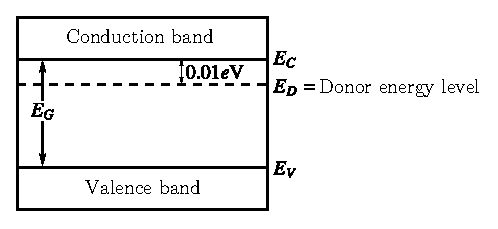
\includegraphics{chap1/fig1.12.eps}
\caption{Energy band diagram of n-type semiconductor (for Ge)}\label{fig1.12}
\end{figure}

A $p$-{\em type} material is produced by doping a semiconductor with impurity atoms that are trivalent (i.e., atom with 3 valence electrons). When this type of impurity atom is added to the intrinsic semiconductor, the three valence electrons form covalent bonds with neighbouring atoms of Ge or Si. One of the bonds, however is not complete as shown in Fig.~\ref{fig1.13}, since four valence electrons would be required and only three are available. This missing valance electron is called a {\em hole}.
\begin{figure}[H]
\centering
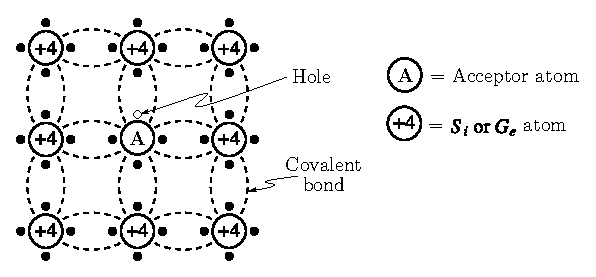
\includegraphics[scale=.93]{chap1/fig1.13.eps}
\caption{Crystal lattice of Si or Ge displaced by an atom of a trivalent impurity}\label{fig1.13}
\end{figure}

The trivalent impurity atoms used are called {\em acceptors} because the holes they produce can readily accept electron. Examples for acceptor impurity atoms are aluminium, boron, gallium and indium.

When an acceptor impurities are added to semiconductors they produce an allowable discrete energy level which is just above the valence band as shown in Fig.~\ref{fig1.14}.
\begin{figure}[H]
\centering
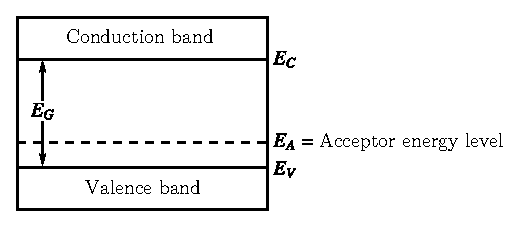
\includegraphics[scale=.93]{chap1/fig1.14.eps}
\caption{Energy band diagram of p-type semiconductor}\label{fig1.14}
\end{figure}

Although electrons are more than holes in n-type material, there are still a certain number of holes present due to temperature. The extent to which electrons dominate depends on the level of doping. The more heavily the material is doped with donor atoms, the greater the degree to which the number of electrons exceeds the number of holes. In n-type material electrons are the {\em majority} carriers and holes are the {\em minority} carriers. Similarly, the level of doping with acceptor impurity atoms controls the number of holes in p-type material. In p-type material, holes are the majority carriers and electrons are the minority carriers.

If a semiconductor material is doped with donor impurities not only does the number of electrons increases, but the number of holes decreases below that which would be available in the intrinsic semiconductor. The reason for the decrease in the number of holes is that the larger number of electrons present increase the rate of recombination of electrons with holes. Similarly, if a semiconductor material is doped with acceptor impurities not only does the holes increases but the number of electrons decreases below that which would be available in the intrinsic semiconductor.

However, the product of electron density `n' and hole density `p' would remain same and it is equal to the square of the intrinsic concentration.
\begin{equation}
\text{i.e.,}\quad \rmn\rmp=\rmn^{2}_{\rmi}\label{eq1.2}
\end{equation}
\begin{tabbing}
where ~ \= n = electron density (m$^{-3}$)\\[3pt]
        \> p = hole density (m$^{-3}$)\\[3pt]
        \> $\rmn_{\rmi}$ = intrinsic concentration (m$^{-3}$) 
\end{tabbing}
\noindent
Eqn.~\eqref{eq1.2} is known as {\em `law of mass action'}.

\section{Diffusion}\label{sec1.4}

In addition to a conduction current or drift current, there is another type of current due to the transport of charges in a semiconductor. This mechanism is called {\em diffusion} and the resulted current is called {\em diffusion current}. The diffusion is a flow of charge carriers from a region of high density to a region of low density due to the non-uniform distribution of it. The current density due to this diffusion is proportional to the carrier density gradient. The constant of proportionality called {\em diffusion constant} or {\em diffusion coefficient} $\rmD$ which has a unit of $\rmm^{2}/\sec$. 

\section{Qualitative theory of a PN junction}\label{sec1.5}

Consider a sample of single semi-conductor crystal which is doped to $\rmp$-type on one side and $\rmn$-type on the other. The area where the $\rmp$ and $\rmn$-type regions meet is called a $PN$ {\em junction} and the resulting device is a {\em diode}. Fig.~\ref{fig1.15} shows a simplified two dimensional view of such a PN junction diode at the instant they are formed.
\begin{figure}[H]
\centering
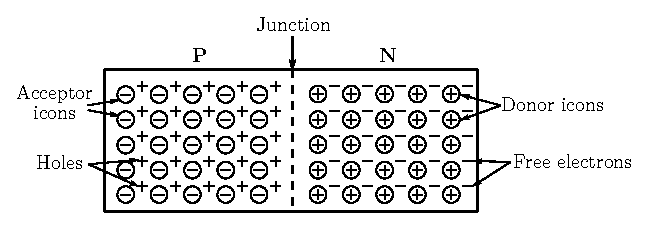
\includegraphics{chap1/fig1.15.eps}
\caption{A PN junction diode at the instant they are formed}\label{fig1.15}
\end{figure}

An acceptor ions and its associated holes are shown in the $\rmp$-region. The $\rmp$-region is initially neutral because the charge associated with each acceptor ion and that with each hole is equal in magnitude, opposite in sign and they are equal in numbers. Similarly, donor ions and its associated free electrons are shown in the $\rmn$-region. The $\rmn$-region is also initially neutral because the charge associated with each donor ion and that with each free electron is equal in magnitude, opposite in sign and they are also equal in numbers. Both acceptor and donor ions are not mobile whereas holes and free electrons are mobile.

Initially, at the instant the PN junction is formed, the density of holes in the $\rmp$-region and the density of free-electrons in the $\rmn$-region is large. Because of this density gradient across the junction, holes from the $\rmp$-side diffuse into the $\rmn$-side, where they combine with free-electrons. Similarly, free-electrons from the $\rmn$-side diffuse into the $\rmp$-side, where they combine with holes. This diffusion of holes and free-electrons is an electric current, known as {\em recombination current}. The recombination process decays exponentially with both time and distance from the junction. Thus, most of the recombination occurs very soon after the junction is formed and in the region very near to the junction. Thus the electrons have been removed and holes are added to the $\rmn$-side and the $\rmp$-side has lost holes and acquired electrons. This exchange of charge carrier occurs mainly in a small region on each side
of the junction which becomes depleted of charge carriers (i.e., holes and free electrons), leaving only uncovered negative acceptor ions on the $\rmp$-side and uncovered positive donor ions on the $\rmp$-side as shown in Fig.~\ref{fig1.16}. Therefore, this region is called {\em depletion region} or {\em space-charge region} or {\em transition region}.
\begin{figure}[H]
\centering
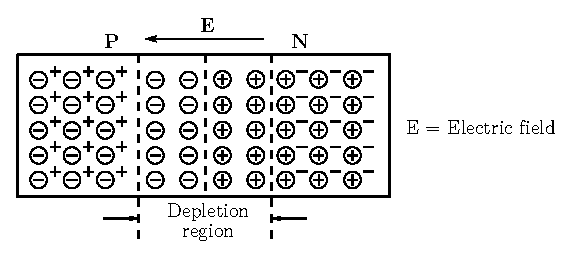
\includegraphics{chap1/fig1.16.eps}
\caption{The electric field due to the presence of uncovered ions in the depletion region near a PN junction.}\label{fig1.16}
\end{figure}

The physical width of the depletion region depends on the doping level. If very heavy doping is used, the depletion region is physically thin because a diffusing charge need not travel far across the junction before recombining.

\eject

The uncovered ions within the depletion region produce an electric field $\rmE$ as shown in Fig.~\ref{fig1.16}. This electric field represents a potential difference between the two regions and is called {\em barrier potential} or {\em space charge potential}. The barrier potential discourages further diffusion of charges across the junction. For example, an electron trying to diffuse from $\rmn$-side to $\rmp$-side is repelled by the negative acceptor ions on the $\rmp$-side. Similarly, a hole trying to diffuse from $\rmp$-side to $\rmn$-side is repelled by the positive donor ions on the $\rmn$-side. Therefore, the diffusion process does not continue indefinitely but continues till the electric field has grown up sufficiently to create enough barrier potential, which stops further diffusion. The value of the barrier potential $\rmV_{0}$ depends on the doping levels in the $\rmp$ and $\rmn$-region, the type of materials and the temperature. It is given by 
\begin{equation}
\rmV_{0}=\frac{\widetilde{\rmk}\rmT}{\rmq}\ln \left(\frac{\rmN_{\rmA}\rmN_{\rmD}}{\rmn^{2}_{i}}\right)\label{eq1.3}
\end{equation}
\begin{tabbing}
where\quad \= $\widetilde{\rmk}$ = Boltzmann constant = $1.381\times 10^{-23}$ J/$^{0}$K.\\[3pt]
      \> $\rmT$ = temperature in $^{0}\rmK$.\\[3pt]
      \> $\rmq$ = electron charge = $1.6\times 10^{-19}$ C.\\[3pt]
      \> $\rmN_{\rmA}$ = acceptor atom density in the $\rmp$-region (atoms/m$^{3}$).\\[3pt]
      \> $\rmN_{\rmD}$ = donor atom density in the $\rmn$-region (atoms/m$^{3}$).\\[3pt]
      \> $\rmn_{\rmi}$ = intrinsic concentration (carriers/m$^{3}$).
\end{tabbing}

\section{The PN junction as a diode}\label{sec1.6}

The important electrical characteristics of a PN junction is that it constitutes a diode which permits the easy flow of current in one direction but opposes the flow in the reverse direction.

\smallskip
\itheading{Forward bias~:} The word bias refers to a dc voltage that is applied across the junction by some externally connected source.

Suppose that an external voltage $\rmV$ is applied across a PN junction diode as shown in Fig.~\ref{fig1.17}(a). The $\rmp$-side is connected to the positive terminal of the battery and the $\rmn$-side to the negative terminal of the battery. In this case, the PN junction is said to be a {\em forward biased}. The external forward bias voltage creates an electric field across the junction whose direction opposes the internal electric field established by the depletion region. In other words, the barrier is reduced, so diffusion is enhanced. Therefore, current flows with relatively ease through the junction. The direction of conventional current is from $\rmp$ to $\rmn$ side as shown in the Fig.~\ref{fig1.17}(a) and (b).
\begin{figure}[H]
\centering
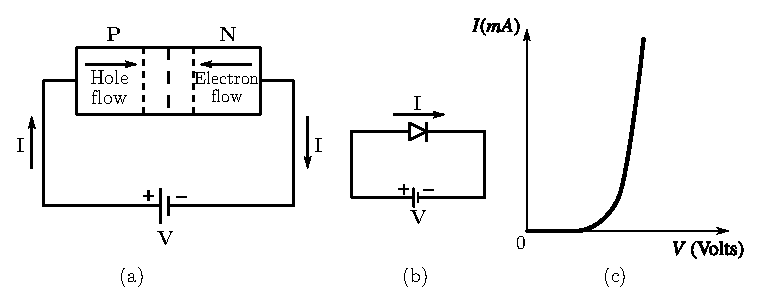
\includegraphics{chap1/fig1.17.eps}
\caption{(a) A forward biased PN junction diode. (b) A forward biased PN junction diode where diode is replaced by its symbol. (c) Forward biased VI characteristic of PN junction diode.}\label{fig1.17}
\end{figure}

When the PN junction is forward biased, the free electrons and the holes move towards the junction in the $\rmn$ and $\rmp$-region respectively. Thus, the current in each region is due to majority carriers. Since there is a reduction in the electric field at the forward biased junction, there is a corresponding reduction in the quantity of acceptor and donor ions to maintain the electric field. Therefore, the depletion region narrows under forward biased condition. As the forward biasing voltage $\rmV$ is increased to the extent that barrier potential has completely overcome, the majority charge carriers cross the junction easily, resulting in large current. Thus, under forward biased condition the current through the PN junction diode is due to majority carriers. The relationship between the voltage $\rmV$ and the current I through the junction is given by
\begin{equation}
\rmI=\rmI_{o}(\rme^{\rmV/\eta \rmV_{\rmT}}-1)\label{eq1.4}
\end{equation}

\noindent
\begin{tabbing}
where\quad \= $\rmI$ = current through the diode (A)\\[3pt]
           \> $\rmV$ = voltage across the junction (positive for forward bias) (V)\\[3pt]
           \> $\rmI_{o}$ = reverse saturation current\\[3pt]
           \> $\eta\simeq 1$ for Ge.\\[3pt]
           \> ~~ $\simeq 2$ for Si.\\[3pt]
           \> $\rmV_{\rmT}=\dfrac{\widetilde{\rmk}\rmT}{\rmq}$ = volt equivalent of temperature or thermal voltage.
\end{tabbing}

When the junction is forward biased (i.e., $\rmV$ is positive), the unity in Eqn.~\ref{eq1.4} may be neglected compared to the exponential term. It indicates that under forward biased condition, the current $\rmI$ increases exponentially with voltage $\rmV$ as shown in Fig.~\ref{fig1.17}(c).

\smallskip
\itheading{Reverse bias~:}
\begin{figure}[H]
\centering
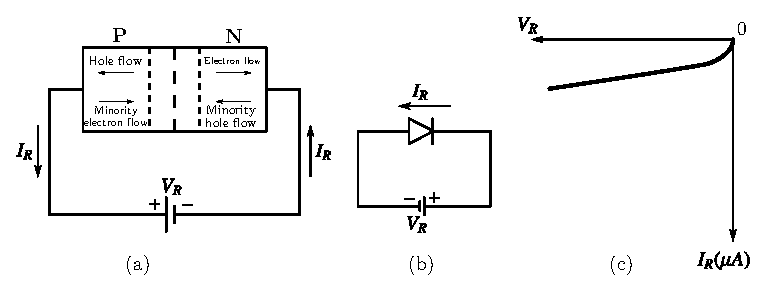
\includegraphics{chap1/fig1.18.eps}
\caption{(a) A reverse biased PN junction.\\ (b) A reverse biased PN junction diode where diode is replaced by its symbol.\\ (c) Reverse biased V-I characteristics of PN junction diode.}\label{fig1.18}
\end{figure}

Suppose that an external voltage is applied across a PN junction as shown in Fig.~\ref{fig1.18}(a). The $\rmp$-side is connected to the negative terminal of the battery and the $\rmn$-side to the positive terminal of the battery. In this case, the PN junction is said to be {\em reverse biased}. The external reverse bias voltage $\rmV_{\rmR}$ creates an electric field across the junction whose direction supports the internal electric field established by the depletion region. In other words, the barrier potential is increased and majority carrier find it more difficult to diffuse across the junction. In fact the majority carriers are pulled away from the junction and the junction provides very large resistance to the current flow.

But in addition to majority carriers, we also have minority carriers generated due to temperature on each side. The direction of electric field supports the movement of these minority carriers across the junction, but the current due to these minority carriers is very low. (in terms of microamps in Ge and nanoamps in Si).

When the junction is reverse biased (i.e., $\rmV$ is negative), the exponential term in Eqn.~\ref{eq1.4} may be neglected. Therefore, the reverse current $\rmI=\rmI_{\rmR}=-\rmI_{o}$, which is constant at a given temperature. But in practical, as the reverse bias voltage $\rmV_{\rmR}$ is increased in magnitude, the total current $\rmI_{\rmR}$ also increases slightly as shown in Fig.~\ref{fig1.18}(c). This is due to the impurities on the surface of the semiconductor, which behaves as an effective resistance, obeying Ohm's law. This component of current is known as {\em surface leakage current}.

Thus, the total reverse current $\rmI_{\rmR}$ is given by
\begin{equation}
\rmI_{\rmR}=\rmI_{\rmo}+\rmI_{\rmS}\label{eq1.5}
\end{equation}

\noindent
\begin{tabular}{@{}r@{\;\,}c@{\;\,}p{9cm}}
where~ $\rmI_{\rmo}$ & = & reverse saturation current due to minority charge carriers (temperature dependent).\\[3pt]
      $\rmI_{\rmS}$ & = & surface leakage current (voltage dependent). 
\end{tabular}

\smallskip
\itheading{Breakdown~:} If the reverse bias across a PN junction is increased beyond certain level known as {\em breakdown voltage}, the reverse current rises abruptly as shown in Fig.~\ref{fig1.19}.
\begin{figure}[H]
\centering
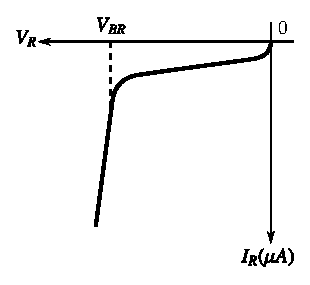
\includegraphics{chap1/fig1.19.eps}
\caption{Reverse biased characteristics of a PN junction diode including breakdown region}\label{fig1.19}
\end{figure}

The abrupt rise in reverse current may destruct the diode unless the current is limited to a safe value using external series resistor. There are two basic reasons which can cause the junction breakdown.
\begin{itemize}
\item[(i)] Zener breakdown

\item[(ii)] Avalanche breakdown
\end{itemize}

{\em Zener breakdown} is caused by strong electric field in the depletion region. A strong electric field can provide enough energy to break covalent bonds. As the external reverse bias increases, the electric field strength also increases, breaking more and more covalent bonds, thereby rising the current abruptly.

Another breakdown process is {\em avalanche}. This phenomenon generally occurs in wider depletion region, where the electric field strength is not strong enough to produce zener breakdown. Instead, free electrons (minory carriers) accelerated by the electron-hole pairs are created. This freed electrons are accelerated by the field, resulting in more collision, creating more free electrons. The process quickly avalanches to produce the abrupt rise in current.

The reverse voltage at which breakdown occurs can be controlled in the manufacturing process by varying the doping level.

\section{Volt - Ampere Characteristic}\label{sec1.7}

The relationship between voltage $\rmV$ across a PN junction diode and the current $\rmI$ through it is given by,
\begin{equation}
\rmI=\rmI_{\rmo}(\rme^{\rmV/\eta \rmV_{\rmT}}-1)\label{eq1.6}
\end{equation}

\noindent
\begin{tabular}{@{}r@{\;\,}c@{\;\,}p{10.5cm}}
where~ $\rmI$ & = & current through the PN junction diode\\[3pt]
      $\rmI_{\rmo}$ & = & reverse saturation current\\[3pt]
      $\rmV$ & = & voltage across the PN junction (positive for forward bias and negative for reverse bias)\\[3pt]
      $\eta$ & $\simeq$ & 1 for Ge\\[3pt]
             & $\simeq$ & 2 for Si\\[3pt]
      $\rmV_{\rmT}$ & = & $\dfrac{\widetilde{\rmk}\rmT}{\rmq}=$ volt equivalent of temperature or thermal voltage\\[3pt]
   $\widetilde{\rmk}$ & = & Boltzmann constant = $1.381\times 10^{-23}$ J/$^{0}$K\\[3pt]
   $\rmq$ & = & electron charge = $1.6\times 10^{-19}$ C
\end{tabular}

\medskip
The plot of V-I characteristics given in Eqn.~\eqref{eq1.6} is shown in Fig.~\ref{fig1.20}.
\begin{figure}[H]
\centering
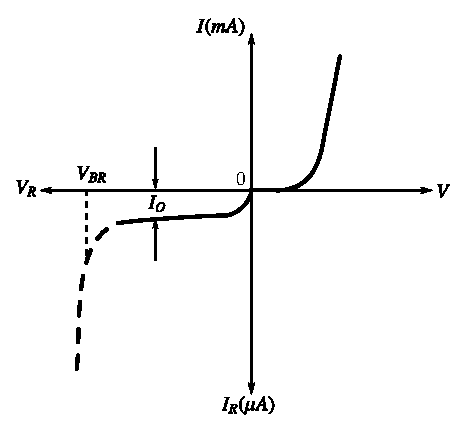
\includegraphics{chap1/fig1.20.eps}
\caption{V-I Characteristics of a PN junction diode}\label{fig1.20}
\end{figure}

When the diode is forward biased i.e., $\rmV$ is positive and several times $\rmV_{\rmT}$, the unity in the paranthesis in Eqn.~\eqref{eq1.6} may be neglected. Therefore, except for a small range in the neighbourhood of the origin, the current increases exponentially with voltage.

When the diode is reverse biased i.e., $\rmV$ is negative and several times greater than $\rmV_{\rmT}$ in magnitude, the exponential term in Eqn.~\eqref{eq1.6} may be neglected. Then $\rmI = -\rmI_{\rmo}$. The current $\rmI_{\rmo}$ is constant dependent on the temperature and is known as {\em reverse saturation current}.

\eqref{eq1.6} is called the {\em ideal diode equation}. In real diodes, the reverse current exceeds slightly the magnitude of $\rmI_{0}$. One reason for this is the existence of surface leakage current. Surface leakage current flows along the surface of the diode and obey's Ohm's law.

The Eqn.~\eqref{eq1.6} is not valid when the reverse bias across the PN junction is allowed to approach a certain value called the {\em reverse breakdown voltage} $\rmV_{\rmB\rmR}$. When the reverse bias voltage approaches $\rmV_{\rmB\rmR}$, a substantial reverse current flows. Furthermore, a very small increase in the reverse bias voltage in the vicinity of $\rmV_{\rmB\rmR}$ results in a very large increase in reverse current. The magnitude of the reverse current that flows when the reverse voltage $\rmV_{\rmR}$ approaches $\rmV_{\rmB\rmR}$ results in a very large increase in reverse current.

\begin{center}
\rule{4cm}{1pt}\\
{\bf\Large Problems}\\[-3pt]
\rule{4cm}{1pt}
\end{center}

\begin{problem}\label{prob1.1}
A germanium PN junction has a reverse saturation current of $1.9\times 10^{-10}$\,A. Assuming that $\eta=1$, find the current in the junction when the forward biasing voltage is 0.3 V and the temperature is $27^{\circ}$C.
\end{problem}

\begin{solution}
Given~: $\rmV=0.3\rmV$, \ $\eta=1$, \ $\rmI_{0}=1.9\times 10^{-10}\rmA$

$T=27^{\circ}\rmC= (273+27^{0})\rmK=300^{0}\rmK$.
\begin{align*}
\text{Thermal voltage~~} \rmV_{\rmT} &= \frac{\widetilde{\rmk}\rmT}{\rmq}=\frac{1.381\times 10^{-23}\times 300}{1.6\times 10^{-19}}\\[3pt]
&= \simeq 26~\text{mV}
\end{align*}

We have,
\begin{align*}
\rmI &= \rmI_{\rmo}(\rme^{\rmV/\eta\rmV_{\rmT}}-1)\\[3pt]
     &= 1.9\times 10^{-10}\left(e^{\frac{0.3}{1\times 26\times 10^{-3}}}-1\right)\\[3pt]
     &= 0.0195\text{~mA.}
\end{align*}
$\therefore$~ The current in the PN junction diode $\rmI = 0.0195$ mA.
\end{solution}

\eject

\begin{problem}\label{prob1.2}
The forward current in a PN junction is 1.5 mA at $27^{\circ}$C. If reverse saturation current is $2.4\times 10^{-14}$A and $\eta=1$, what is the forward biasing voltage across the junction ?
\end{problem}

\begin{solution}
Given~: \ $\rmI=1.5\text{~mA}$, $\rmT=27^{\circ}\rmC=(273+27)^{0}\rmK=300^{0}\rmK$.
$$
\eta = 1,\quad \rmI_{\rmo}=2.4\times 10^{-14}\rmA, \ \rmV_{\rmT}=\dfrac{\widetilde{k}\rmT}{\rmq}=26\text{~mV}.
$$

We have, $\rmI=\rmI_{\rmo}(\rme^{\rmV/\eta \rmV_{\rmT}}-1)$
\begin{align*}
\therefore\quad \rme^{\rmV/\eta \rmV_{\rmT}} &= \frac{\rmI}{\rmI_{\rmo}}+1=\frac{1.5\times 10^{-3}}{2.4\times 10^{-14}}+1\\[5pt]
&= 6.25\times 10^{10}
\end{align*}

Taking log on both the sides, we get
\begin{align*}
\frac{\rmV}{\eta\rmV_{\rmT}} &= 24.858\\[5pt]
\rmV &= 1\times 26\times 10^{-3}\times 24.858\\[5pt]
\rmV &= 0.646\rmV.
\end{align*}
$\therefore$~ The forward biasing voltage $\rmV=0.646\rmV$.
\end{solution}

\begin{problem}\label{prop1.3}
A junction diode is connected across an external voltage source so that the negative terminal of the source is connected to the anode of the diode. If the external source is 5V and the reverse saturation current is 0.06 pA, what is the diode current ? (neglect surface leakage current).
\end{problem}

\begin{solution}
Since the negative terminal of the source is connected to the anode of the diode, it is reverse biased.

We have, \ $\rmI=\rmI_{\rmo}(\rme^{\rmV/\eta \rmV_{\rmT}-1})$

In this equation, exponential term may be neglected when $\rmV$ is negative. 
$$
\therefore\quad \rmI=-\rmI_{\rmo}=-0.06\text{~pA.}
$$

$\therefore$~ The diode current $\rmI=\rmI_{\rmo}=-0.06$ pA. The negative sign indicates that the conventional current is from cathode to anode.
\end{solution}

\eject

\begin{problem}\label{prob1.4}
A germanium diode carries a current of 10 mA when a forward bias of 0.2V is applied across it at $27^{\circ}$C.
\begin{itemize}
\item[(a)] Find the reverse saturation current.

\item[(b)] Calculate the bias voltage needed for diode currents of 1mA and 100mA.
\end{itemize}
\end{problem}

\begin{solution}
\begin{itemize}
\item[(a)] Given~: $I=10\text{~mA}$, \ $\rmV=0.2\rmV$, \ $\eta=1$ \ for \ Ge

$\rmT=27^{\circ}\rmC=(273+27)^{0}\rmK=300^{0}K$

We have
\begin{align*}
\rmI &= \rmI_{\rmo}(\rme^{\rmV/\eta \rmV_{\rmT}-1})\simeq \rmI_{\rmo}e^{\rmV/\eta \rmV_{\rmT}}\\[3pt]
\therefore\quad \rmV_{\rmT} &= \frac{\widetilde{\rmk}\rmT}{\rmq}=\frac{1.381\times 10^{-23}\times 300}{1.6\times 10^{-19}}=26\text{~mV}.\\[3pt]
\rmI_{\rmo} &= \frac{\rmI}{\rme^{\rmV/\eta \rmV_{\rmT}}}=\frac{10\times 10^{-3}}{\rme^{\frac{0.2}{1\times 26\times 10^{-3}}}}\\[3pt]
\rmI_{\rmo} &= 4.56\mu \rmA.
\end{align*}
$\therefore$~ the reverse saturation current~ $\rmI_{\rmo}=4.42\mu\rmA$.

\item[(b)] To calculate the voltage needed for diode current of 1 mA.
\begin{align*}
\rmI &= \rmI_{\rmo}\rme^{\rmV/\eta \rmV_{\rmT}}\\[3pt]
\rme^{\rmV/\eta \rmV_{\rmT}} &= \frac{\rmI}{\rmI_{\rmo}}\\[3pt]
\frac{\rmV}{\eta \rmV_{\rmT}} &= \ln \left(\frac{\rmI}{\rmI_{\rmo}}\right)\\[3pt]
\rmV &= \eta \rmV_{\rmT}\ln \left(\frac{\rmI}{\rmI_{\rmo}}\right)\\[3pt]
\text{For}\quad \rmI &= 1\text{~mA},\\[3pt]
\rmV &= 1\times 26\times 10^{-3}\times \ln (4.56\times 18)\\[3pt]
&= 0.140\rmV
\end{align*}
Similarly for $\rmI=100\text{~mA}$ \ \ $\rmV=0.259\rmV$
\end{itemize}
\end{solution}

\section{Diode Resistances}\label{sec2.8}

As the operating point of a diode moves from one region to another the resistance of the diode will also change due to the non-linear shape of its VI-characteristics.

\smallskip
\heading{D-C or Static Resistance}

The application of a dc voltage to a circuit containing a semiconductor diode will result in an operating point on the VI-characteristic curve that will not change with time. The resistance of the diode at this operating point is called dc or static resistance. It can be found simply by finding the corresponding levels of $\rmV_{\rmD}$ and $\rmI_{\rmD}$ as shown in the Fig.~\ref{fig1.21} below.
\begin{figure}[H]
\centering
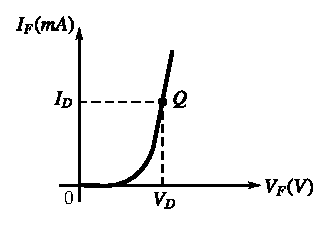
\includegraphics{chap1/fig1.21.eps}
\caption{}\label{fig1.21}
\end{figure}

$Q$ = Operating point.

DC or Static resistance is $\rmR_{\rmD}=\dfrac{\rmV_{\rmD}}{\rmI_{\rmD}}$ Lower the value of the current through the diode, the higher the value of dc or static resistance.

\smallskip
\heading{AC or Dynamic Resistance}
\smallskip

If a sinusoidal voltage is applied across a diode, the instantaneous operating point will move up and down on the characteristics. This indicates that there exists a particular change in current when there is a change in current with time. The resistance offered by the diode to this variation of current is called ac or dynamic resistance.

This resistance value can be obtained from the characteristics as shown below.

AC or dynamic resistance is given by,
$$
\rmr_{\rmd}=\dfrac{\Delta \rmV_{\rmD}}{\Delta \rmI_{\rmD}}
$$

In general, the lower the $Q$-point of operation (i.e., smaller current or smaller voltage) the higher the ac resistance.
\begin{figure}[H]
\centering
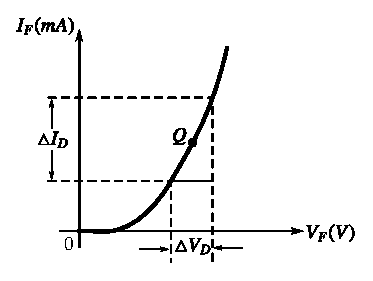
\includegraphics[scale=.95]{chap1/fig1.22.eps}
\caption{}\label{fig1.22}
\end{figure}

\vskip -.5cm
\heading{Average AC Resistance}
\smallskip

If the ac input voltage applied across the diode is sufficiently large to produce a wide swing of current through it, the resistance associated for this region is called average ac resistance. The average ac resistance can be determined by a straight line drawn between the two intersections established by the maximum and minimum values of input voltage as shown below.
\begin{figure}[H]
\centering
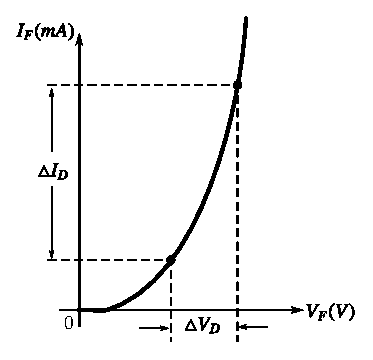
\includegraphics[scale=.95]{chap1/fig1.23.eps}
\caption{}\label{fig1.23}
\end{figure}
$$
\text{Average ac resistance~~ } \rmr_{\rma\rmV}=\dfrac{\Delta \rmV_{\rmD}}{\Delta \rmI_{\rmD}}\Big/\text{pt to pt.}
$$


\section{Diode Equivalent Circuits}\label{sec1.9}

\heading{Equivalent Circuit~:} Equivalent circuit (or model) is a proper combination of electrical elements like voltage source, current source, resistors etc. to best represent the actual terminal characteristics of a device or system.

\vfill\eject

The equivalent circuit for a diode can be obtained by approximating the VI characteristics by straight-line segments. Basically, there are 3 equivalent circuits or approximations. They are,
\begin{itemize}
\item[(i)] Ideal approximation.\qquad (ii)~ Simplified approximation.

\item[(iii)] Piecewise-linear approximation.
\end{itemize}

\heading{(i)~ Ideal approximation.}

In this approximation, both $\rmV_{\rmr}$ (cut-in voltage) and $\rmR_{\rmf}$ (diode forward resistance) are ignored. The VI characteristics and the equivalent circuit (model) are shown below.
\begin{figure}[H]
\centering
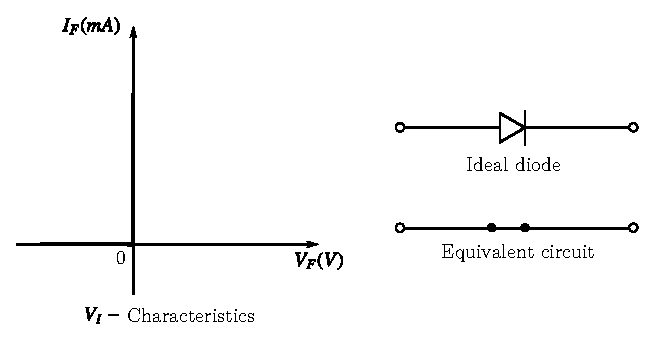
\includegraphics[scale=.91]{chap1/fig1.24.eps}
\caption{}\label{fig1.24}
\end{figure}

\heading{(ii)~ Simplified Approximation~:} In this approximation, only $\rmV_{\rmr}$ (cut-in voltage) is considered and $\rmR_{\rmf}$ (diode forward resistance) is ignored. The VI-characteristics and the equivalent circuit are shown below.
\begin{figure}[H]
\centering
\includegraphics[scale=.91]{chap1/fig1.25.eps}
\caption{}\label{fig1.25}
\end{figure}

\heading{(iii)~ Piecewise-linear Approximation~:} In this approximation, both $\rmV_{\rmr}$ and $\rmR_{\rmf}$ are considered. The VI-characteristics and the equivalent circuit are shown below.
\begin{figure}[H]
\centering
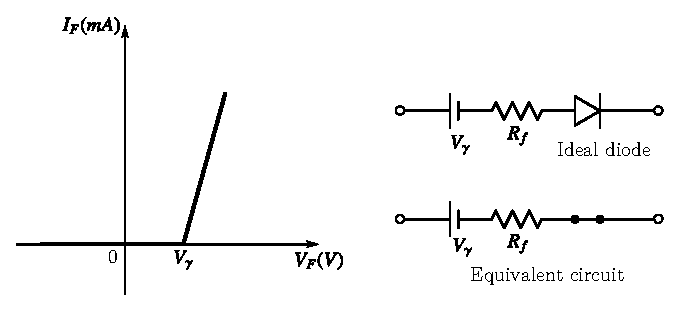
\includegraphics{chap1/fig1.26.eps}
\caption{}\label{fig1.26}
\end{figure}

\heading{Transition and Diffusion Capacitance}

There exist 2 types of capacitance effects when using PN junction diode at very high frequencies. 
\begin{itemize}
\item[(i)] Transition or depletion or space charge capacitance $(\rmC_{\rmT})$ 

(when the diode is reverse biased)

\item[(ii)] Diffusion or storage capacitance $(\rmC_{\rmD})$

(when the diode is forward biased)
\end{itemize}

We know that the capacitance of a parallel-plate capacitor is given by $\rmC=\dfrac{\rmA\epsilon}{d}$.

\begin{tabbing}
where\quad \=$\epsilon$ is the premittivity of the dialectric between the plates.\\[3pt]
\>$\rmA$ is the area of plates.\\[3pt]
\>$\rmd$ is the distance between the plates.
\end{tabbing}

\noindent
when the diode is reverse biased, there exist a depletion region (free of carriers) that behaves like a dielectric between the layers of opposite charge. This results in transition capacitance and is denoted by $\rmC_{\rmT}$.

Since the depletion region width $\rmd$ will increase with increased reverse bias, the resulting transition capacitance will decrease as shown below.

When the diode is forward biased, there exist a capacitance effect called diffusion or storage capacitance and denoted by $\rmC_{\rmD}$. This capacitance effect is directly dependent on the rate at which charge is injected into the regions just outside the depletion region. The value of diffusion capacitance increases with increase in forward bias. The graph of capacitances $\rmV_{\rms}$ the bias voltage is shown below. The capacitance effects described above are represented by a capacitor in parallel with the ideal diode.
\begin{figure}[H]
\centering
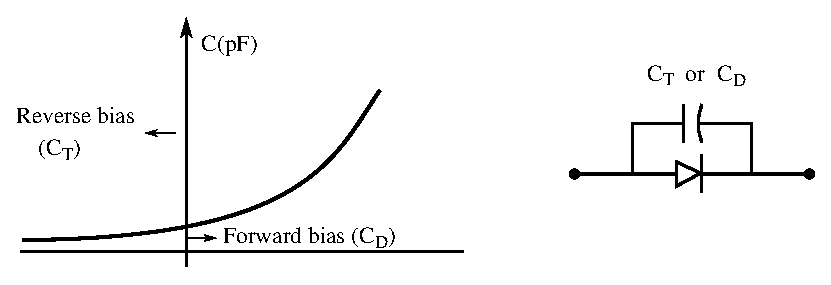
\includegraphics{chap1/addfig1.eps}
\end{figure}

\heading{Reverse Recovery Time : \boldmath$(\rmt_{\rmr\rmr})$}
\begin{figure}[H]
\centering
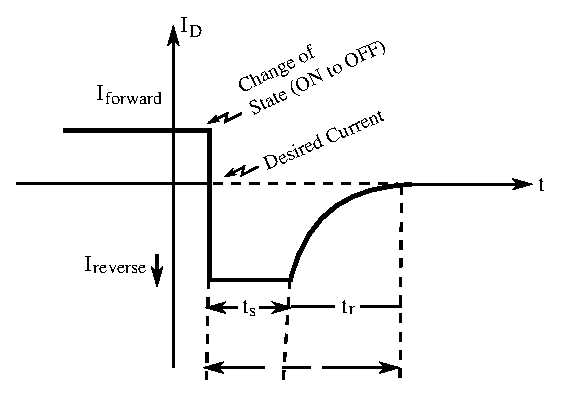
\includegraphics{chap1/addfig2.eps}
\end{figure}
In the forward biased condition the large number of free electrons from $\rmN$-side flow towards $\rmp$ side and large number of holes from $\rmp$-side flow towards $\rmN$-side. Once free electrons reaches $\rmP$-side and holes $\rmN$-side their status will become minority charge carriers. If the diode is reverse biased suddenly the current through it will not become zero instantaneously became of accumulated minority charge carriers on $\rmP$ and $\rmN$. These minority charge carriers will cross the junction because reverse bias supports it and it results in a large reverse current. This large reverse current will stay for a measurable amount of time known as storage time $(\rmt_{\rms})$. Once the flow of minority charge carriers are over, the current will reduce to the non-conduction state and the time taken for this proce is called reverse recovery time $(\rmt_{\rmr})$.

Thus the reverse recovery time is the sum of these two intervals. i.e., $\rmt_{\rmr\rmr}=\rmt_{\rms}+\rmt_{\rmr}$.


Most commercially avails switching diodes $\rmt_{\rmr\rmr}$ is in the range of $1\mu\rms$.


\smallskip
\heading{DC Load Line Analysis}

Consider the network shown below.
\begin{figure}[H]
\centering
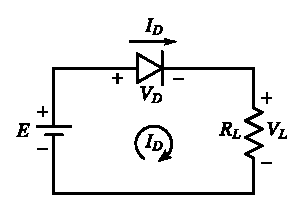
\includegraphics{chap1/fig1.27.eps}
\caption{}\label{fig1.27}
\end{figure}

In the network, the diode is forward biased and the voltage drop across the diode is $\rmV_{\rmD}$ and the current through the diode is $\rmI_{\rmD}$.

Applying KVL to the circuit, we get
\begin{align}
& \rmE -\rmV_{\rmD}-\rmV_{\rmL}=0\notag\\[3pt]
\text{or}\quad &\rmE=\rmV_{\rmD}+\rmV_{\rmL}\notag\\[3pt]
\text{i.e.,}\quad &\rmE=\rmV_{\rmD}+\rmI_{\rmD}\cdot \rmR_{\rmL}\label{eq1.7}
\end{align}

The two variables in \eqref{eq1.7} are $\rmV_{\rmD}$ and $\rmI_{\rmD}$.

When $\rmV_{\rmD}=0$ in Eqn.~\eqref{eq1.7}; 
$$
\rmI_{\rmD}=\left. \dfrac{\rmE}{\rmR_{\rmL}}\right|_{\rmV_{\rmD=0}}\quad [\rmV_{\rmD}=0\text{~~ means vertical axis}]
$$
and when $\rmI_{\rmD}=0$ in Eqn.~\eqref{eq1.7};
$$
\rmV_{\rmD}=\rmE\big|_{\rmI_{\rmD}=0}\quad [\rmI_{\rmD}=0\text{~~ means horizontal axis}]
$$

A straight line drawn between these 2 points is known as load-line. The point of intersection of this load-line with the characteristics of the diode is called quiescent point (Q point) or operating point.
\begin{figure}[H]
\centering
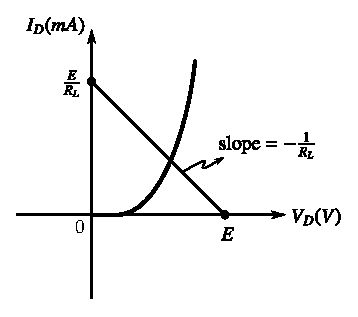
\includegraphics{chap1/fig1.28.eps}
\caption{}\label{fig1.28}
\end{figure}

\section{Rectifiers}\label{sec1.10}

Every electronic circuit requires a dc power source. This dc power can be obtained by dc power supply or batteries. But usually batteries are used for power supply in portable electronic equipments. However, it is economical and convenient to obtain this dc power from dc power supply which is usually consists rectifier, filter and regulator to convert ac power into dc power.

A rectifier is an electronic circuit used for converting ac voltage or current into dc voltage or current. Basically, rectifiers are classified into two categories depending upon the period of conduction.
\begin{itemize}
\item[(a)] Half-wave Rectifier\qquad (b)~ Full-wave Rectifier
\end{itemize}

\subsection{Half-wave Rectifier}\label{sec1.10.1}

Fig.~\ref{fig1.29} shows the circuit diagram of a half wave rectifier. The ac voltage to be rectified is applied across the primary of the transformer and that across the secondary is available for rectification.
\begin{figure}[H]
\centering
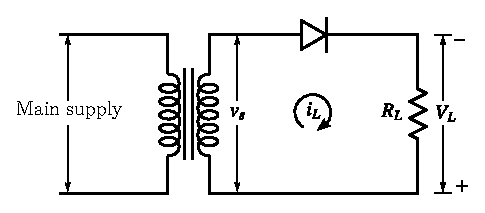
\includegraphics{chap1/fig1.29.eps}
\caption{Half-wave rectifier}\label{fig1.29}
\end{figure}

Let the voltage across the secondary of the transformer available for rectification be,
\begin{equation}
\upsilon_{\rms}=\rmV_{\rmm}\sin \omega\, \rmt \label{eq1.8}
\end{equation}

During positive cycle of $\upsilon_{\rms}$ diode conducts and during negative cycle of $\upsilon_{\rms}$ diode does not conduct.
\begin{figure}[H]
\centering
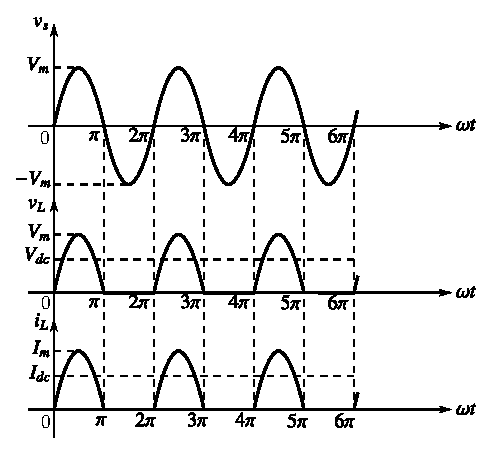
\includegraphics[scale=1.15]{chap1/fig1.30.eps}
\caption{Half-wave rectified output waveform}\label{fig1.30}
\end{figure}

Assuming that cut-in voltage of the diode is zero and $\rmR_{\rmf}$ is the forward resistance of the diode, the voltage across the load,
\begin{align*}
\upsilon_{\rmL} &= \rmv_{\rms}\text{~~ during positive cycle of } \upsilon_{\rms}.\\[3pt]
         &= 0\text{~ during negative cycle of~ } \upsilon_{\rms}.
\end{align*}
\begin{equation}
\text{Peak current~~} \rmI_{\rm}=\frac{\rmV_{\rmm}}{\rmR_{\rmf}+\rmR_{\rmL}}\label{eq1.9}
\end{equation}

Fig.~\ref{fig1.30} shows waveforms of $\upsilon_{\rms}$, load voltage $\upsilon_{\rmL}$ and load current $\rmi_{\rmL}$.

\eject

The average or dc value of the load current is
\begin{align}
\rmI_{\rmd\rmc} &= \frac{1}{2\pi}\int\limits^{2\pi}_{0}\rmi_{\rmL} \rmd \omega\, \rmt\notag\\[4pt]
\rmI_{\rmd\rmc} &= \frac{1}{2\pi}\int\limits^{\pi}_{0}\rmI_{\rmm}\sin \omega\, t\quad \rmd\omega\, \rmt\quad [\because~ \text{diode conducts only between } 0<\omega\, \rmt<\pi]\notag\\[4pt]
&= \frac{-\rmI_{\rmm}}{2\pi}[\cos\omega\, \rmt]^{\pi}_{0}\notag\\[5pt]
\rmI_{\rmd\rmc} &= \frac{\rmI_{\rmm}}{\pi}\label{eq1.10}
\end{align}

DC voltage across the load 
\begin{align}
\rmV_{\rmd\rmc} &=\rmI_{\rmd\rmc}\cdot \rmR_{\rmL}\notag\\[5pt]
&= \frac{\rmI_{\rmm}}{\pi}\cdot \rmR_{\rmL}\notag\\[5pt]
&= \frac{\rmV_{\rmm}\rmR_{\rmL}}{\pi(\rmR_{i}+\rmR_{\rmL})}\notag\\[5pt]
&= \frac{\rmV_{\rmm}}{\pi\left(1+\frac{\rmR_{\rmf}}{\rmR_{\rmL}}\right)}\notag\\[5pt]
\therefore\quad \rmV_{\text{dc}} &\simeq \frac{\rmV_{\rmm}}{\pi}\quad [\because \ \rmR_{\rmf}\ll \rmR_{\rmL}]\label{eq1.11}
\end{align}

The rms value of the load current $i_{\rmL}$ is
\begin{align}
\rmI_{\text{rms}} &= \sqrt{\frac{1}{2\pi}\int\limits^{2\pi}_{0}i_{\rmL^{2}}\rmd \omega\, \rmt}\notag\\[3pt]
&= \sqrt{\frac{1}{2\pi}\int\limits^{\pi}_{0}\rmI^{2}_{\rmm}\sin^{2}\omega\,\rmt. d\omega\,\rmt}\notag\\[3pt]
\rmI_{\text{rms}} &= \frac{I_{m}}{2}\label{eq1.12}
\end{align}

\eject

The rms voltage across the load
\begin{align}
\rmV_{\text{rms}} &= \rmI_{\text{rms}}\cdot \rmR_{\rmL}\notag\\[4pt]
&= \frac{\rmI_{\rmm}}{2}\cdot \rmR_{\rmL}\notag\\[4pt]
&= \frac{\rmV_{\rmm}\rmR_{\rmL}}{2(\rmR_{\rmf}+\rmR_{\rmL})}\notag\\[4pt]
&= \frac{\rmV_{\rmm}}{2(1+\rmR_{\rmf}/\rmR_{\rmL})}\notag\\[4pt]
\rmV_{\text{rms}} &\simeq \frac{\rmV_{\rmm}}{2}\quad [\because \ \rmR_{\rmf}\ll \rmR_{\rmL}]\label{eq1.13}
\end{align}

\heading{Efficiency \boldmath$\eta$~:}
It is defined as the ratio of dc power delivered to the load to the ac power supplied from the secondary of the transformer.

\vskip .1cm
DC power delivered to the load $\rmP_{\text{dc}}=\rmI_{\text{dc}}^{2}\rmR_{\rmL}=\dfrac{\rmI^{2}_{\rmm}\rmR_{\rmL}}{\pi^{2}}$

\vskip .15cm
AC power supplied from the secondary of the transformer
\begin{align}
\rmP_{\text{ac}} &= \rmI^{2}_{\text{rms}}(\rmR_{\rmf}+\rmR_{\rmL})\notag\\[5pt]
&= \frac{I^{2}_{\rmm}}{4}(\rmR_{\rmf}+\rmR_{\rmL})\notag\\[5pt]
\therefore\quad \text{Efficiency~~ } \eta &= \frac{\rmP_{\text{dc}}}{\rmP_{\text{ac}}}\notag\\[5pt]
&= \frac{\rmI^{2}_{\rmm}\rmR_{\rmL}/\pi^{2}}{\rmI^{2}_{\rmm}(\rmR_{\rmf}+\rmR_{\rmL})/4}\notag\\[5pt]
&= \frac{4}{\pi^{2}}\cdot f\frac{\rmR_{\rmL}}{\rmR_{\rmf}+\rmR_{\rmL}}\notag\\[5pt]
\eta &= \frac{0.406}{1+\frac{\rmR_{\rmf}}{\rmR_{\rmL}}}\label{eq1.14}
\end{align}

Thus, the rectifier efficiency increases as the ratio $\rmR_{\rmf}/\rmR_{\rmL}$ reduces. Theoritically, the maximum value of efficiency of a half-wave rectifier is 40.6\%\ corresponding to the value of $\rmR_{\rmf}/\rmR_{\rmL}$ equal to zero.

\eject

\heading{Ripple factor \boldmath$r$~:} It is defined as the ratio of the rms value of the ac component of voltage or current to the dc value of voltage or current.
\begin{align*}
\rmr &= \frac{\rmI_{\rmr, \text{rms}}}{\rmI_{\text{dc}}}\\[3pt]
&= \frac{\sqrt{\rmI^{2}_{\text{rms}}-\rmI^{2}_{\text{dc}}}}{\rmI_{\text{dc}}}\quad [\because \ \rmI^{2}_{\text{rms}}=\rmI^{2}_{\text{dc}}+\rmI^{2}_{\rmr,\text{rms}}]\\[3pt]
&= \sqrt{\left(\frac{\rmI_{\text{rms}}}{\rmI_{\text{dc}}}\right)^{2}-1}= \sqrt{\left(\frac{\rmI_{\rmm}/2}{\rmI_{\rmm}/\pi}\right)^{2}-1}\\[3pt]
\rmr &= 1.21
\end{align*}

It indicates that, in a half-wave rectifier the ac component across the load $\rmR_{\rmL}$ is 1.21 times that of dc component, (ideal case).

\smallskip
\heading{Peak-inverse voltage (PIV)~:} The peak inverse voltage rating of a diode determines its maximum permissible reverse bias without breakdown. The diode in half-wave rectifier must be capable of with standing a peak reverse voltage of $\rmV_{\rmm}$ volts.
$$
\text{i.e.,}\quad \text{PIV} \geq \rmV_{\rmm}
$$

\smallskip
\heading{Regulation~:} It is a measure of how well the rectifier is able to maintain a constant voltage between no-load and full-load conditions.
$$
\text{i.e.,~~ Percentage regulation } = \frac{\rmV_{\text{NL}}-\rmV_{\text{FL}}}{\rmV_{\text{FL}}}\times 100\%
$$

For half-wave rectifier, the percentage regulation is
\begin{align*}
&= \frac{\frac{\rmV_{\rmm}}{\pi}-\rmI_{\text{dc}}\rmR_{\rmL}}{\rmI_{\text{dc}}\rmR_{\rmL}}\times 100\%\\[3pt]
&= \frac{\frac{\rmV_{\rmm}}{\pi}-\frac{\rmI_{\rmm}}{\pi}\cdot \rmR_{\rmL}}{\frac{\rmI_{\rmm}}{\pi}\cdot \rmR_{\rmL}}\times 100\%\\[3pt]
&= \frac{\frac{\rmV_{\rmm}}{\pi}-\frac{\rmV_{\rmm}\rmR_{\rmL}}{\pi(\rmR_{\rmf}+\rmR_{\rmL})}}{\frac{\rmV_{\rmm}\rmR_{\rmL}}{\pi(\rmR_{\rmf}+\rmR_{\rmL})}}\times 100\%
\end{align*}
Percentage regulation $=\dfrac{\rmR_{\rmf}}{\rmR_{\rmL}}\times 100\%$.

\begin{center}
\rule{4cm}{1pt}\\
{\bf\Large Problems}\\[-3pt]
\rule{4cm}{1pt}
\end{center}

\begin{problem}\label{prob1.5}
A sinusoidal voltage of peak value 40 V and frequency 50 Hz is applied to a half-wave rectifier. No filter is used. The load resistor is 800 $\Omega$. Neglecting the cut-in voltage and using idealized characteristics for the diode with $\rmR_{\rmf}=8\Omega$ and $\rmR_{\rmf}=\infty$, calculate,
\begin{itemize}
\item[(a)] peak, dc and rms values of load current.

\item[(b)] dc output power.

\item[(c)] ac input power.

\item[(d)] rectifier efficiency.
\end{itemize}
\end{problem}

\begin{solution}
Given $\rmV_{\rmm}=40\rmV$, \ $\rmf=50\text{~Hz}$, \ $\rmR_{\rmL}=800\Omega$, \ $\rmR_{\rmf}=8\Omega$, \ $\rmR_{\rmf}=\infty$.
\begin{itemize}
\item[(a)] Peak current \ $\rmI_{\rmm}=\dfrac{\rmV_{\rmm}}{\rmR_{\rmf}+\rmR_{\rmL}}=\dfrac{40}{(8+800)}=49.5\text{~mA}$

\vskip .1cm
dc current \ $\rmI_{\text{dc}}=\dfrac{\rmI_{\rmm}}{\pi}=\dfrac{49.5\times 10^{-3}}{\pi}=15.75\text{~mA}$

\vskip .1cm
rms current \ $\rmI_{\text{rms}}=\dfrac{\rmI_{\rmm}}{2}=\dfrac{49.5\times 10^{-3}}{2}=24.75\text{~mA}$

\smallskip
\item[(b)] dc output power
\begin{align*}
\rmP_{\text{dc}} &= \rmI^{2}_{\text{dc}}\cdot \rmR_{\rmL}\\[3pt]
              &= (15.75\times 10^{-3})^{2}\times 800\\[3pt]
              &= 198.45\text{~mW}
\end{align*}

\item[(c)] ac input power
\begin{align*}
\rmP_{\text{ac}} &= \rmI^{2}_{\text{rms}}(\rmR_{\rmf}+\rmR_{\rmL})\\[3pt]
&= (24.75\times 10^{-3})^{2}\times (8+800)\\[3pt]
&= 494.95\text{~mW}.
\end{align*}

\item[(d)] Rectifier efficiency
\begin{align*}
\eta &= \frac{\rmP_{\text{dc}}}{\rmP_{\text{ac}}}\\[3pt]
&= \frac{198.45\times 10^{-3}}{494.95\times 10^{-3}}\\[3pt]
&\simeq 40.09\%
\end{align*}
\end{itemize}
\end{solution}

\begin{problem}\label{prob1.6}
A half-wave rectifier uses a transformer with turns ratio $2:1$. The load resistance is $500\Omega$. If the primary voltage is $240\rmV$, 50 Hz, calculate,
\begin{itemize}
\item[(a)] the peak inverse voltage

\item[(b)] the dc output voltage
\end{itemize}
Neglect cut-in voltage and forward resistance of the diode.
\end{problem}

\begin{solution}
Given~: $\rmN_{1}:\rmN_{2}=2:1$, \ $\rmR_{\rmL}=500\Omega$
\begin{align*}
\text{Primary voltage~ } &= 240 \rmV_{\text{rms}}\\[3pt]
\therefore\quad \text{Secondary voltage~ } &= \frac{1}{2}\times 240 = 120\rmV_{\text{rms}}\\[3pt]
\therefore\quad \text{Peak voltage} \rmV_{\rmm} &= \sqrt{2}\times 120=169.7\rmV 
\end{align*}
\begin{itemize}
\item[(a)] In half-wave rectifier \ PIV = $\rmV_{\rmm}=169.7\rmV$

\item[(b)] Peak current $\rmI_{\rmm}=\dfrac{\rmV_{\rmm}}{\rmR_{\rmL}}=\dfrac{169.7}{500}=339.4$ mA

dc output current $\rmI_{\text{dc}}=\dfrac{\rmI_{\rmm}}{\pi}=\dfrac{339.4\times 10^{-3}}{\pi}=108.04$~ mA
\begin{align*}
\therefore~ \text{dc output voltage } \rmV_{\text{dc}} &= \rmI_{\text{dc}}\cdot \rmR_{\rmL}\\[3pt]
&= (108.04\times 10^{-3})\times 500\\[3pt]
&= 54.02\rmV
\end{align*}
\end{itemize}
\end{solution}

\begin{problem}\label{prob1.7}
What peak-to-peak sinusoidal voltage must be connected to a half-wave rectifier if the rectified waveform is to have a dc value of 6 V. ? Assume that the forward drop across the diode is 0.7 V.
\end{problem}

\begin{solution}
Given \ $\rmV_{\text{dc}}=6 \rmV$.

\vskip .1cm
Considering forward drop of 0.7 V across the diode.
\begin{align*}
\rmV_{\text{dc}} &= \frac{\rmV_{\rmm}}{\pi}-0.7\\[5pt]
\therefore\quad \rmV_{\rmm} &= \pi (\rmV_{\text{dc}}+0.7)\\[5pt]
&= \pi(6+0.7)\\[5pt]
\rmV_{\rmm} &= 21.048\rmV
\end{align*}
\vskip -.7cm
\begin{align*}
\therefore\quad \text{Peak-to-peak voltage required~ } = 2\rmV_{\rmm} &= 2\times 21.048\\[5pt]
                       &= 42.097\rmV
\end{align*}
\end{solution}

\begin{problem}\label{prob1.8}
The output voltage and current waveform of a half-wave rectifier is shown in Fig.~\ref{fig1.31}. Determine the value load resistor, output dc current, input ac current and the efficiency. Assume the diode is ideal.
\begin{figure}[H]
\centering
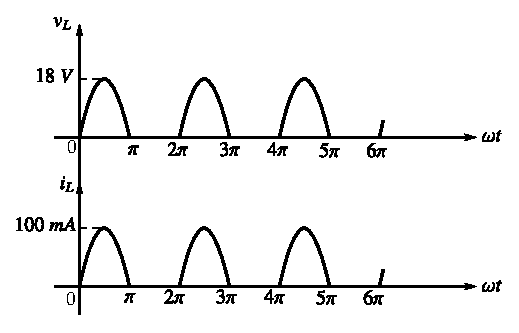
\includegraphics{chap1/fig1.31.eps}
\caption{}\label{fig1.31}
\end{figure}
\end{problem}

\begin{solution}
From the output waveform we have $\rmV_{\rmm}=18\rmV$ and $\rmI_{\rmm}=100\text{~mA}$. Since the diode is ideal, we have
\begin{align*}
\rmI_{\rmm} &= \frac{\rmV_{\rmm}}{\rmR_{\rmL}}\\[5pt]
\therefore\quad \text{load resistor~ } \rmR_{\rmL} &= \frac{\rmV_{\rmm}}{\rmI_{\rmm}}=\frac{18}{100\times 10^{-3}}=180\Omega\\[4pt]
\text{output dc current~ } \rmI_{\text{dc}} &= \frac{\rmI_{\rmm}}{\pi}=\dfrac{100\times 10^{-3}}{\pi}=31.83\text{~mA}\\[5pt]
\text{input ac current~ } \rmI_{\text{rms}} &= \frac{\rmI_{\rmm}}{2}=\frac{100\times 10^{-3}}{2}=50\text{~mA}\\[5pt]
\text{Efficiency~ } \eta &= \frac{\rmP_{\text{dc}}}{\rmP_{\text{ac}}}\times 100=\frac{\rmI^{2}_{\text{dc}}\rmR_{\rmL}}{\rmI_{\text{rms}}^{2}(\rmR_{\rmf}+\rmR_{\rmL})}\times 100\\[4pt]
&=\frac{\rmI^{2}_{\text{dc}}}{\rmI^{2}_{\text{rms}}}\times 100 \ [\because \ \rmR_{\rmf}=0]\\[5pt]
&= \frac{(31.83\times 10^{-3})^{2}}{(50\times 10^{-3})^{2}}\times 100\%\\[5pt]
&= 40.5\%
\end{align*}
\end{solution}

\subsection{Full-wave rectifier}\label{sec1.10.2}

Fig.~\ref{fig1.32} shows the circuit diagram of centre-tapped transformer full-wave rectifier. The ac voltage to be rectified is applied across the primary of the transformer and that across the secondary is available for rectification.
\begin{figure}[H]
\centering
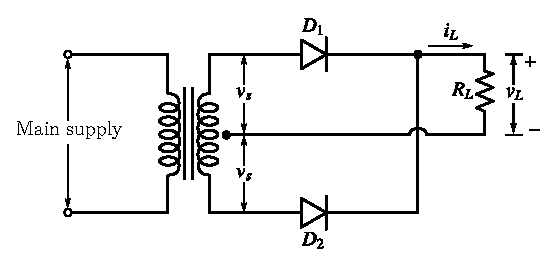
\includegraphics{chap1/fig1.32.eps}
\caption{Centre-tapped transformer full-wave rectifier}\label{fig1.32}
\end{figure}

Let the voltage across the half of the secondary winding of the transformer available for rectification be
$$
\upsilon_{\rms}=\rmV_{\rmm}\sin \omega\, \rmt
$$

\eject

During positive cycle of $\upsilon_{\rms}$, diode $\rmD_{1}$ conducts and during negative cycle diode $\rmD_{2}$ conducts. But under both the situations the current flowing through the load $\rmR_{\rmL}$ is unidirectional.
\begin{figure}[H]
\centering
\includegraphics[scale=1.1]{chap1/fig1.33.eps}
\caption{Full-wave rectified input and output waveform}\label{fig1.33}
\end{figure}

Consider that the cut-in voltage of the diodes are zero and $\rmR_{\rmf}$ is the forward resistance of each diode, then we have,
\begin{equation}
\text{Peak current~ } \rmI_{\rmm}=\dfrac{\rmV_{\rmm}}{\rmR_{\rmf}+\rmR_{\rmL}}\label{eq1.15}
\end{equation}

\vskip .1cm
Fig.~\ref{fig1.33} shows the waveform of $\upsilon_{\rms}$, load voltage $\upsilon_{\rmL}$ and load current $\rmi_{\rmL}$.

\vskip .1cm
The average or dc value of load current $\rmi_{\rmL}$ is
\begin{align}
\rmI_{\text{dc}} &= \frac{1}{\pi}\int\limits^{\pi}_{0}\rmi_{\rmL}d\omega\, \rmt\notag\\[5pt]
&= \frac{1}{\pi}\int\limits^{\pi}_{0}\rmI_{\rmm}\sin \omega\,\rmt \ d\omega\, \rmt\notag\\[5pt]
\rmI_{\text{dc}} &= \frac{2\rmI_{\rmm}}{\pi}\label{eq1.16}
\end{align}

\eject

\noindent
$\therefore$~ DC voltage across the load
\begin{align}
\rmV_{\text{dc}} &= \rmI_{\text{dc}}\cdot \rmR_{\rmL}\notag\\[3pt]
&= \frac{2\rmI_{\rmm}}{\pi}\cdot \rmR_{\rmL}\notag\\[3pt]
&= \frac{2}{\pi}\cdot \frac{\rmV_{\rmm}}{(\rmR_{\rmf}+\rmR_{\rmL})}\cdot \rmR_{\rmL}\notag\\[3pt]
&= \frac{2}{\pi}\cdot \frac{\rmV_{\rmm}}{\left(1+\frac{\rmR_{\rmf}}{\rmR_{\rmL}}\right)}\notag\\[3pt]
\therefore\quad \rmV_{\text{dc}} &\simeq \frac{2\rmV_{\rmm}}{\pi}\quad [\because \ \rmR_{\rmf}ll \rmR_{\rmf}]\label{eq1.17}
\end{align}
The rms value of the load current $i_{\rmL}$ is
\begin{align}
\rmI_{\text{rms}} &= \sqrt{\frac{1}{\pi}\int\limits^{\pi}_{0}i_{\rmL^{2}}\rmd \omega\, \rmt}\notag\\[3pt]
&= \sqrt{\frac{1}{\pi}\int\limits^{\pi}_{0}\rmI^{2}_{\rmm}\sin^{2}\omega\,\rmt \ \rmd \omega\,\rmt}\notag\\[3pt]
&= \sqrt{\frac{\rmI^{2}_{\rmm}}{2\pi}\int\limits^{\pi}_{0}(1-\cos 2\omega\, \rmt)d\omega\, \rmt}\notag\\[3pt]
\therefore\quad \rmI_{\text{rms}} &= \frac{\rmI_{\rmm}}{\sqrt{2}}\label{eq1.18}
\end{align}

The rms voltage across the load,
\begin{align}
\rmV_{\text{rms}} &= \rmI_{\text{rms}}\cdot \rmR_{\rmL}\notag\\[3pt]
&= \frac{\rmI_{\rmm}}{\sqrt{2}}\cdot \rmR_{\rmL}\notag\\[3pt]
&= \frac{1}{\sqrt{2}}\cdot \frac{\rmV_{\rmm}}{\rmR_{\rmf}+\rmR_{\rmL}}\cdot \rmR_{\rmL}\notag\\[3pt]
&= \frac{\rmV_{\rmm}}{\sqrt{2}}\cdot \frac{1}{\left(1+\frac{\rmR_{\rmf}}{\rmR_{\rmL}}\right)}\notag\\[3pt]
\therefore\quad \rmV_{\text{rms}} &\simeq \frac{\rmV_{\rmm}}{\sqrt{2}}\quad [\because \ \rmR_{\rmf}\ll \rmR_{\rmL}]\label{eq1.19}
\end{align}

\heading{Efficiency \boldmath$\eta$~:} It is defined as the ratio of dc power delivered to the load to the ac power supplied from the secondary of the transformer.

DC power delivered to the load $\rmP_{\text{dc}}=\rmI^{2}_{\text{dc}}\cdot \rmR_{\rmL}=\left(\dfrac{2\rmI_{\rmm}}{\pi}\right)^{2}\cdot \rmR_{\rmL}$

AC power supplied from the secondary of the transformer
\begin{align}
\rmP_{\text{ac}} &= \rmI^{2}_{\text{rms}}(\rmR_{\rmf}+\rmR_{\rmL})\notag\\[3pt]
              &= \left(\dfrac{\rmI_{\rmm}}{\sqrt{2}}\right)^{2}(\rmR_{\rmf}+\rmR_{\rmL})\notag\\[3pt]
\therefore~ \text{Efficiency ~ }\eta &= \frac{\rmP_{\text{dc}}}{\rmP_{\text{ac}}}\notag\\[3pt]
&= \frac{\left(\frac{2\rmI_{\rmm}}{\pi}\right)^{2}\cdot \rmR_{\rmL}}{(\rmI_{\rmm}/\sqrt{2})^{2}(\rmR_{\rmf}+\rmR_{\rmL})}\notag\\[3pt]
\eta &= \frac{0.81}{1+\frac{\rmR_{\rmf}}{\rmR_{\rmL}}}\label{eq1.20}
\end{align}

Theoritically, the maximum value of efficiency of a full-wave rectifier is 81\%\ corresponding to the value of $\rmR_{\rmf}/\rmR_{\rmL}$ equal to zero.

\smallskip
\heading{Ripple factor \boldmath$r$~:} It is defined as the ratio of the rms value of the ac component of voltage or current to the dc value of voltage or current.
\begin{align}
\therefore\quad \rmr &= \frac{\rmI_{\rmr, \text{rms}}}{\rmI_{\text{dc}}}\notag\\[3pt]
&= \frac{\sqrt{\rmI_{\text{rms}}^{2}-\rmI^{2}_{\text{dc}}}}{\rmI_{\text{dc}}}\qquad [\because \ \rmI^{2}_{\text{rms}}=\rmI^{2}_{\text{dc}}+\rmI^{2}_{\text{r, rms}}]\notag\\[3pt]
&= \sqrt{\left(\frac{\rmI_{\text{rms}}}{\rmI_{\text{dc}}}\right)^{2}-1}\notag\\[3pt]
&= \sqrt{\frac{(\rmI_{\rmm}/\sqrt{2})^{2}}{(2\rmI_{\rmm}/\pi)^{2}}-1}\notag\\[3pt]
\rmr &\simeq 0.483\label{eq1.21}
\end{align}

It indicates that in centre-tapped transformer full-wave rectifier the ac component across the load $\rmR_{\rmL}$ is 0.483 times that of dc component. (ideal case).

\smallskip
\heading{Peak inverse voltage~:} Each diode in centre-tapped full-wave rectifier must be capable of withstanding a peak reverse voltage of $2\rmV_{\rmm}$ volts.
$$
\text{i.e.,}\qquad \text{PIV~ }\geq 2\rmV_{\rmm}\text{~~ volts.}
$$
\begin{align}
\text{Voltage regulation~ } &= \frac{\rmV_{\text{NL}}-\rmV_{\text{FL}}}{\rmV_{\text{FL}}}\times 100\%\notag\\[3pt]
&= \frac{\frac{2\rmV_{\rmm}}{\pi}-\rmI_{\text{dc}}\rmR_{\rmL}}{\rmI_{\text{dc}}\rmR_{\rmL}}\times 100\%\notag\\[3pt]
&= \frac{\frac{2\rmV_{\rmm}}{\pi}-\frac{2\rmI_{\rmm}}{\pi}\cdot \rmR_{\rmL}}{\frac{2\rmI_{\rmm}}{\pi}\cdot \rmR_{\rmL}}\times 100\%\notag\\[3pt]
\text{Voltage regulation~ } &= \frac{\rmR_{\rmf}}{\rmR_{\rmL}}\times 100\%\label{eq2.22}
\end{align}

\medskip

\begin{center}
\rule{4cm}{1pt}\\
{\bf\Large Problems}\\[-3pt]
\rule{4cm}{1pt}
\end{center}

\begin{problem}\label{prob1.9}
A full-wave p-n diode rectifier uses load resistor $\rmR_{\rmL}=1100\Omega$. No filter is used. Assume each diode have ideal characteristics with $\rmR_{\rmf}=10\Omega$ and $\rmR_{\rmr}=\infty$. The cut-in voltage is neglected. If sinusoidal voltage with amplitude 20 V is applied to each diode, calculate
\begin{itemize}
\item[(a)] peak, dc and rms values of load current

\item[(b)] dc output power

\item[(c)] ac input power

\item[(d)] percentage efficiency.
\end{itemize}
\end{problem}

\begin{solution}
Given \ $\rmV_{\rmm}=20\rmV$, \ $\rmR_{\rmL}=1100\Omega$, \ $\rmR_{\rmf}=10\Omega$, \ $\rmR_{\rmr}=\infty$.
\begin{itemize}
\item[(a)] Peak current $\rmI_{\rmm}=\dfrac{\rmV_{\rmm}}{\rmR_{\rmf}+\rmR_{\rmL}}=\dfrac{20}{10+1100}=18.01$~ mA.

\smallskip
\quad dc current $\rmI_{\text{dc}}=\dfrac{2\rmI_{\rmm}}{\pi}=\dfrac{2\times 18.01\times 10^{-3}}{\pi}=11.47$~mA

\smallskip
rms current $\rmI_{\text{rms}}=\dfrac{\rmI_{\rmm}}{\sqrt{2}}=\dfrac{18.01\times 10^{-3}}{\sqrt{2}}=12.73$ mA.

\smallskip
\item[(b)]
\begin{tabbing}
dc output power \ $\rmP_{\text{dc}}$ \== $\rmI^{2}_{\text{dc}}\rmR_{\rmL}$\\[4pt]
                                  \>= $(11.47\times 10^{-3})^{2}\times 1100$\\[4pt]
                                  \>= $144.7$~ mW
\end{tabbing}

\item[(c)]
\begin{tabbing}
ac input power \ $\rmP_{\text{ac}}$ \== $\rmI^{2}_{\text{rms}}(\rmR_{\rmf}+\rmR_{\rmL})$\\[4pt]
                                 \>= $(12.73\times 10^{-3})^{2}(10+1100)$\\[4pt]
                                 \>= $179.87$~ mW
\end{tabbing}

\item[(d)] 
\begin{tabbing}
Percentage efficiency \ $\eta$ \== $\dfrac{\rmP_{\text{dc}}}{\rmP_{\text{ac}}}\times 100\%$\\[4pt]
                               \>= $\dfrac{144.7\times 10^{-3}}{179.87\times 10^{-3}}\times 100\%$\\[4pt]
                               \>= $80.4\%$
\end{tabbing}
\end{itemize}
\end{solution}

\begin{problem}\label{prob1.10}
A full-wave rectifier supplies a load of 10 k$\Omega$. The ac voltage applied to the diode is 300-0-300 $\rmV_{\text{rms}}$. If the diode forward resistance is neglected, calculate,
\begin{itemize}
\item[(a)] dc output current\qquad (b)~ dc output voltage\qquad (c)~ ripple voltage.
\end{itemize}
\end{problem}

\begin{solution}
Given~:~ $\rmV_{\rmm}=\sqrt{2}\times 300=424.26\rmV$, \ $\rmR_{\rmL}=10$ k$\Omega$.
\begin{align*}
\therefore\quad \text{Peak current~ } \rmI_{\rmm} = \frac{\rmV_{\rmm}}{\rmR_{\rmf}+\rmR_{\rmL}} &= \frac{\rmV_{\rmm}}{\rmR_{\rmL}}\quad [\because \ \rmR_{\rmf}=0]\\[5pt]
&= \dfrac{424.26}{10\times 10^{3}}\\[5pt]
&= 42.43\text{~mA}
\end{align*}
\begin{itemize}
\item[(a)] 
\begin{tabbing}
dc output current \ $\rmI_{\text{dc}}$ \== $\dfrac{2\rmI_{\rmm}}{\pi}$\\[5pt]
                                    \>= $\dfrac{2\times 42.43\times 10^{-3}}{\pi}$\\[5pt]
                                    \>= 27 mA
\end{tabbing}

\item[(b)]
\begin{tabbing}
dc output voltage \ $\rmV_{\text{dc}}$ \== $\rmI_{\text{dc}}\rmR_{\rmL}$\\[5pt]
                                    \>= $(27\times 10^{-3})\times (10\times 10^{3})$\\[5pt]
                                    \>= 270 V.
\end{tabbing}

\eject

\item[(c)] 
\begin{tabbing}
ripple factor \ r \== $\sqrt{\left(\dfrac{\rmI_{\text{rms}}}{\rmI_{\text{dc}}}\right)^{2}-1}$\\[5pt]
                             \>= $\sqrt{\left(\dfrac{\rmI_{\rmm}/\sqrt{2}}{2\rmI_{\rmm}/\pi}\right)^{2}-1}$\\[5pt]
                             \>= 0.48
\end{tabbing}

\item[(d)] Also we have $\rmr = \dfrac{\rmI_{\rmr,\text{rms}}}{\rmI_{\text{dc}}}=0.48$
\begin{align*}
\text{output ripple current~ } \rmI_{\rmr, \text{rms}} &= 0.48\times \rmI_{\text{dc}}\\[3pt]
 &= 0.48\times 27\times 10^{-3}\\[3pt]
&= 12.96\text{~mA}\\[3pt]
\therefore\quad \text{ripple voltage~~~ } \rmV_{\rmr,\text{rms}} &= \rmI_{\rmr,\text{rms}}\rmR_{\rmL}\\[3pt]
&= (12.96\times 10^{-3})\times (10\times 10^{3})\\[3pt]
&= 129.6\rmV
\end{align*}
\end{itemize}
\end{solution}

\begin{problem}\label{prob1.11}
The primary voltage in the circuit shown in Fig.~\ref{fig1.34} is 120 $\rmV_{\text{rms}}$ and the transformer ratio is $\rmN_{1}:\rmN_{2}=4:1$. Find
\begin{itemize}
\item[(a)] the average value of the voltage across $\rmR_{\rmL}$.

\item[(b)] the average power dissipated by $\rmR_{\rmL}$.

\item[(c)] the minimum PIV rating required for each diode.
\end{itemize}
Assume that cut-in voltage of each diode $\rmV_{\gamma}=0.7\rmV$ and $\rmR_{\rmf}=0\Omega$.
\begin{figure}[H]
\centering
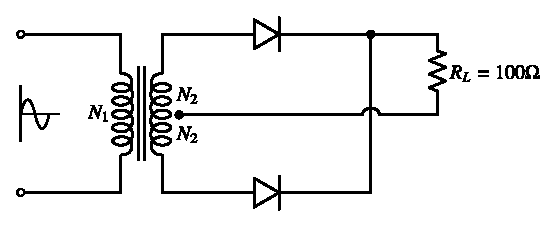
\includegraphics{chap1/fig1.34.eps}
\caption{}\label{fig1.34}
\end{figure}
\end{problem}

\begin{solution}
Given $\rmN_{1}:\rmN_{2}=4:1$, \ $\rmR_{\rmL}=100\Omega$.
\begin{align*}
\text{Maximum primary voltage~~ } \rmV_{\rmP} &= \sqrt{2}\times 120\\[4pt]
                                             &= 169.7\rmV\\[4pt]
\therefore\quad \text{Maximum secondary voltage~~ } \rmV_{\rmS} &= \frac{\rmN_{2}}{\rmN_{1}}\times \rmV_{\rmP}\\[4pt]
&= \frac{1}{4}\times 169.7\\[4pt]
&= 42.42\rmV
\end{align*}
If cut-in voltage of each diode is 0.7 V, the maximum voltage across the load.
\begin{align*}
\rmV_{\rmm} &= \rmV_{\rmS}-0.7\\[4pt]
          &= 42.42-0.7\\[4pt]
          &= 41.7\rmV
\end{align*}
\begin{itemize}
\item[(a)] 
\begin{tabbing}
Average or dc voltage across load $\rmR_{\rmL}:\rmV_{\text{dc}}$ \== $\dfrac{2\rmV_{\rmm}}{\pi}$\\[7pt]
                                                             \>= $\dfrac{2\times 41.7}{\pi}$\\[7pt]
                                                             \>= 26.56 V
\end{tabbing}

\item[(b)] 
\begin{tabbing}
Average power dissipated by $\rmR_{\rmL}$ \ $\rmP_{\text{dc}}$ \== $\dfrac{\rmV^{2}_{\text{dc}}}{\rmR_{\rmL}}$\\[7pt]
                                                           \>= $\dfrac{(26.56)^{2}}{100}$\\[7pt]
                                                           \>= 7.06 W
\end{tabbing}

\item[(c)] 
\begin{tabbing}
Minimum PIV rating required for each diode \== $2\times (42.42)$\\[3pt]
                                           \>= $84.84$ V
\end{tabbing}
\end{itemize}
\end{solution}

\begin{problem}\label{prob1.13}
The secondary winding of a centre-tapped transformer is rated at 15-0-15 V. Determine the dc output voltage, the dc load current and peak inverse voltage rating required for the diodes, if this transformer is used to excite a full-wave rectifier with a load resistance of $100\Omega$. Assume diodes are ideal.
\end{problem}

\eject

\begin{solution}
Given~:
\vskip -.4cm
\begin{align*}
\rmV_{\rmm} &=\sqrt{2}\times 15=21.2\rmV\\[3pt]
\rmR_{\rmL} &= 100\Omega.
\end{align*}
\begin{tabbing}
Diode is ideal\qquad~~ $\therefore$~ $\rmR_{\rmf}$ \ \== $0 \ \Omega$ \  and \ $\rmV_{\gamma}=0$ V\\[7pt]
Peak load current\qquad~ $\rmI_{\rmm}$ \ \>= $\dfrac{\rmV_{\rmm}}{\rmR_{\rmL}}$\quad $[\because \ \rmR_{\rmf}\cong 0]$\\[6pt]
                       \>= $\dfrac{21.21}{100}= 212.1$ mA\\[6pt]
$\therefore$~~ dc load current\quad~~~ $\rmI_{\text{dc}}$ \ \>= $\dfrac{2\rmI_{\rmm}}{\pi}$\\[6pt]
                       \>= $\dfrac{2(212.1\times 10^{-3})}{\pi}= 135.1$ mA\\[6pt]
$\therefore$~~ dc output voltage~~ $\rmV_{\text{dc}}$ \ \>= $\rmI_{\text{dc}}\cdot \rmR_{\rmL}$\\[6pt]
                       \>= $(135.1\times 10^{-3})\times 100= 13.5\rmV$
\end{tabbing}

\begin{tabbing}
The PIV rating of the diodes must be greater than $2\rmV_{\rmm}$ \== $2\times 21.21$\\[4pt]
                                                               \>= $42.42\rmV$
\end{tabbing}
\end{solution}

\subsection{Bridge rectifier}\label{sec1.10.3}

Fig.~\ref{fig1.35} shows the circuit diagram of a full-wave bridge rectifier. The ac voltage to be rectified is applied across the primary of the transformer and that across the secondary is available for rectification.

Let the voltage across the secondary of the transformer available for rectification be
$$
\upsilon_{\rms}=\rmV_{\rmm}\sin \omega\, \rmt
$$
\begin{figure}[H]
\centering
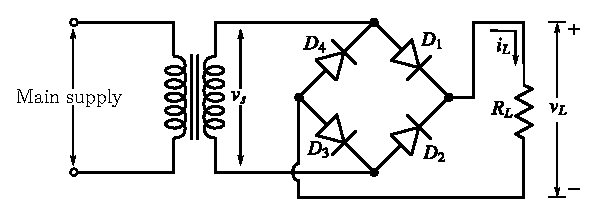
\includegraphics{chap1/fig1.35.eps}
\caption{Full-wave bridge rectifier}\label{fig1.35}
\end{figure}

During positive cycle of $\upsilon_{\rms}$, diode $\rmD_{1}$ and $\rmD_{3}$ conducts and during negative cycle $\rmD_{2}$ and $\rmD_{4}$ conducts. But under both the situations the current flowing through the load resistor $\rmR_{\rmL}$ is unidirectional.

Consider that cut-in voltage of all the diodes are zero and $\rmR_{\rmf}$ is the forward resistance of each diode. Then we have,
\begin{equation}
\text{Peak current}\quad \rmI_{\rmm}=\dfrac{\rmV_{\rmm}}{2\rmR_{\rmf}+\rmR_{\rmL}}\label{eq1.23}
\end{equation}

At a time two diodes conduct. Thus, $2\rmR_{\rmf}$ in the denominator of Eqn.~\eqref{eq1.23}.

Fig.~\ref{fig1.36} shows the waveform of $\upsilon_{\rms}$, load voltage $\upsilon_{\rmL}$ and load current $\rmi_{\rmL}$,
\begin{figure}[H]
\centering
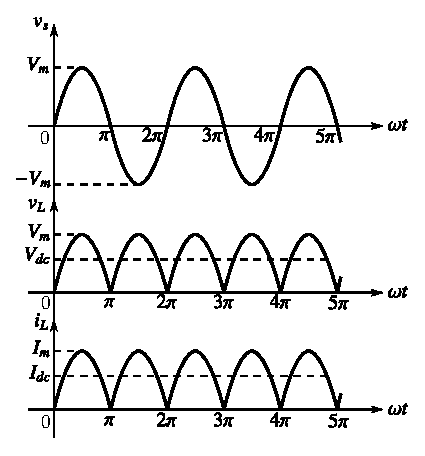
\includegraphics{chap1/fig1.36.eps}
\caption{Input and output waveforms of full-wave bridge rectifier}\label{fig1.36}
\end{figure}

The average or dc value of the load current $\rmi_{\rmL}$ is,
\begin{align}
\rmI_{\text{dc}} &= \frac{1}{\pi}\int\limits^{\pi}_{0}\rmi_{\rmL}\rmd\omega\,\rmt\notag\\[4pt]
\rmI_{\text{dc}} &= \frac{1}{\pi}\int\limits^{\pi}_{0}\rmI_{\rmm}\sin \omega\,\rmt \ \rmd\omega\,\rmt\notag\\[4pt]
\rmI_{\text{dc}} &= \frac{2\rmI_{\rmm}}{\pi}\label{eq1.24}
\end{align}

The dc voltage across the load is
\begin{align}
\rmV_{\text{dc}} &= \rmI_{\text{dc}}\cdot \rmR_{\rmL}\notag\\[5pt]
&= \frac{2\rmI_{\rmm}}{\pi}\cdot \rmR_{\rmL}\notag\\[5pt]
&= \frac{2}{\pi}\left[\frac{\rmV_{\rmm}}{2\rmR_{\rmf}+\rmR_{\rmL}}\right]\cdot \rmR_{\rmL}\notag\\[5pt]
&= \frac{2\rmV_{\rmm}}{\pi\left(1+\frac{2\rmR_{\rmf}}{\rmR_{\rmL}}\right)}\notag\\[5pt]
\therefore\quad \rmV_{\text{dc}} &\simeq \frac{2\rmV_{\rmm}}{\pi}\quad [\because \ \rmR_{\rmf}\ll \rmR_{\rmL}]\label{eq1.25}
\end{align}

The rms value of the load current $\rmi_{\rmL}$ is
\begin{align}
\rmI_{\text{rms}} &= \sqrt{\frac{1}{\pi}\int\limits^{\pi}_{0}\rmi_{\rmL}^{2} \rmd\omega\,\rmt}\notag\\[5pt]
&= \sqrt{\frac{1}{\pi}\int\limits^{\pi}_{0}\rmI^{2}_{m}\sin^{2}\omega\,\rmt \ \rmd\omega\,\rmt}\notag\\[5pt]
\rmI_{\text{rms}} &= \frac{\rmI_{\rmm}}{\sqrt{2}}\label{eq1.26}
\end{align}

The rms voltage across the load is
\begin{align}
\rmV_{\text{rms}} &= \rmI_{\text{rms}}\cdot \rmR_{\rmL}\notag\\[5pt]
&= \frac{\rmI_{\text{m}}}{\sqrt{2}}\cdot \rmR_{\rmL}\notag\\[5pt]
&= \frac{1}{\sqrt{2}}\left[\frac{\rmV_{\rmm}}{2\rmR_{\rmf}+\rmR_{\rmL}}\right]\cdot \rmR_{\rmL}\notag\\[5pt]
&= \frac{\rmV_{\rmm}}{\sqrt{2}\left(1+\frac{2\rmR_{\rmf}}{\rmR_{\rmL}}\right)}\notag\\[5pt]
\therefore\quad \rmV_{\text{rms}} &\simeq \frac{\rmV_{\rmm}}{\sqrt{2}}\quad [\because \ \rmR_{\rmf}\ll \rmR_{\rmL}]\label{eq1.27}
\end{align}
        
\heading{Efficiency \ \boldmath$\eta$~:} It is defined as the ratio of dc power delivered to the load to the ac power supplied from the secondary of the transformer.

\begin{tabbing}
DC power delivered to the load \ $\rmP_{\text{dc}}$ \== $\rmI^{2}_{\text{dc}}\cdot \rmR_{\rmL}$\\[4pt]
                                                 \>= $\left(\dfrac{2\rmI_{\rmm}}{\pi}\right)^{2}\cdot \rmR_{\rmL}$
\end{tabbing}

\begin{tabbing}
AC power supplied from the secondary of the transformer \ $\rmP_{\text{ac}}$ \== $\rmI^{2}_{\text{rms}}(2\rmR_{\rmf}+\rmR_{\rmL})$\\[4pt]
\>= $\left(\dfrac{\rmI_{\rmm}}{\sqrt{2}}\right)(2\rmR_{\rmf}+\rmR_{\rmL})$
\end{tabbing}
\begin{align}
\therefore\quad \text{Efficiency~~ } \eta &= \frac{\rmP_{\text{dc}}}{\rmP_{\text{ac}}}\notag\\[4pt]
&= \frac{(2\rmI_{\rmm}/\pi)^{2}\cdot \rmR_{\rmL}}{(\rmI_{\rmm}/\sqrt{2})^{2}(2\rmR_{\rmf}+\rmR_{\rmL})}\notag\\[4pt]
\eta &= \frac{0.81}{1+\frac{2\rmR_{\rmf}}{\rmR_{1}}}\label{eq}
\end{align}

Theoritically, the maximum value of efficiency of a full-wave bridge rectifier is 81\%\ corresponding to the value of $2\rmR_{\rmf}/\rmR_{\rmL}$ equal to zero.

\smallskip
\heading{Ripple factor \boldmath$\rmr$~:} It is defined as the ratio of the rms value of the ac component of voltage or current to the dc value of voltage or current.
\begin{align*}
\text{i.e.,}\qquad \rmr &= \frac{\rmI_{\rmr,\text{rms}}}{\rmI_{\text{dc}}}\\[4pt]
 &= \frac{\sqrt{\rmI^{2}_{\text{rms}}-\rmI^{2}_{\text{dc}}}}{\rmI_{\text{dc}}}\qquad [\because \ \rmI^{2}_{\text{rms}}=\rmI^{2}_{\text{dc}}+\rmI^{2}_{\rmr,\text{rms}}]\\[4pt]
&= \sqrt{\left(\frac{\rmI_{\text{rms}}}{\rmI_{\text{dc}}}\right)^{2}-1}\\[4pt]
&= \sqrt{\left(\frac{\rmI_{\rmm}/\sqrt{2}}{2\rmI_{\rmm}/\pi}\right)^{2}-1}
\end{align*}

It indicates that in bridge rectifier the ac component across the load $\rmR_{\rmL}$ is 0.483 times that of dc component.

\heading{Peak Inverse Voltage~:} Each diode in full-wave bridge rectifier must be capable of withstanding a peak reverse voltage of $\rmV_{\rmm}$ volts. i.e., $\text{PIV}\geq \rmV_{\rmm}$.

\heading{Voltage Regulation~:}
\begin{align}
\text{Percentage regulation~ } &= \frac{\rmV_{\text{NL}}-\rmV_{\text{FL}}}{\rmV_{\text{FL}}}\times 100\%\notag\\[5pt]
&= \dfrac{\frac{2\rmV_{\rmm}}{\pi}-\rmI_{\text{dc}}\rmR_{\rmL}}{\rmI_{\text{dc}}\rmR_{\rmL}}\times 100\%\notag\\[5pt]
&= \dfrac{\frac{2\rmV_{\rmm}}{\pi}-\frac{2\rmI_{\rmm}}{\pi}\rmR_{\rmL}}{\frac{2\rmI_{\rmm}}{\pi}\rmR_{\rmL}}\times 100\%\notag\\[5pt]
&=\dfrac{\frac{2\rmV_{\rmm}}{\rmR_{\rmL}}-\frac{2}{\pi}\left(\frac{\rmV_{\rmm}}{2\rmR_{\rmf}+\rmR_{\rmL}}\right)\cdot \rmR_{\rmL}}{\frac{2}{\pi}\left(\frac{\rmV_{\rmm}}{2\rmR_{\rmf}+\rmR_{\rmL}}\right)\cdot \rmR_{\rmL}}\notag\\[5pt]
&= \frac{2\rmR_{\rmf}}{\rmR_{\rmL}}\times 100\%\label{eq1.29}
\end{align}

\medskip
\begin{center}
\rule{4cm}{1pt}\\
{\bf\Large Problems}\\[-3pt]
\rule{4cm}{1pt}
\end{center}

\begin{problem}\label{prob1.14}
\begin{itemize}
\item[(a)] Determine the rms value of voltage on the secondary of a transformer to provide a no-load dc voltage of 9V when connected to a full-wave bridge rectifier.

\item[(b)] If the secondary winding has a resistance of $3\Omega$ and each diode has a forward resistance of $1\Omega$, what will be the dc output voltage when a $90\Omega$ load is connected to the rectifier.
\end{itemize}
\end{problem}

\begin{solution}
Given : $\rmV_{\text{dc}}=9\rmV$.
\begin{itemize}
\item[(a)] \begin{tabular}[t]{r@{\;\,}c@{\;\,}l}
No load dc voltage $\rmV_{\text{dc}}$ & = & $\dfrac{2\rmV_{\rmm}}{\pi}$\\[10pt]
$\therefore \ \ \rmV_{\rmm}$ & = & $\dfrac{\pi\rmV_{\text{dc}}}{2}$\\[8pt]
 & = & $\dfrac{\pi\times 9}{2}$\\[8pt]
$\rmV_{\rmm}$ & = & $14.137\rmV$
\end{tabular}

\eject

\begin{tabbing}
$\therefore$~ rms value of voltage on the secondary of the transformer \ $\rmV_{\text{rms}}$ \== $\rmV_{\rmm}/\sqrt{2}$\\[5pt]
                  \>= $\dfrac{14.137}{\sqrt{2}}$\\[5pt]
                  \>= $10\rmV$
\end{tabbing}

\item[(b)] Given~: $\rmR_{\rmL}=90\Omega$, \ $\rmR_{\rmf}=1\Omega$, \ $\rmR_{\rmS}=3\Omega$.

When a load $\rmR_{\rmL}=90\Omega$ is connected,

\begin{tabbing}
The peak value of current \ $\rmI_{\rmm}$ \== $\dfrac{\rmV_{\rmm}}{2\rmR_{\rmf}+\rmR_{\rms}+\rmR_{\rmL}}$ \ \ [$\because$ \ $\rmR_{\rmS}$ is in series with\\[1pt]
\>\hspace{3cm} conducting diodes \&\ $\rmR_{\rmL}$]\\[5pt]
\>= $\dfrac{14.137}{2+3+90}=148.8$ \ mA.\\[4pt]
\qquad~~\, $\therefore$ \ dc load current \ $\rmI_{\text{dc}}$ \>= $\dfrac{2\rmI_{\rmm}}{\pi}$\\[4pt]
\>= $\dfrac{2\times 148.8\times 10^{-3}}{\pi}$\\[4pt]
\>= 94.74 mA\\[4pt]
\quad~~ $\therefore$ \ dc output voltage \ $\rmV_{\text{ac}}$ \>= $\rmI_{\text{dc}}\cdot \rmR_{\rmL}$\\[4pt]
\>= $94.74\times 10^{-3}\times 90$\\[4pt]
\>= $8.53\,\rmV$ 
\end{tabbing}
\end{itemize}
\end{solution}

\begin{problem}\label{prob1.15}
A sinusoidal voltage of 200 sin 314 t V is applied to a full-wave bridge rectifier. Determine the efficiency if
\begin{itemize}
\item[(a)] $\rmR_{\rmL}=100\Omega$.\qquad (b)~ $\rmR_{\rmL}=1\rmk\Omega$.
\end{itemize}
Assume that the diodes with forward resistance $\rmR_{\rmf}=10\Omega$ are used.
\end{problem}

\begin{solution}
\begin{itemize}
\item[(a)] Given \ $\upsilon_{\rmS} = 200\sin 314 \rmt$, \ $\rmR_{\rmL}=100\Omega$

\hspace{2.1cm} $\therefore$~ $\rmV_{\rmm}=200$
\begin{align*}
\text{Percentage efficiency ~} \eta &= \frac{0.81}{1+\frac{2\rmR_{\rmf}}{\rmR_{\rmL}}}\times 100\%\\[5pt]
 &= \frac{0.81}{1+\frac{2\times 10}{100}}\times 100\%\\[5pt]
&= 67.5\%
\end{align*}

\item[(b)] $\rmR_{\rmL}=1\rmk\Omega$
\begin{align*}
\therefore \ \text{Percentage efficiency~ } \eta &= \dfrac{0.81}{1+\frac{2\rmR_{\rmf}}{\rmR_{\rmL}}}\times 100\%\\[5pt]
&= \frac{0.81}{1+\frac{2\times 10}{1\times 10^{3}}}\times 100\%\\[5pt]
&= 79.4\%
\end{align*}
As load $\rmR_{\rmL}$ increases, the efficiency also increases.
\end{itemize}
\end{solution}

\begin{problem}\label{prob1.16}
Ideal diodes are used in a bridge rectifier with a source of $230\rmV$, 50 Hz across the primary of the transformer. If the load resistance is $200\Omega$ and turns ratio of transformer is $6:1$, find the dc output voltage and frequency of the output.
\end{problem}

\begin{solution}
Given~:~ $\upsilon_{\rmp}=230\rmV$, \ $\rmf=50$ Hz, \ $\rmR_{\rmL}=200\Omega$, \ $\rmN_{1}:\rmN_{2}=6:1$.

Rms voltage across the secondary of the transformer
\begin{align*}
\upsilon_{\rms} &= \frac{\rmN_{1}}{\rmN_{2}}\upsilon_{\rmp}\\[4pt]
&= \frac{1}{6}\times 230=38.3\rmV
\end{align*}
$\therefore$~ Maximum voltage across the secondary of the transformer
$$
\rmV_{\rmm}=\sqrt{2}\times 38.3=54.2\rmV
$$
\begin{align*}
\therefore \ \text{dc output voltage~ } \rmV_{\text{dc}} &= \frac{2\rmV_{\rmm}}{\pi}=\frac{2\times 54.2}{\pi}\\[4pt]
&= 34.5\rmV
\end{align*}

The frequency of the output get doubled, as we get 2 cycles across the output for each cycle across the input.
\begin{align*}
\therefore \ \rmf_{\text{out}} &= 2\rmf_{\text{in}}\\[4pt]
 &= 2\times 50\\[3pt]
\rmf_{\text{out}} &= 100\text{~Hz}
\end{align*}
\end{solution}

\section{Capacitor Filter}\label{sec1.11}

Filter circuits are used to smooth the output voltage of rectifiers. A simple form of filter is a capacitor connected across the load $\rmR_{\rmL}$. This capacitor acts as a low pass filter across the output of the rectifier to suppress the ac components and passes the dc components.

\subsection{Half-wave rectifier with capacitor filter}\label{sec1.11.1}

A half-wave rectifier with capacitor filter is shown in Fig.~\ref{fig1.37}.
\begin{figure}[H]
\centering
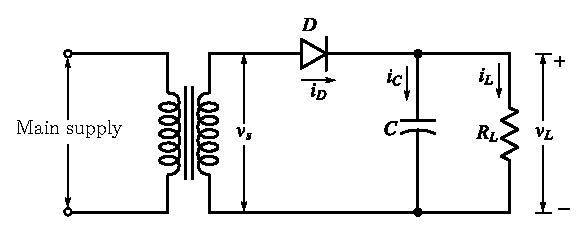
\includegraphics{chap1/fig1.37.eps}
\caption{Half-wave rectifier with capacitor filter}\label{fig1.37}
\end{figure}

Assume that the transformer secondary voltage $\upsilon_{\rms}$ is just starting to go positive from 0 volts and the capacitor is initially not charged. As the diode conducts, it charges $\rmC$ and $\upsilon_{\rmL}$ rises from $\rmt=0$ to $\rmt=\rmt_{1}$ as shown in Fig.~\ref{fig1.38}(b).

Beyond $\rmt_{1}$, $\upsilon_{\rmS}$ starts to drop, but the voltage across $\rmR_{\rmL}$ is prevented by the capacitor, following the same variation as $\upsilon_{\rmS}$. This is because the only way voltage across a capacitor can drop is to discharge. But here the reverse biased diode prevents the capacitor from discharging through the transformer secondary circuit and hence $\rmC$ can discharge only through $\rmR_{\rmL}$. To make $\rmC$ to discharge slowly between the time interval $\rmt_{1}$ and $\rmt_{2}$, both $\rmC$ and $\rmR_{\rmL}$ should be large i.e., the time constant $\rmR_{\rmL}\rmC$ should be large. But $\rmR_{\rmL}$ is fixed in value as this is the load to the circuit, only $\rmC$ can be chosen. By keeping the value of $\rmC$ large, the load voltage $\upsilon_{\rmL}$ can be made extremely smooth.

Fig.~\ref{fig1.38}(c) shows waveform of diode current $\rmi_{\rmD}$. During the interval between $\rmt=0$ and $\rmt=\rmt_{1}$, the diode current flows to deposit the initial charge on the capacitor $\rmC$. At $\rmt_{1}$, $\upsilon_{\rms}$ starts dropping below $\upsilon_{\rmL}$ and diode $\rmD$ is reverse biased. Thus, $\rmi_{\rmD}$ becomes zero. The zero diode current lasts at $\rmt=\rmt_{2}$ when $\upsilon_{\rmS}$ rises above $\upsilon_{\rmL}$. During the interval between $\rmt=\rmt_{1}$ and $\rmt=\rmt_{2}$, $\upsilon_{\rmL}$ drops as the capacitor $\rmC$ slowly discharges through $\rmR_{\rmL}$. As the time constant $\rmR_{\rmL}\rmC$ is large, the $\upsilon_{\rmL}$ decays very slowly between $\rmt=\rmt_{1}$ and $\rmt=\rmt_{2}$. The diode current $\rmi_{\rmD}$ pulse from $\rmt_{2}$ to $\rmt_{3}$ and each subsequent pulses are smaller in magnitude than the very first (i.e. between $\rmt=0$ and $\rmt=\rmt_{1}$). This is because at $\rmt=0$ the capacitor is uncharged while $\rmi_{\rmD}$ at $\rmt_{2}$, $\rmt_{4}$ etc., $\upsilon_{\rmL}$ is not much below the maximum value of $\upsilon_{\rms}$ i.e., $\rmV_{\rmm}$.
\begin{figure}[H]
\centering
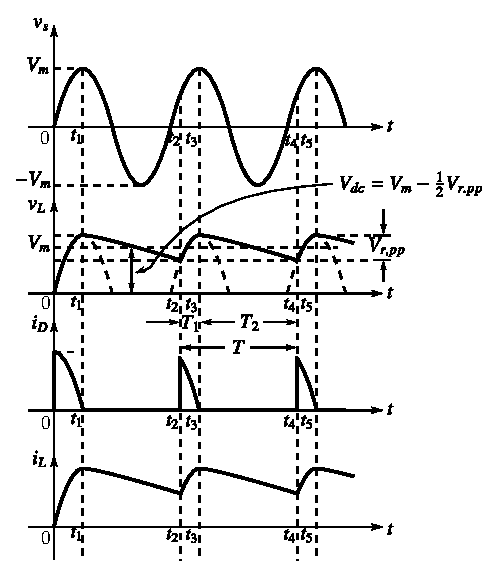
\includegraphics{chap1/fig1.38.eps}
\caption{Different waveforms of half-wave rectifier with capacitor filter}\label{fig1.38}
\end{figure}

\vskip -.4cm

Fig.~\ref{fig1.38}(d) shows waveform of the current $\rmi_{\rmL}$ through load $\rmR_{\rmL}$. Current through resistor always follows the voltage and hence $\rmi_{\rmL}$ is identical in shape to $\upsilon_{\rmL}$.

Now consider the load voltage $\upsilon_{\rmL}$ shown in Fig.~\ref{fig1.38}(b). This waveform follows a sinusoidal curvature during the charge period of capacitance (i.e., between $\rmt_{2}$ \&\ $\rmt_{3}$ and $\rmt_{4}$ \&\ $\rmt_{5}$ and so on). From $\rmt_{3}$ to $\rmt_{4}$ the load voltage $\upsilon_{\rmL}$ decays. This decay is actually exponential, but it can be considered as linear because only the initial small portion of the exponential curve is utilized. By approximating the waveform of load voltage $\upsilon_{\rmL}$ with straight line segments, the shape of it leads to sawtooth waveform. The charging time (eg. between $\rmt_{2}$ and $\rmt_{3}$) is very much smaller than the discharging time. (eg. between $\rmt_{3}$ and $\rmt_{4}$).

Fig.~\ref{fig1.39} shows the sawtooth approximation to ripple in the load voltage waveform $\upsilon_{\rmL}$.

The average or dc value of load current $\rmI_{\text{dc}}$ is the average value of the capacitor discharge current over period of $\rmT_{2}$. The amount of charge lost by the capacitor during the interval $\rmT_{2}$ is (refer Fig.~\ref{fig1.38}(b)).
\begin{equation}
\rmQ_{\text{discharge}} = \rmI_{\text{dc}}\times \rmT_{2}\label{eq1.30}
\end{equation}
\begin{figure}[H]
\centering
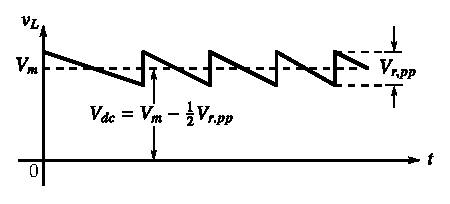
\includegraphics{chap1/fig1.39.eps}
\caption{Sawtooth approximation to ripple in the load voltage waveform \boldmath$\upsilon_{\rmL}$}\label{fig1.39}
\end{figure}



This charge is replaced during a short interval $\rmT_{1}$ during which the voltage across the capacitor changes by an amount equal to the peak-to-peak value of ripple, $\rmV_{\rmr,\text{pp}}$,
\begin{equation}
\text{i.e.,}\qquad \rmQ_{\text{charge}}=\rmV_{\rmr,\text{pp}}\times \rmC\label{eq1.31}
\end{equation}

We have
\begin{align}
\rmQ_{\text{charge}} &= \rmQ_{\text{discharge}}\notag\\[4pt]
\rmV_{\rmv,\text{pp}}\times \rmC &= \rmI_{\text{dc}}\times \rmT_{2}\notag\\[4pt]
\therefore\quad \rmV_{\text{r,pp}} &= \frac{\rmI_{\text{dc}}\times \rmT_{2}}{\rmC}\label{eq1.32}
\end{align}
But
\begin{equation}
\rmT_{2}\gg \rmT_{1}\quad\therefore\quad \rmT_{2}\simeq \rmT\simeq 1/f\label{eq1.33}
\end{equation}

Substituting Eqn.~\eqref{eq1.33} into Eqn.~\eqref{eq1.32}, we get
\begin{align}
\rmV_{\text{r,pp}} &= \frac{\rmI_{\text{dc}}\times \rmT}{\rmC}\notag\\[4pt]
\rmV_{\text{r,pp}} &= \frac{\rmI_{\text{dc}}}{f\rmC}\label{eq1.34}
\end{align}

The rms value of sawtooth waveform with peak-to-peak value $\rmV_{\text{r,pp}}$ is given by
\begin{align}
\rmV_{\text{r,rms}} &= \frac{\rmV_{\text{r,pp}}}{2\sqrt{3}}\notag\\[4pt]
\therefore\quad \rmV_{\text{r,pp}} &= 2\sqrt{3}\cdot \rmV_{\text{r,rms}}\label{eq1.35}
\end{align}

Also we have
\begin{equation}
\rmI_{\text{dc}}=\frac{\rmV_{\text{dc}}}{\rmR_{\rmL}}\label{eq1.36}
\end{equation}

Substituting Eqn.~\eqref{eq1.35} and \eqref{eq1.36} in Eqn.~\eqref{eq1.34}, we get,
\begin{align}
2\sqrt{3}\rmV_{\text{r,rms}} &= \frac{\rmV_{\text{dc}}}{f\rmR_{\rmL}\rmC}\notag\\[4pt]
\therefore\quad \text{ripple factor~ } \rmr &= \frac{\rmV_{\text{r,rms}}}{\rmV_{\text{dc}}}\notag\\[4pt]
\rmr &= \frac{1}{2\sqrt{3}f\rmR_{\rmL}\rmC}\label{eq1.37}
\end{align}

Thus, as the load resistor $\rmR_{\rmL}$ increases, the ripple factor decreases. Therefore the capacitor filter is better for light load (i.e. large $\rmR_{\rmL}$).

From Fig.~\ref{fig1.38}(b) we have,
\begin{equation}
\rmV_{\text{dc}}=\rmV_{\rmm}=\dfrac{\rmV_{\text{r,pp}}}{2}\label{eq1.38}
\end{equation}

Substituting Eqn.~\eqref{eq1.34} in Eqn.~\eqref{eq1.38}, we get
\begin{equation}
\rmV_{\text{dc}}=\rmV_{\rmm}-\dfrac{\rmI_{\text{dc}}}{2f\rmC}\label{eq1.39}
\end{equation}

Substituting Eqn.~\eqref{eq1.36} in Eqn.~\eqref{eq1.39}, we get
\begin{align}
\rmV_{\text{dc}} &= \rmV_{\rmm}-\dfrac{\rmV_{\text{dc}}}{2f\rmR_{\rmL}\rmC}\notag\\[4pt]
\therefore\quad \rmV_{\text{dc}} &= \left[\frac{2f\rmR_{\rmL}\rmC}{1+2f\rmR_{\rmL}\rmC}\right]\rmV_{\rmm}\label{eq1.40}
\end{align}
Thus the output dc voltage can be increased by increasing $\rmR_{\rmL}$ or $\rmC$.

\begin{center}
\rule{4cm}{1pt}\\
{\bf\Large Problems}\\[-3pt]
\rule{4cm}{1pt}
\end{center}

\begin{problem}\label{prob1.17}
In a half-wave rectifier circuit fed from 230 V, 50 Hz mains, it is desired to have a ripple factor $\rmr<0.005$. Find the value of the capacitance needed to get dc load current of 500 mA. Assume diode is ideal.
\end{problem}

\begin{solution}
Given
\begin{align*}
\rmI_{\text{dc}} &= 500 \text{~mA}, \ r<0.005, \ f=50\text{~Hz}.\\[3pt]
\rmV_{\rmm} &= \sqrt{2}\times 230=325.3\rmV
\end{align*}
We have
\begin{align}
\rmV_{\text{dc}} &= \left[\frac{2f\rmR_{\rmL}\rmC}{1+2f\rmR_{\rmL}\rmC}\right]\rmV_{\rmm}\label{eq1.41}\\[4pt]
\text{ripple factor~~ } \rmr &= \frac{1}{2\sqrt{3}f\rmR_{\rmL}\rmC}\notag\\[3pt]
\therefore\quad 2f\rmR_{\rmL}\rmC &= \frac{1}{\sqrt{3}.\rmr}\notag\\[3pt]
 &= \frac{1}{\sqrt{3}\times 0.005}\notag\\[3pt]
2f\rmR_{\rmL}\rmC &= 115.47\label{eq1.42}
\end{align}

Substituting Eqn.~\eqref{eq1.42} in Eqn.~\eqref{eq1.41}, we get
\begin{align*}
\rmV_{\text{dc}} &= \frac{115.47}{(1+115.47)}\times 325.3\\[4pt]
&= 322.5\rmV\\[3pt]
\therefore~ \text{Load resistor~~ } \rmR_{\rmL} = \frac{\rmV_{\text{dc}}}{\rmI_{\text{dc}}} &= \frac{322.5}{500\times 10^{-3}}=645\simeq 650\Omega\\[3pt]
\rmr &= \frac{1}{2\sqrt{3}f\rmR_{\rmL}\rmC}\\[3pt]
0.005 &< \frac{1}{2\sqrt{3}f\rmR_{\rmL}\rmC}\\[3pt]
\therefore\quad \rmC &> \frac{1}{2\sqrt{3}f\rmR_{\rmL}(0.005)}\\[3pt]
\rmC &> \frac{1}{2\sqrt{3}(50)(650)(0.005)}\\[3pt]
\rmC &> 1.776\text{~mF}\quad\therefore\quad \text{Select~ } \rmC=1.8\text{~ mF}
\end{align*}
\end{solution}

\begin{problem}\label{prob1.18}
A half-wave rectifier using a capacitor filter is to supply 30 Vdc to a 1k$\Omega$ load. Assuming the diode forward resistance is negligible, calculate the input voltage required and the value of filter capacitor for a ripple of 0.03.
\end{problem}

\begin{solution}
Given~:~ $\rmV_{\text{dc}}=30\rmV$, \ $\rmR_{\rmL}=1\rmk\Omega$, $\rmr=0.03$. Assume $f=50$ Hz.

DC load current $\rmI_{\text{dc}}=\dfrac{\rmV_{\text{dc}}}{\rmR_{\rmL}}=\dfrac{30}{1\times 10^{3}}=30$~mA

We have
\begin{equation}
\rmV_{\text{dc}}=\left[\frac{2f\rmR_{\rmL}\rmC}{1+2f\rmR_{\rmL}\rmC}\right]\rmV_{\rmm}\quad\text{and}\quad r=\dfrac{1}{2\sqrt{3}f\rmR_{\rmL}\rmC}\label{eq1.43}
\end{equation}
$\therefore$~ Required \ $\rmC=\dfrac{1}{2\sqrt{3}f\rmR_{\rmL}\rmr}=\dfrac{1}{2\sqrt{3}\times 50\time 1\times 10^{3}\times 0.03}=193\mu\rmF$
\begin{equation}
\therefore\quad 2f\rmR_{\rmL}\rmC=\dfrac{1}{\sqrt{3}\times \rmr}=\dfrac{1}{\sqrt{3}\times 0.03}=19.25\label{eq1.44}
\end{equation}

Substituting Eqn.~\eqref{eq1.44} in Eqn.~\eqref{eq1.43}, we get
\begin{align*}
\rmV_{\text{dc}} &= \frac{19.25}{(1+19.25)}\cdot \rmV_{\rmm}\\[3pt]
\rmV_{\text{dc}} &= 0.9505\rmV_{\rmm}\\[3pt]
\rmV_{\rmm} &= \frac{\rmV_{\text{dc}}}{0.9506}=\dfrac{30}{0.9506}=31.56\rmV
\end{align*}
$\therefore$~ rms voltage required across the secondary of the transformer
\begin{align*}
&= \rmV_{\rmm}/\sqrt{2}\\[3pt]
&= 31.56/\sqrt{2}\\[3pt]
&= 22.32\rmV
\end{align*}
\end{solution}


\subsection{Full-wave rectifier with capacitor filter}\label{sec1.11.2}

A full-wave rectifier with capacitor filter is shown in Fig.~\ref{fig1.40}.
\begin{figure}[H]
\centering
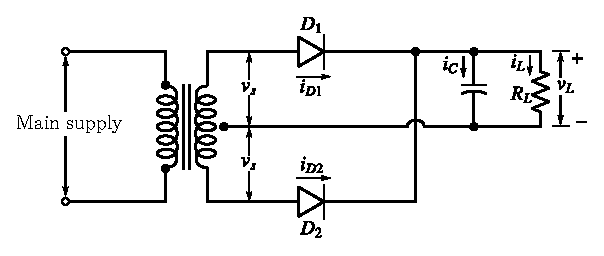
\includegraphics{chap1/fig1.40.eps}
\caption{Full-wave rectifier with capacitor filter}\label{fig1.40}
\end{figure}

The working of full-wave rectifier with capacitor filter is same as that of halfwave rectifier with capacitor. But here we get 2 output cycles for each input cycle. The different waveforms are shown in Fig.~\ref{fig1.40}.

The average or dc value of load current $\rmI_{\text{dc}}$ is the average value of the capacitor discharge current over period $\rmT_{2}$. The amount of charge lost by the capacitor during the interval $\rmT_{2}$ is, (refer Fig.~\ref{fig1.38}(b))
\begin{equation}
\rmQ_{\text{discharge}}=\rmI_{\text{dc}}\times \rmT_{2}\label{eq1.45}
\end{equation}

This charge is replaced during a short interval $\rmT_{1}$ during which the voltage across the capacitor changes by an amount equal to the peak-to-peak value of ripple, i.e., $\rmV_{\text{r,pp}}$.
\begin{equation}
\therefore\quad \rmQ_{\text{charge}}=\rmV_{\text{r,pp}}\times C\label{eq1.46}
\end{equation}
We have
\begin{align}
\rmQ_{\text{charge}} &= \rmQ_{\text{discharge}}\notag\\[3pt]
\rmV_{\text{r,pp}}\times \rmC &= \rmI_{\text{dc}}\times \rmT_{2}\notag\\[3pt]
\therefore\quad \rmV_{\text{r,pp}} &= \frac{\rmI_{\text{dc}}\times \rmT_{2}}{\rmC}\label{eq1.47}
\end{align}
But
\begin{equation}
\rmT_{2}\gg \rmT_{1}\quad\therefore\quad \rmT_{2}\simeq \dfrac{\rmT}{2}=\frac{1}{2f}\label{eq1.48}
\end{equation}
Substituting Eqn.~\eqref{eq1.48} in Eqn.~\eqref{eq1.47}, we get
\begin{align}
\rmV_{\text{r,pp}} &= \dfrac{\rmI_{\text{dc}}\times \rmT}{1\rmC}\notag\\[3pt]
\rmV_{\text{r,pp}} &= \frac{\rmI_{\text{dc}}}{2f\rmC}\label{eq1.49}
\end{align}

The output load voltage $\upsilon_{\rmL}$ can be approximated to sawtooth waveform.

The rms value of sawtooth waveform with peak-to-peak value $\rmV_{\text{r,pp}}$ is given by
\begin{align}
\rmV_{\text{r,rms}} &= \frac{\rmV_{\text{r,pp}}}{2\sqrt{3}}\notag\\[3pt]
\therefore\quad \rmV_{\text{r,pp}} &= 2\sqrt{3}\cdot \rmV_{\text{r,rms}}\label{eq1.50}\\[3pt]
\text{Also we have~~ } \rmI_{\text{dc}} &= \frac{\rmV_{\text{dc}}}{\rmR_{\rmL}}\label{eq1.51}
\end{align}
Substituting Eqn.~\eqref{eq1.50} and \eqref{eq1.51} in Eqn.~\eqref{eq1.49}, we get,
$$
2\sqrt{3}\rmV_{\text{r,rms}} = \frac{\rmV_{\text{dc}}}{2f\rmR_{\rmL}\rmC}
$$
\begin{figure}[H]
\centering
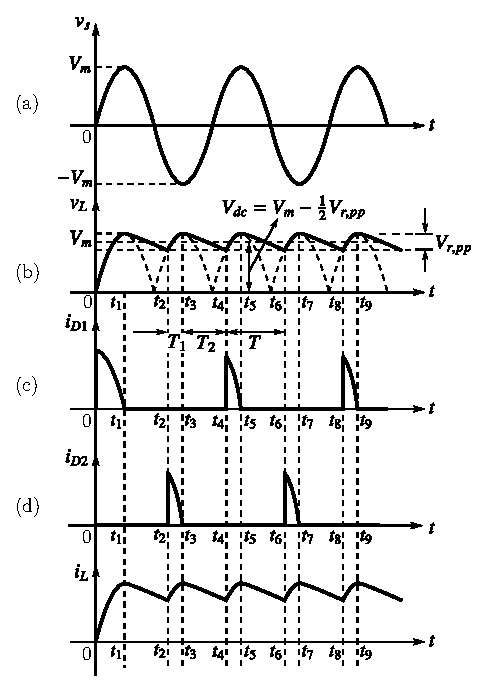
\includegraphics{chap1/fig1.41.eps}
\caption{}\label{fig1.41}
\end{figure}

We have,
\begin{align}
\text{ripple factor~~ } \rmr &= \frac{\rmV_{\text{r,rms}}}{\rmV_{\text{dc}}}\notag\\[3pt]
\therefore\quad \rmr &= \frac{1}{4\sqrt{3}f\rmR_{\rmL}\rmC}\label{eq1.52}
\end{align}
From Fig.~\ref{fig1.38}(b) we have,
\begin{equation}
\rmV_{\text{dc}}=\rmV_{\rmm}-\frac{\rmV_{\text{r,pp}}}{2}\label{eq1.53}
\end{equation}
Substituting Eqn.~\eqref{eq1.49} in Eqn.~\eqref{eq1.53}, we get
\begin{equation}
\rmV_{\text{dc}}=\rmV_{\rmm}-\frac{\rmI_{\text{dc}}}{4f\rmC}\label{eq1.54}
\end{equation}
Substituting Eqn.~\eqref{eq1.51} in Eqn.~\eqref{eq1.54}, we get,
\begin{align}
\rmV_{\text{dc}} &= \rmV_{\rmm} - \frac{\rmV_{\text{dc}}}{4f\rmR_{\rmL}\rmC}\notag\\[3pt]
\therefore\quad \rmV_{\text{dc}} &= \left[\frac{4f\rmR_{\rmL}\rmC}{1+4f\rmR_{\rmL}\rmC}\right]\rmV_{\rm}\label{eq1.55}
\end{align}
Thus the output dc voltage can be increased by increasing $\rmR_{\rmL}$ or $\rmC$.

\begin{note}
The waveforms and equations which are described for centre-tapped transformer full-wave rectifier with capacitor filter are also valid for full-wave bridge rectifier with capacitor filter.
\end{note}

\begin{center}
\rule{4cm}{1pt}\\
{\bf\Large Problems}\\[-3pt]
\rule{4cm}{1pt}
\end{center}

\begin{problem}\label{prob1.1}
Find the dc voltage that can be obtained from the full wave rectifier shown in Fig.~\ref{fig1.42}. Assume $\rmR_{\rmf}=0\Omega$
\begin{itemize}
\item[(a)] without capacitor filter

\item[(b)] with capacitor filter $\rmC=1000\mu\rmF$.
\begin{figure}[H]
\centering
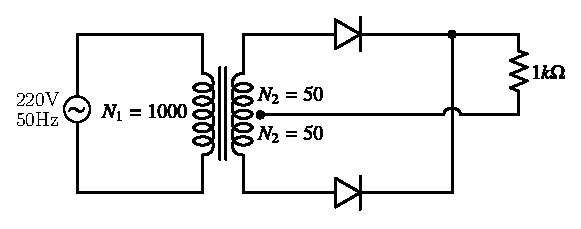
\includegraphics{chap1/fig1.42.eps}
\caption{}\label{fig1.42}
\end{figure}
\end{itemize}
\end{problem}

\begin{solution}
Given~:~ $f=50$ HZ, \ $\rmN_{1}=1000$, \ $\rmN_{2}=50$, \ $\rmR_{\rmL}=1\; \rmk\Omega$.

\vskip .1cm
The rms voltage across the primary = 220 V.

\vskip .1cm
$\therefore$~ The rms voltage across half winding of the secondary $=220\times {}^{50}/1000=11\rmV$.

\vskip .1cm
$\therefore$~ Maximum voltage $\rmV_{\rmm}=\sqrt{2}\times 11=15.56\rmV$.
\begin{itemize}
\item[(a)] Without capacitor filter~:
\begin{align*}
\text{Maximum load current~~ } \rmI_{\rmm} &= \frac{\rmV_{\rmm}}{\rmR_{\rmf}+\rmR_{\rmL}}\\[4pt]
&= \dfrac{15.56}{1\times 10^{3}}\qquad [\because \ \rmR_{\rmf}=0\Omega]\\[3pt]
&= 15.56\text{~mA}
\end{align*}
\begin{align*}
\therefore \ \text{dc load current~ } \rmI_{\text{dc}} &= \frac{2\rmI_{\rmm}}{\pi}\\[4pt]
&= \frac{2\times 15.56\times 10^{-3}}{\pi}\\[4pt]
&= 9.91\text{~mA}\\[3pt]
\therefore~ \text{dc output voltage~ } \rmV_{\text{dc}} &= \rmI_{\text{dc}}\cdot \rmR_{\rmL}\\[3pt]
&= (9.91\times 10^{-3})(1\times 10^{3})\\[3pt]
&= 9.91\rmV
\end{align*}

\item[(b)] With capacitor filter~:

Given~:
\begin{align*}
\rmC &= 1000 \mu\rmF\\[3pt]
\rmV_{\text{dc}} &= \left[\frac{4f\rmR_{\rmL}\rmC}{1+4f\rmR_{\rmL}\rmC}\right]\rmV_{\rmm}\\[3pt]
&= \left[\frac{4\times 50\times 1\times 10^{3}\times 1000\times 10^{-6}}{1+4\times 50\times 1\times 10^{3}\times 1000\times 10^{-6}}\right]\times 15.56\\[3pt]
\rmV_{\text{dc}} &= 15.48\rmV
\end{align*}
\end{itemize}
\end{solution}

\begin{problem}\label{prob1.20}
A 220 V, 50 Hz input is applied to a bridge rectifier with load 500 $\Omega$. Calculate the output dc voltage, dc load current and ripple factor.
\begin{itemize}
\item[(a)] Without capacitor filter

\item[(b)] With capacitor filter $\rmC=1000\mu\rmF$.
\end{itemize}
Assume diodes are ideal.
\end{problem}

\begin{solution}
Given \ $\rmV_{\text{rms}}=220\rmV$, \ $f=50$ Hz, \ $\rmR_{\rmL}=500\Omega$.
\begin{align*}
\therefore ~ \text{~ Maximum voltage } \rmV_{\rmm} &= \sqrt{2}\times 220\\[3pt]
          &= 311.13\rmV
\end{align*}
\begin{itemize}
\item[(a)] Without capacitor filter
\begin{align*}
\text{Peak current~~ } \rmI_{\rmm} &= \frac{\rmV_{\rmm}}{2\rmR_{\rmf}+\rmR_{\rmL}}\qquad [\because \ \rmR_{\rmf}=0\Omega]\\[3pt]
&= \frac{311.13}{500}\\[3pt]
&= 622.3\text{~ mA}\\[3pt]
\therefore\quad \text{dc load current~~ } \rmI_{\text{dc}} &= \frac{2\rmI_{\rmm}}{\pi}=\dfrac{2\times 622.3\times 10^{-3}}{\pi}\\[3pt]
&= 396.17\text{~mA}\\[3pt]
\therefore\quad \text{output dc voltage~~ } \rmV_{\text{dc}} &= \rmI_{\text{dc}}\cdot \rmR_{\rmL}\\[3pt]
&= 396.17\times 10^{-3}\times 500\\[3pt]
&= 198.1\rmV\\[3pt]
\text{ripple factor~~ } \rmr &= 0.483\quad [\because \ \rmR_{\rmf}=0\Omega]
\end{align*}

\item[(b)] With capacitor filter : $\rmC=1000\mu\rmF$
\begin{align*}
\text{dc output voltage~~ } \rmV_{\text{dc}} &= \left[\frac{4f\rmR_{\rmL}\rmC}{1+4f\rmR_{\rmL}\rmC}\right]\cdot \rmV_{\rmm}\\[3pt]
&= \left[\frac{4\times 50\times 500\times 1000\times 10^{-6}}{1+4\times 50\times 500\times 1000\times 10^{-6}}\right]\times 311.13\\[3pt]
\rmV_{\text{dc}} &= 308.1\rmV\\[3pt]
\therefore\quad \text{dc load current~~ } \rmI_{\text{dc}} &= \frac{\rmV_{\text{dc}}}{\rmR_{\rmL}}=\dfrac{308.1}{500}=616.1\text{~mA}\\[3pt]
\text{ripple factor~~ } \rmr &= \frac{1}{4\sqrt{3}f\rmR_{\rmL}\rmC}\\[3pt]
&= \frac{1}{4\times \sqrt{3}\times 50\times 500\times 1000\times 10^{-6}}\\[3pt]
&\simeq 0.0058
\end{align*}
\end{itemize}
\end{solution}

\begin{problem}\label{prob1.21}
A full-wave rectifier with $1000\mu\rmF$ capacitor across load resistor has maximum input voltage of $10\rmV$ at 50 Hz and the peak to peak ripple voltage of 0.1 V. Find the dc load current.
\end{problem}

\begin{solution}
Given~: $\rmV_{\rmm}=10\rmV$, \ $f=50$ Hz, \ $\rmV_{\text{r,pp}}=0.1\rmV$
\begin{align*}
\therefore\quad \text{dc output voltage~~ } \rmV_{\text{dc}} &= \rmV_{\rmm}-\frac{1}{2}\rmV_{\text{r,pp}}\\[4pt]
&= 10-\frac{1}{2}\times 0.1\\[4pt]
&= 9.95\rmV
\end{align*}
The rms value of ripple voltage is,
\begin{align*}
\rmV_{\text{r,rms}} &= \frac{\rmV_{\text{r,pp}}}{2\sqrt{3}}=\dfrac{0.1}{2\times \sqrt{3}}=0.0289\rmV\\[3pt]
\therefore\quad \text{ripple factor~~ } \rmr &= \frac{\rmV_{\text{r,rms}}}{\rmV_{\text{dc}}}=\dfrac{0.0289}{9.95}=0.0029
\end{align*}
Also we have, ripple factor $\rmr=\dfrac{1}{4\sqrt{3}f\rmR_{\rmL}\rmC}$
\begin{align*}
\therefore\quad \text{load resistor~~ } \rmR_{\rmL} &= \frac{1}{4\sqrt{3}f\rmC\rmr}\\[3pt]
&= \frac{1}{4\sqrt{3}\times 50\times 1000\times 10^{-6}\times 0.0029}\\[3pt]
&= 995\Omega\\[3pt]
\therefore\quad \text{dc load current~~ } \rmI_{\text{dc}} &= \frac{\rmV_{\text{dc}}}{\rmR_{\rmL}}=\dfrac{9.95}{995}\simeq 10\text{~mA}
\end{align*}
\end{solution}

\begin{problem}\label{prob1.22}
Consider a bridge rectifier circuit with capacitor filter which has transformer turns ratio $2.3:1$, $\rmR_{\rmL}=500\Omega$ and $\rmC=1000\mu\rmF$. If the rms input voltage to the transformer primary is 115 V, 60 Hz, determine
\begin{itemize}
\item[(a)] rms ripple voltage

\item[(b)] dc load voltage

\item[(c)] dc load power
\end{itemize}
\end{problem}

\begin{solution}
Given~: $\rmR_{\rmL}=500\Omega$,  \ $\rmC=1000\mu\rmF$, \ $f=60$ Hz, \ $\rmN_{1}:\rmN_{2}=2.3:1$;

The rms voltage across transformer primary = 115 V

\begin{tabbing}
$\therefore$~ The rms voltage across the secondary of transformer \== $115\times \dfrac{1}{2.3}$\\[5pt]
\>= 50 V
\end{tabbing}
\begin{align*}
\text{Maximum voltage~~} \rmV_{\rmm} &= \sqrt{2}\times 50=70.7\rmV\\[3pt]
\therefore~~ \text{dc load voltage~~ } \rmV_{\text{dc}} &= \left[\frac{4f\rmR_{\rmL}\rmC}{1+4f\rmR_{\rmL}\rmC}\right]\rmV_{\rmm}\\[3pt]
&= \left[\frac{4\times 60\times 500\times 1000\times 10^{-6}}{1+4\times 60\times 500\times 1000\times 10^{-6}}\right]\times 70.7\\[3pt]
\rmV_{\text{dc}} &= 70.116\rmV
\end{align*}
We have
\begin{align*}
\rmV_{\text{dc}} &= \rmV_{\rmm}-\frac{1}{2}\rmV_{\text{r,pp}}\\[3pt]
\rmV_{\text{r,pp}} &= 2[\rmV_{\rmm}-\rmV_{\text{dc}}]\\[3pt]
&= 2(70.7-70.116)\\[3pt]
\rmV_{\text{r,pp}} &= 1.169\rmV
\end{align*}
$\therefore$~ rms value of ripple voltage
\begin{align*}
\rmV_{\text{r,rms}} &= \frac{\rmV_{\text{r,pp}}}{2\sqrt{3}}=\dfrac{1.169}{2\sqrt{3}}=0.337\rmV\\[3pt]
\therefore\quad \text{dc load current~~ } \rmI_{\text{dc}} &= \frac{\rmV_{\text{dc}}}{\rmR_{\rmL}}=\dfrac{70.116}{500}=140.2\text{~mA}\\[3pt]
\therefore\quad \text{dc load power~~ } \rmP_{\text{dc}} &= \rmV_{\text{dc}}\rmI_{\text{dc}}\\[3pt]
&= 70.116\times 140.2\times 10^{-3}\\[3pt]
\rmP_{\text{dc}} &= 9.83\rmW
\end{align*}
\begin{itemize}
\item[(a)] rms ripple voltage $\rmV_{\text{r,rms}}=0.337\rmV$

\item[(b)] dc load voltage $\rmV_{\text{dc}}=70.116\rmV$

\item[(c)] dc load power $\rmP_{\text{dc}}=9.83\rmW$
\end{itemize}
\end{solution}

\begin{problem}\label{prob1.23}
The output voltage waveform of a full-wave rectifier with load $\rmR_{\rmL}=100\Omega$, and a filter capacitor $\rmC=1050\mu\rmF$ is shown in Fig.~\ref{fig1.43}. The power line frequency is 60 Hz. Find the ripple factor, the dc output voltage and peak-to-peak ripple voltage.
\begin{figure}[H]
\centering
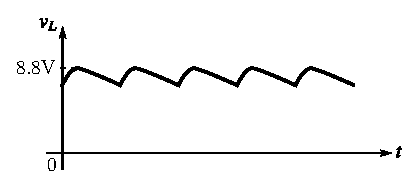
\includegraphics{chap1/fig1.43.eps}
\caption{}\label{fig1.43}
\end{figure}
\end{problem}

\begin{solution}
Given \ \ $f=60$\,Hz.

\vskip .1cm
From Fig.~\ref{fig1.43}, we have, $\rmV_{\rmm}=8.8\rmV$
\begin{align*}
\therefore\quad \text{dc load voltage~~ } \rmV_{\text{dc}} &= \left[\frac{4f\rmR_{\rmL}\rmC}{1+4f\rmR_{\rmL}\rmC}\right]\rmV_{\rmm}\\[3pt]
&= \left[\frac{4\times 60\times 100\times 1050\times 10^{-6}}{1+4\times 60\times 100\times 1050\times 10^{-6}}\right]\times 8.8\\[3pt]
&= 8.46\rmV\\[3pt]
\text{ripple factor~~ }\rmr &= \frac{1}{4\sqrt{3}f\rmR_{\rmL}\rmC}\\[3pt]
&=\frac{1}{4\sqrt{3}\times 60\times 100\times 1050\times 10^{-6}}\\[3pt]
\rmr &= 0.0229
\end{align*}
We have ripple factor \ $\rmr=\dfrac{\rmV_{\text{r,rms}}}{\rmV_{\text{dc}}}$
\begin{align*}
\therefore\quad \rmV_{\text{r,rms}} &= \rmr\times \rmV_{\text{dc}}\\[3pt]
&= 0.0229\times 8.46\\[3pt]
&= 0.194\rmV
\end{align*}
We have~~ $\rmV_{\text{r,rms}}=\dfrac{\rmV_{\text{r,pp}}}{2\sqrt{3}}$.

\eject

\begin{tabbing}
$\therefore$\quad Peak-to-peak ripple voltage \ \ $\rmV_{\text{r,pp}}$ \== $2\sqrt{3}\rmV_{\text{r,rms}}$\\[4pt]
\>= $2\sqrt{3}\times 0.194$\\[4pt]
\>= $0.67\rmV$
\end{tabbing}
\end{solution}

\begin{problem}\label{prob1.24}
A load is to be supplied 10 mA at 50 Vdc with a ripple not more than 2\%. Calculate the value of the filter capacitor that would be needed for a full-wave bridge rectifier circuit.

Main source voltage is 220V, 50 Hz. Also calculate transformer turns ratio.
\end{problem}

\begin{solution}
Given : $\rmI_{\text{dc}}=10$ mA, \ $\rmV_{\text{dc}}=50$ V, \ $\rmr<0.02$, \ $f=50$ Hz
$$
\text{Load resistor ~~ } \rmR_{\rmL} =\dfrac{\rmV_{\text{dc}}}{\rmI_{\text{dc}}}=\dfrac{50}{10\times 10^{-3}}=5\rmk\Omega
$$
We have
\begin{align*}
\rmr &= \frac{1}{4\sqrt{3}f\rmR_{\rmL}\rmC}\\[3pt]
\rmr &< \dfrac{1}{4\sqrt{3}f\rmR_{\rmL}\rmC}\\[3pt]
\therefore\quad \rmC &> \dfrac{1}{4\sqrt{3}f\rmR_{\rmL}\rmr}\\[3pt]
\rmC &> \dfrac{1}{4\sqrt{3}\times 50\times 5\times 10^{3}\times 0.02}\\[3pt]
\rmC &> 28.87\mu\rmF\\[3pt]
\therefore\quad \text{Select~~ } \rmC &= 30\mu\rmF
\end{align*}
We have
\begin{align*}
\rmV_{\text{dc}} &= \left[\frac{4f\rmR_{\rmL}\rmC}{1+4f\rmR_{\rmL}\rmC}\right]\cdot \rmV_{\rmm}\\[3pt]
\therefore\quad \text{Peak voltage~~ }\rmV_{\rmm} &= \rmV_{\text{dc}}\left[\frac{1+4f\rmR_{\rmL}\rmC}{4f\rmR_{\rmL}\rmC}\right]\\[3pt]
&= 50 \left[\frac{1+4\times 50\times 5\times 10^{3}\times 30\times 10^{-6}}{4\times 50\times 5\times 10^{3}\times 30\times 10^{-6}}\right]
\end{align*}
$\therefore$~~ The maximum voltage required across the secondary of the transformer
$$
\rmV_{\rmm}=51.67\rmV
$$
Given the rms voltage across the primary of the transformer = 220 V

\vfill\eject

$\therefore$~~ the maximum voltage across the primary of the transformer
$$
=\sqrt{2}\times 220=311.13\rmV
$$

$\therefore$~~ the turns ratio of the transformer is,
\begin{align*}
\frac{\rmN_{1}}{\rmN_{2}} &= \frac{311.13}{51.67}\\[4pt]
\therefore\quad \rmN_{1}:\rmN_{2} &= 6:1
\end{align*}
\end{solution}

\begin{problem}\label{prob1.25}
A full-wave rectifier with a $120\mu\rmF$ capacitor filter connected to a load of 60 mA. If the peak voltage of the rectified wave is 60 V, calculate.
\begin{itemize}
\item[(a)] the dc output voltage\qquad (b) the ripple voltage\qquad (c) the ripple factor.
\end{itemize}
Given that frequency of source = 50 Hz.
\end{problem}

\begin{solution}
$\rmV_{\rmm}=60\rmV$, \ $f=50$ Hz, \ $\rmI_{\text{dc}}=60$ mA, \ $\rmC=120 \ \mu\rmF$.

\vskip .1cm
We have
\begin{align}
\text{ripple factor~~ } \rmr &= \frac{1}{4\sqrt{3}f\rmR_{\rmL}\rmC}=\dfrac{\rmV_{\text{r,rms}}}{\rmV_{\text{dc}}}\label{eq1.56}\\[3pt]
\text{Also}\qquad \rmR_{\rmL} &= \frac{\rmV_{\text{dc}}}{\rmI_{\text{dc}}}\label{eq1.57}
\end{align}
Substituting Eqn.~\eqref{eq1.57} in Eqn.~\eqref{eq1.56}, we get
\begin{align*}
\frac{\rmI_{\text{dc}}}{4\sqrt{3}f\rmV_{\text{dc}}\cdot \rmC} &= \frac{\rmV_{\text{r,rms}}}{\rmV_{\text{dc}}}\\[4pt]
\therefore\quad \rmV_{\text{r,rms}} &= \frac{\rmI_{\text{dc}}}{4\sqrt{3}f\rmC}\\[4pt]
&= \frac{60\times 10^{-3}}{4\sqrt{3}\times 50\times 120\times 10^{-6}}\\[4pt]
\rmV_{\text{r,rms}} &= 1.44\rmV\\[4pt]
\text{We have,}\qquad \rmV_{\text{r,rms}} &= \frac{\rmV_{\text{r,pp}}}{2\sqrt{3}}
\end{align*}

\eject

$\therefore$~ Peak-to-peak ripple voltage
\begin{align*}
\rmV_{\text{r,pp}} &= 2\sqrt{3}\cdot \rmV_{\text{r,rms}}\\[3pt]
&= 2\sqrt{3}\times 1.44\\[3pt]
\rmV_{\text{r,pp}} &= 5\rmV
\end{align*}
$\therefore$~ dc output voltage
\begin{align*}
\rmV_{\text{dc}} &= \rmV_{\rmm}-\dfrac{1}{2}\rmV_{\text{r,pp}}\\[3pt]
              &= 60-\frac{1}{2}\times 5\\[3pt]
\rmV_{\text{dc}} &= 57.5\rmV
\end{align*}
$\therefore$~~ ripple factor \ \ $\rmr=\dfrac{\rmV_{\text{r,rms}}}{\rmV_{\text{dc}}}=\dfrac{1.44}{57.5}=0.025$
\begin{itemize}
\item[(a)] the dc output voltage \ \ $\rmV_{\text{dc}}=57.5\rmV$

\item[(b)] the ripple voltage $\rmV_{\text{r,pp}}=5\rmV$

\item[(c)] the ripple factor \ $\rmr=0.025$
\end{itemize}
\end{solution}

\begin{problem}\label{prob1.26}
A full-wave rectifier supplies a load of $10\rmk\Omega$. The ac voltage applied to the diode is 300-0-300 $\rmV_{\text{rms}}$ with frequency 50 Hz. If the diode resistance is neglected, calculate (a) $\rmV_{\text{dc}}$ \ \ (b) $\rmI_{\text{dc}}$ \ \ (c) ripple voltage
\begin{itemize}
\item[(i)] without capacitor filter

\item[(ii)] with capacitor filter $(\rmC=2000\mu\rmF)$
\end{itemize}
\end{problem}

\begin{solution}
Given~:~ $\rmR_{\rmL}=10\rmk\Omega$, \ \ $f=50$Hz.

Supply to the full-wave rectifier = 300 $\rmV_{\text{rms}}$

$\therefore$~~ Maximum voltage $\rmV_{\rmm}=\sqrt{2}\times 300=424.3\rmV$
\begin{itemize}
\item[(i)] without capacitor filter
\begin{align*}
\rmV_{\text{dc}} &= \frac{2\rmV_{\rmm}}{\pi}=\dfrac{2\times 424.3}{\pi}=270\rmV\\[3pt]
\rmI_{\text{dc}} &= \frac{\rmV_{\text{dc}}}{\rmR_{\rmL}}=\dfrac{270}{10\times 10^{3}}=27\text{~mA}
\end{align*}
Since diode is ideal, ripple factor \ $\rmr=0.481$.

We have\quad $\rmr=\dfrac{\rmV_{\text{r,rms}}}{\rmV_{\text{dc}}}$
\begin{align*}
\therefore\quad \text{rms ripple voltage~~ }\rmV_{\text{r,rms}} &= \rmr\times \rmV_{\text{dc}}\\[3pt]
&= 0.481\times 270\\[3pt]
&= 129.9\rmV
\end{align*}

\item[(ii)] with capacitor filter : $\rmC=2000\mu\rmF$.
\begin{align*}
\rmV_{\text{dc}} &= \left[\frac{4f\rmR_{\rmL}\rmC}{1+4f\rmR_{\rmL}\rmC}\right]\cdot \rmV_{\rmm}\\[3pt]
&= \left[\frac{4\times 50\times 10\times 10^{3}\times 2000\times 10^{-6}}{1+4\times 50\times 10\times 10^{3}\times 2000\times 10^{-6}}\right]\times 424.3\\[3pt]
\rmV_{\text{dc}} &= 424.2\rmV\\[3pt]
\therefore\quad \rmI_{\text{dc}} &= \frac{\rmV_{\text{dc}}}{\rmR_{\rmL}}=\dfrac{424.2}{10\times 10^{3}}=42.42\text{~mA}\\[3pt]
\text{ripple factor~ } &= \frac{1}{4\sqrt{3}f\rmR_{\rmL}\rmC}\\[3pt]
&= \frac{1}{4\sqrt{3}\times 50\times 10\times 10^{3}\times 2000\times 10^{-6}}\\[3pt]
&= 0.00014
\end{align*}
Also, \ \ $\rmr=\dfrac{\rmV_{\text{r,rms}}}{\rmV_{\text{dc}}}$
\begin{align*}
\therefore\quad \rmV_{\text{r,rms}} &= \rmr\times \rmV_{\text{dc}}\\[3pt]
&= 0.00014\times 424.2\\[3pt]
&= 0.06\rmV
\end{align*}
Peak-to-peak ripple voltage
\begin{align*}
\rmV_{\text{r,pp}} &= 2\sqrt{3}\cdot \rmV_{\text{r,rms}}\\[3pt]
                &= 2\sqrt{3}\times 0.06\\[3pt]
\rmV_{\text{r,pp}} &= 0.208\rmV
\end{align*}
\end{itemize}
\end{solution}

\section{Zener diode and its characteristics}\label{sec1.12}

When an ordinary silicon PN junction diode is reverse biased, normally only a very small reverse saturation current $\rmI_{\rmo}$ flows. If the reverse voltage across the diode is increased sufficiently the junction breaks down and a large reverse current flows. If this current is not limited by means of an external series resistor, an excessive power dissipation may take place at the junction and the diode may get damaged.

But the zener diode is different. It is a heavily doped Si diode that has been optimized to operate in the breakdown region. This diode is manufactured to have a specific breakdown voltage, called the {\em zener voltage} $\rmV_{\rmz}$. Sometimes it is also called {\em breakdown diode}. The symbol for a zener diode is as shown in Fig.~\ref{fig1.44}.
\begin{figure}[H]
\centering
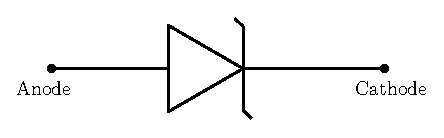
\includegraphics{chap1/fig1.44.eps}
\caption{Symbol for a zener diode}\label{fig1.44}
\end{figure}

\heading{Characteristics~:} The V-I characteristics of a zener diode is shown in Fig.~\ref{fig1.45}.
\begin{figure}[H]
\centering
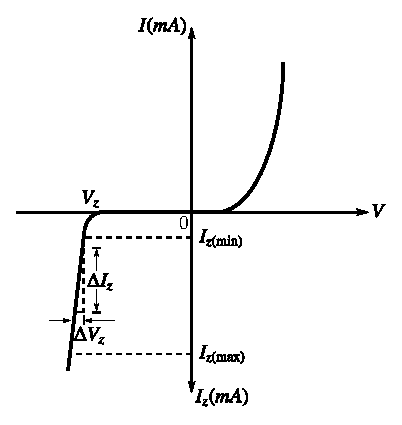
\includegraphics{chap1/fig1.45.eps}
\caption{V-I Characteristics of a Zener diode}\label{fig1.45}
\end{figure}

\eject

The forward biased characteristics of a zener diode is simply same as that of an ordinary forward biased PN junction diode. Usually zener diode is operated in reverse biased region. As we increase the reverse bias from 0 V, the current through zener diode is almost zero, till the breakdown voltage $\rmV_{\rmz}$ reaches.

When the diode is in breakdown region, the voltage across it remains almost constant (i.e., $\rmV_{\rmz}$ volts) even though the current varies through it over a wide range.

The important points on the reverse biased characteristics are
\begin{align*}
\rmV_{\rmz} &= \text{Zener breakdown voltage}\\
\rmI_{\rmZ(\min)} &= \text{the minimum zener current necessary to maintain breakdown.}\\
\rmI_{\rmZ(\max)} &= \text{the maximum zener current that is limited by the maximum power}\\
               &\quad~ \text{dissipation $\rmP_{\rmZ(\max)}$ of the diode.}
\end{align*}
\begin{equation}
\text{i.e.,}\qquad \rmP_{\rmZ(\max)}=\rmV_{\rmZ}\cdot \rmI_{\rmZ(\max)}\label{eq1.58}
\end{equation}

A very important parameter derived from the V-I characteristics is the {\em zener resistance} which is given by,
\begin{equation}
\rmr_{\rmZ}=\dfrac{\Delta \rmV_{\rmZ}}{\Delta \rmI_{\rmZ}}\Omega\label{eq1.59}
\end{equation}
Typical values of $\rmr_{\rmZ}$ range from 5 to $30\Omega$.

\subsection{Zener and Avalanche Breakdown}\label{sec1.12.1}

The breakdown in a zener diode may take place due to one of the following two mechanisms~:
\begin{itemize}
\item[(i)] Zener breakdown\qquad (ii)~ Avalanche breakdown
\end{itemize}

In a heavily doped PN junction, direct breakage of covalent bonds take place because of the strong electric field at the junction. The new electron-hole pairs so created increases the reverse current in a reverse biased PN diode. The increase in current takes place at an almost constant value of reverse bias voltage, typically below 6 V for heavily doped diodes. Due to heavy doping of P and N region, the depletion region width becomes very small and at an applied reverse bias of 6 V or less, the electric field across the depletion region becomes very high of the order of $2\times 10^{7}$Vm$^{-1}$ which is sufficient enough to break the covalent bonds. This phenomenon is called {\em Zener breakdown.}

Another breakdown process is avalanche. The phenomenon generally occurs in a wider depletion region, where the electric field is not strong enough to produce zener breakdown. Instead, minority free electrons accelerated by the electric field collide with electrons in covalent bonds. Upon collision, the covalent bonds are broken and electron-hole pairs are generated. The freed electrons are accelerated by the field, resulting in more collisions, creating more charge carriers. This process quickly results in the abrupt rise in current and this phenomenon is called {\em avalanche breakdown}.

The voltage at which breakdown occurs can be controlled in the manufacturing process since it depends on the width of the depletion region, which in turn depends on the doping level.

\section{Zener regulated power supply}\label{sec1.13}
\begin{figure}[H]
\centering
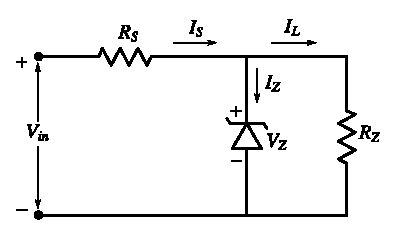
\includegraphics{chap1/fig1.46.eps}
\caption{Characteristics of a Zener diode}\label{fig1.46}
\end{figure}

Fig.~\ref{fig1.46} shows a simple circuit that maintain a constant voltage across a load resistor $\rmR_{\rmL}$. This circuit is called {\em voltage regulator}. This circuit holds the voltage across the load $\rmR_{\rmL}$ almost $\rmV_{\rmZ}$ volts, as input voltage $\rmV_{\text{in}}$ and/or load resistor $\rmR_{\rmL}$ undergo changes.

If the unregulated dc voltage $\rmV_{\text{in}}$ rises, the current through $\rmR_{\rmS}$ increases. This extra current is directed to the zener diode instead of flowing through the load. The zener diode voltage is virtually unaffected by the increase in this current and load voltage which is same as the diode voltage $\rmV_{\rmZ}$ remains almost constant.

If the load requires more current when $\rmR_{\rmL}$ is decreased, the zener diode can supply the extra current without affecting the load voltage.

From Fig.~\ref{fig1.46}, we have
\begin{align}
& \rmI_{\rmS} =\rmI_{\rmZ}+\rmI_{\rmL}\label{eq1.60}\\
& \rmI_{\rmS} =\frac{\rmV_{\text{in}}-\rmV_{\rmZ}}{\rmR_{\rmS}}\label{eq1.61}
\end{align}

The power dissipated in the zener diode is
\begin{equation}
\rmP_{\rmZ}=\rmV_{\rmZ}\cdot \rmI_{\rmZ}\label{eq1.62}
\end{equation}

The selection of $\rmR_{\rmS}$ is very important here. From \eqref{eq1.61}, we have,
\begin{equation}
\rmR_{\rmS}=\frac{\rmV_{\text{in}}-\rmV_{\rmZ}}{\rmI_{\rmS}}\label{eq1.63}
\end{equation}

Substituting Eqn.~\eqref{eq1.60} in \eqref{eq1.63}, we get
\begin{equation}
\rmR_{\rmS}=\frac{\rmV_{\text{in}}-\rmV_{\rmZ}}{\rmI_{\rmZ}+\rmI_{\rmL}}\label{eq1.64}
\end{equation}

From Fig.~\ref{fig1.46}, when $\rmR_{\rmL}$ is constant $\rmI_{\rmL}=\rmV_{\rmZ}/\rmR_{\rmL}$ is also constant. If $\rmV_{\text{in}}=\rmV_{\text{in}(\min)}$ then $\rmI_{\rmS}$ is minimum. i.e.,
\begin{align}
\rmI_{\rmS(\min)} &= \frac{\rmV_{\text{in}(\min)}-\rmV_{\rmZ}}{\rmR_{\rmS}}\label{eq1.65}\\[3pt]
\text{and}\quad \rmI_{\rmS(\min)} &= \rmI_{\rmZ(\min)}+\rmI_{\rmL}\label{eq1.66}
\end{align}

Similarly when $\rmV_{\text{in}}=\rmV_{\text{in}(\max)}$, then $\rmI_{\rmS}$ is maximum.
\begin{align}
\text{i.e.,}\quad \rmI_{\rmS(\max)} &= \frac{\rmV_{\text{in}(\max)}-\rmV_{\rmZ}}{\rmR_{\rmS}}\label{eq1.67}\\[3pt]
\text{and}\quad \rmI_{\rmS(\max)} &= \rmI_{\rmZ(\max)}+\rmI_{\rmL}\label{eq1.68}
\end{align}

The selected value of $\rmR_{\rmS}$ must be small enough to permit minimum zener current $\rmI_{\rmZ(\min)}$ to ensure that the diode is in its breakdown region. That means $\rmR_{\rmS}$ must be small enough to ensure that $\rmI_{\rmZ(\min)}$ flows under worst conditions, namely, when $\rmV_{\text{in}}$ falls to its smallest possible value $\rmV_{\text{in}(\min)}$ and $\rmI_{\rmL}$ is its largest possible value $\rmI_{\rmL(\max)}$.

$\therefore$~ From Eqn.~\eqref{eq1.64}, we get, 
\begin{equation}
\rmR_{\rmS} \leq \dfrac{\rmV_{\text{in}(\min)}-\rmV_{\rmZ}}{\rmI_{\rmZ(\min)}+\rmI_{\rmL(\max)}}\label{eq1.69}
\end{equation}

Maximum load current $\rmI_{\rmL(\max)}$ flows when load resistor $\rmR_{\rmL}$ has its minimum possible value $\rmR_{\rmL(\min)}$.
\begin{equation}
\therefore\quad \rmI_{\rmL(\max)}=\frac{\rmV_{\rmZ}}{\rmR_{\rmL(\min)}}\label{eq1.70}
\end{equation}

$\therefore$~ Substituting Eqn.~\eqref{eq1.70} in Eqn.~\eqref{eq1.69}, we get,
\begin{equation}
\rmR_{\rmS} \leq \dfrac{\rmV_{\text{in}(\min)}-\rmV_{\rmZ}}{\rmI_{\rmZ(\min)}+\frac{\rmV_{\rmZ}}{\rmR_{\rmL(\min)}}}\label{eq1.71}
\end{equation}

At the same time, the value of $\rmR_{\rmS}$ selected must be large enough to ensure that the current through the zener diode should not exceed the maximum zener current $\rmI_{\rmZ(\max)}$, so that the power dissipation in the diode will not exceed $\rmP_{\rmZ(\max)}$. That means $\rmR_{\rmS}$ must be large enough to ensure that the zener current does not exceed $\rmI_{\rmZ(\max)}$ under the worst case conditions, namely, when $\rmV_{\text{in}}$ rises to its largest possible value $\rmV_{\text{in}(\max)}$ and load current $\rmI_{\rmL}$ to its minimum value $\rmI_{\rmL(\min)}$.

$\therefore$~ From Eqn.~\eqref{eq1.64}, we get
\begin{equation}
\rmR_{\rmS}\geq \frac{\rmV_{\text{in}(\max)}-\rmV_{\rmZ}}{\rmI_{\rmZ(\max)}+\rmI_{\rmL(\min)}}\label{eq1.72}
\end{equation}

Minimum load current $\rmI_{\rmL(\min)}$ flows, when load resistor $\rmR_{\rmL}$ has its maximum possible value $\rmR_{\rmL(\max)}$.
\begin{equation}
\text{i.e.,}\quad \rmI_{\rmL(\min)}=\frac{\rmV_{\rmZ}}{\rmR_{\rmL(\max)}}\label{eq1.73}
\end{equation}

Substituting Eqn.~\eqref{eq1.73} in Eqn.~\eqref{eq1.72}, we get,
\begin{equation}
\rmR_{\rmS}\geq \frac{\rmV_{\text{in}(\max)}-\rmV_{\rmZ}}{\rmI_{\rmZ(\max)}+\frac{\rmV_{\rmZ}}{\rmR_{\rmL(\max)}}}\label{eq1.74}
\end{equation}

\medskip
\begin{center}
\rule{4cm}{1pt}\\
{\bf\Large Problems}\\[-3pt]
\rule{4cm}{1pt}
\end{center}

\begin{problem}\label{prob1.27}
In a zener voltage regulator if $\rmV_{\rmZ}=10\rmV$, $\rmR_{\rmS}=1\rmk\Omega$, $\rmR_{\rmL}=2\rmk\Omega$. If the input voltage $\rmV_{\text{in}}$ varies from 22 to 40 V, find the maximum and minimum values of zener current.
\end{problem}

\begin{solution}
Given~ $\rmV_{\rmZ}=10\rmV$, \ $\rmR_{\rmS}=1\rmk\Omega$,  \ $\rmR_{\rmL}=2\rmk\Omega$,
$$
\rmV_{\text{in}(\min)}=22\rmV,\quad \rmV_{\text{in}(\max)}=40\rmV.
$$
We have
\begin{align*}
\rmI_{\rmL} &= \frac{\rmV_{\rmZ}}{\rmR_{\rmL}}=\frac{10}{2\times 10^{3}}=5\text{~mA}\\[3pt]
\rmI_{\rmS} &= \frac{\rmV_{\text{in}}-\rmV_{\rmZ}}{\rmR_{\rmS}}\\[3pt]
\rmI_{\rmS(\min)} &= \frac{\rmV_{\text{in}(\min)}-\rmV_{\rmZ}}{\rmR_{\rmS}}\\[3pt]
&= \frac{22-10}{1\times 10^{3}}\\[3pt]
\therefore\quad \rmI_{\rmS(\min)} &= 12\text{~mA}.\\[3pt]
\text{Also we have~~ } \rmI_{\rmS} &= \rmI_{\rmZ}+\rmI_{\rmL}\\[3pt]
\therefore\quad \rmI_{\rmZ(\min)} &= \rmI_{\rmS(\min)}-\rmI_{\rmL}\\[3pt]
&= 12\times 10^{-3}-5\times 10^{-3}\\
&= 7\text{~mA}\\[3pt]
\text{Similarly}\quad \rmI_{\rmS(\max)} &= \frac{\rmV_{\text{in}(\max)}-\rmV_{\rmZ}}{\rmR_{\rmS}}=\dfrac{40-10}{1\times 10^{3}}\\[3pt]
\therefore\quad \rmI_{\rmS(\max)} &= 30\text{~mA}\\[3pt]
\rmI_{\rmS(\max)} &= \rmI_{\rmZ(\max)}+\rmI_{\rmL}\\[3pt]
\therefore\quad \rmI_{\rmZ(\max)} &= \rmI_{\rmS(\max)}-\rmI_{\rmL}\\[3pt]
&= 30\times 10^{-3}-5\times 10^{-3}\\[3pt]
\rmI_{\rmZ(\max)} &= 25\text{~mA}
\end{align*}
\begin{align*}
\therefore\quad \text{Minimum zener current~~ } \rmI_{\rmZ(\min)} &= 7\text{~mA}\\[3pt]
\text{and maximum zener current~~ } \rmI_{\rmZ(\max)} &= 25\text{~mA}
\end{align*}
\end{solution}

\begin{problem}\label{prob1.28}
The zener diode in Fig.~\ref{fig1.47} has breakdown voltage of 10 V. What are the minimum and maximum zener current ?
\begin{figure}[H]
\centering
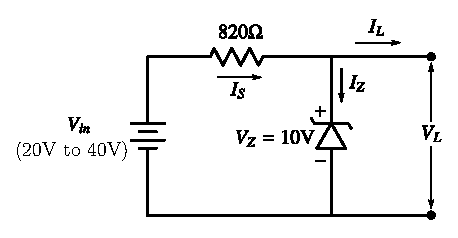
\includegraphics{chap1/fig1.47.eps}
\caption{}\label{fig1.47}
\end{figure}
\end{problem}

\begin{solution}
Given~~ $\rmV_{\text{in}(\min)}=20\rmV$, \ $\rmV_{\text{in}(\max)}=40\rmV$,
$$
\rmV_{\rmZ}=10\text{~V}, \ \ \rmR_{\rmS}=820\,\Omega, \ \ \rmR_{\rmL}=\infty.
$$

Since $\rmR_{\rmL}=\infty$, \ $\rmI_{\rmL}=0$.

\eject

We have
\begin{align*}
\rmI_{\rmS} &= \rmI_{\rmS}+\rmI_{\rmL}\\[3pt]
\rmI_{\rmS} &= \rmI_{\rmZ}\qquad [\because \ \rmI_{\rmL}=0]\\[3pt]
\therefore\quad \rmI_{\rmS(\max)} &= \frac{\rmV_{\text{in}(\max)}-\rmV_{\rmZ}}{\rmR_{\rmS}}= \frac{40-10}{820}\\[3pt]
\rmI_{\rmS(\max)} &= 36.6\text{~mA}\\[3pt]
\therefore\quad \rmI_{\rmZ(\max)} &= 36.6\text{~mA}\\[3pt]
\rmI_{\rmS(\min)} &= \frac{\rmV_{\text{in}(\min)}-\rmV_{\rmZ}}{\rmR_{\rmS}}
= \frac{20-10}{820}\\[3pt]
\rmI_{\rmS(\min)} &= 12.2\text{~mA}\\[3pt]
\therefore\quad \rmI_{\rmZ(\min)} &= 12.2\text{~mA}
\end{align*}
\begin{align*}
\text{Maximum zener current~~ } \rmI_{\rmZ(\max)} &= 36.6\text{~mA}\\[3pt]
\text{Minimum zener current~~ } \rmI_{\rmZ(\min)} &= 12.2\text{~mA}
\end{align*}
\end{solution}

\begin{problem}\label{prob1.29}
In the circuit shown in Fig.~\ref{fig1.48}, determine
\begin{itemize}
\item[(a)] the load current

\item[(b)] the zener current

\item[(c)] power dissipated in resistor $\rmR_{\rmS}$

\item[(d)] power dissipated in load resistor $\rmR_{\rmL}$

\item[(e)] power dissipated in zener diode
\end{itemize}
\begin{figure}[H]
\centering
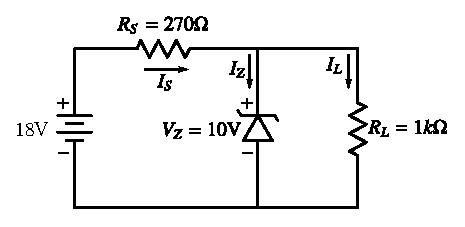
\includegraphics{chap1/fig1.48.eps}
\caption{}\label{fig1.48}
\end{figure}
\end{problem}

\begin{solution}
Given
\begin{align*}
\rmV_{\text{in}} &= 18\rmV, \ \ \rmR_{\rmS}=270\Omega\\[4pt]
\rmV_{\rmZ} &= 10\rmV, \ \ \rmR_{\rmL}=1\rmk\Omega\\[4pt]
\text{Source Current~~ } \rmI_{\rmS} &= \dfrac{\rmV_{\text{in}}-\rmV_{\rmZ}}{\rmR_{\rmS}}\\[4pt]
&= \frac{18-10}{270}\\[4pt]
\rmI_{\rmS} &= 29.62\text{~mA}
\end{align*}
\begin{itemize}
\item[(a)] Load current \ \ $\rmI_{\rmL}=\dfrac{\rmV_{\rmZ}}{\rmR_{\rmL}}=\dfrac{10}{1\times 10^{3}}=10\text{~mA}$

\item[(b)] We have\quad $\rmI_{\rmS}=\rmI_{\rmZ}+\rmI_{\rmL}$
\begin{align*}
\therefore~ \text{~ Zener current}\quad \rmI_{\rmZ} &= \rmI_{\rmS}-\rmI_{\rmL}\\[4pt]
          &= 29.62\times 10^{-3}-10\times 10^{-3}\\[4pt]
          &= 19.62\text{~mA}
\end{align*}

\item[(c)] 
\begin{tabbing}
Power dissipitated in resistor $\rmR_{\rmS}$ \== $\rmI_{\rmS}^{2}\cdot \rmR_{\rmS}$\\[6pt]
          \>= $(29.62\times 10^{-3})^{2}\times 270$\\[6pt]
          \>= $236.9\text{~mW}$
\end{tabbing}

\item[(d)]
\begin{tabbing}
Power dissipated in zener diode~~ $\rmP_{\rmZ}$ \== $\rmV_{\rmZ}\cdot \rmI_{\rmZ}$\\[6pt]
    \>= $10\times 19.62\times 10^{-3}$\\[6pt]
    \>= $196.2$~ mW
\end{tabbing}

\item[(e)]
\begin{tabbing}
Power dissipated in load resistor~~ $\rmR_{\rmL}$ \== $\rmI_{\rmL}^{2}\cdot \rmR_{\rmL}$\\[6pt]
 \>= $(10\times 10^{-3})^{2}\times 1\times 10^{3}$\\[6pt]
 \>= 100 mW
\end{tabbing}
\end{itemize}
\end{solution}

\eject

\begin{problem}\label{prob1.30}
Design a zener voltage regulator for the following specifications. Output voltage = 5V, input voltage $\rmV_{\text{in}}=(12\pm 3)\rmV$, load current $\rmI_{\rmL}=20$~mA, Zener wattage $\rmP_{\rmZ(\max)}=500$ mW, $\rmI_{\rmZ(\min)}=2$~mA.
\end{problem}

\begin{solution}
Given, $\rmV_{\rmZ}=5\rmV$, \ $\rmI_{\rmL}=20$~mA, \ $\rmP_{\rmZ(\max)}=500$~mW, \ $\rmI_{\rmZ(\min)}=2$~mA, \ $\rmV_{\text{in}(\min)}=12-3=9\rmV$, \ $\rmV_{\text{in}(\max)}=12+3=15\rmV$.

\vskip .1cm
Load resistor \ \ $\rmR_{\rmL}=\dfrac{\rmV_{\rmL}}{\rmI_{\rmL}}=\dfrac{\rmV_{\rmZ}}{\rmI_{\rmL}}=\dfrac{5}{20\times 10^{-3}}=250\Omega$

\vskip .1cm
Maximum zener wattage $\rmP_{\rmZ(\max)}=500$~mW

\vskip .1cm
We have\quad $\rmP_{\rmZ(\max)}=\rmV_{\rmZ}\cdot \rmI_{\rmZ(\max)}$

\vskip .1cm
$\therefore$~ Maximum allowed zener current
\begin{align*}
\rmI_{\rmZ(\max)} &= \dfrac{\rmP_{\rmZ(\max)}}{\rmV_{\rmZ}}\\[4pt]
               &= \frac{500\times 10^{-3}}{5}\\[4pt]
\rmI_{\rmZ(\max)} &= 100\text{~mA}
\end{align*}
We have\quad $\rmR_{\rmS}=\dfrac{\rmV_{\text{in}}-\rmV_{\rmZ}}{\rmI_{\rmZ}}=\dfrac{\rmV_{\text{in}}-\rmV_{\rmZ}}{\rmI_{\rmZ}+\rmI_{\rmL}}$

\vskip .25cm
Here, $\rmI_{\rmL}=20$~mA constant
\begin{align*}
\rmR_{\rmS} &\leq \dfrac{\rmV_{\text{in}(\min)}-\rmV_{\rmZ}}{\rmI_{\rmZ(\min)}+\rmI_{\rmL}}\\[4pt]
           &\leq \dfrac{9-5}{2\times 10^{-3}+20\times 10^{-3}}\\[4pt]
\rmR_{\rmS} &\leq 181.8\Omega
\end{align*}

At the same time
\begin{align*}
\rmR_{\rmS} &\geq \dfrac{\rmV_{\text{in}(\max)}-\rmV_{\rmZ}}{\rmI_{\rmZ(\max)}+\rmI_{\rmL}}\\[4pt]
          &\geq \dfrac{15-5}{100\times 10^{-3}+20\times 10^{-3}}\\[4pt]
\rmR_{\rmS} &\geq 83.3\Omega
\end{align*}
$\therefore$~ $83.3\Omega\leq \rmR_{\rmS}\leq 181.8\Omega$

\noindent
$\therefore$~ Select $\rmR_{S}=120\,\Omega$ (say)

The circuit diagram is shown in Fig.~\ref{fig1.49}
\begin{figure}[H]
\centering
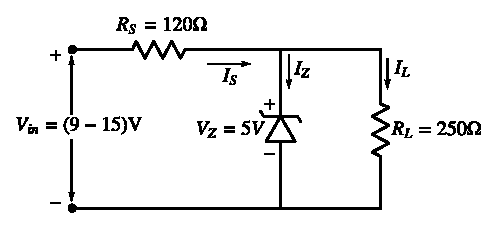
\includegraphics{chap1/fig1.49.eps}
\caption{}\label{fig1.49}
\end{figure}
\end{solution}

\begin{problem}\label{prob1.31}
The zener diode in a regulator circuit has a breakdown voltage of $15\rmV$ and power rating of 0.5\,W. If $\rmV_{\text{in}}=40\rmV$, what is minimum value of $\rmR_{\rmS}$ that prevents zener diode from being destroyed ?
\end{problem}

\begin{solution}
Given~:~ $\rmV_{\rmZ}=15\rmV$, \ $\rmP_{\rmZ(\max)}=0.5\rmW$, \ $\rmV_{\text{in}}=40\rmV$

Maximum allowable zener current
\begin{align*}
\rmI_{\rmZ(\max)} &= \frac{\rmP_{\rmZ(\max)}}{\rmV_{\rmZ}}\\[4pt]
&= \frac{0.5}{15}\\[4pt]
\rmI_{\rmZ(\max)} &= 33.33\text{~mA}
\end{align*}

Maximum current through zener diode flows when either $\rmV_{\text{in}}$ is maximum or $\rmR_{\rmL}$ is maximum. But here $\rmV_{\text{in}}=40\rmV$ is constant and $\rmR_{\rmL(\max)}=\infty$ (i.e. open circuit).

Then 
$$
\rmI_{\rmL(\min)}=\rmV_{\rmZ}/\rmR_{\rmL(\max)}=0
$$

We have
\begin{align*}
\rmR_{\rmS} &= \dfrac{\rmV_{\text{in}}-\rmV_{\rmZ}}{\rmI_{\rmZ}+\rmI_{\rmL}}\\[4pt]
\therefore\quad \rmR_{\rmS} &\geq \dfrac{\rmV_{\text{in}}-\rmV_{\rmZ}}{\rmI_{\rmZ(\max)}+\rmI_{\rmL(\min)}}\\[4pt]
&\geq \dfrac{40-15}{33.33\times 10^{-3}+0}\\[4pt]
\therefore\quad \rmR_{\rmS} &\geq 750.1\Omega
\end{align*}
$\therefore$~ Minimum value of required $\rmR_{\rmS}\simeq 750.1\Omega$.
\end{solution}

\begin{problem}\label{prob1.32}
In the circuit shown in Fig.~\ref{fig1.50}, the desired load voltage $\rmV_{\rmL}=10\rmV$. A $10\rmV$ zener diode is used, which has a maximum power dissipation rating of $50\rmW$ and needs a minimum current of 10\,mA to ensure that it operates in the breakdown region. Determine the range of values of $\rmR_{\rmS}$.
\begin{figure}[H]
\centering
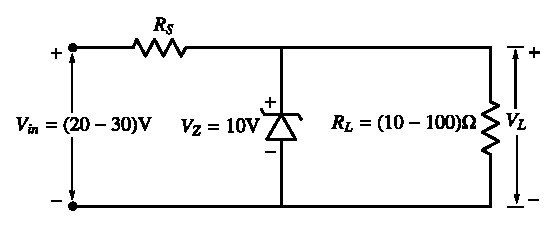
\includegraphics{chap1/fig1.50.eps}
\caption{}\label{fig1.50}
\end{figure}
\end{problem}

\begin{solution}
Given~:
\begin{align*}
& \rmV_{\text{in}(\min)}=20\rmV, \ \rmR_{\rmL(\min)}=10\Omega, \ \rmV_{\text{in}(\max)}=30\rmV, \ \rmR_{\rmL(\max)}=100\Omega,\\[4pt]
& \rmV_{\rmL}=\rmV_{\rmZ}=10\rmV, \ \rmI_{\rmZ(\min)}=10\text{~mA}, \ \rmP_{\rmZ(\max)}=50\rmW
\end{align*}
The maximum allowable zener current
\begin{align*}
\rmI_{\rmZ(\max)} &= \frac{\rmP_{\rmZ(\max)}}{\rmV_{\rmZ}}= \frac{50}{10}= 5\rmA
\end{align*}
We have
\begin{align*}
\rmR_{\rmS} &= \frac{\rmV_{\text{in}}-\rmV_{\rmZ}}{\rmI_{\rmZ}+\rmI_{\rmL}}\\[4pt]
\therefore\quad \rmR_{\rmS} &= \frac{\rmV_{\text{in}}-\rmV_{\rmZ}}{\rmI_{\rmZ}+\frac{\rmV_{\rmZ}}{\rmR_{\rmL}}}
\end{align*}

We have,
\begin{align*}
\rmR_{\rmS} &\leq \dfrac{\rmV_{\text{in}(\min)}-\rmV_{\rmZ}}{\rmI_{\rmZ(\min)}+\frac{\rmV_{\rmZ}}{\rmR_{\rmL(\min)}}}\\[4pt]
&\leq \dfrac{20-10}{10\times 10^{-3}+\frac{10}{10}}\\[4pt]
\rmR_{\rmS} &\leq 9.9\Omega
\end{align*}
Also we have,
\begin{align*}
\rmR_{\rmS} &\geq \dfrac{\rmV_{\text{in}(\max)}-\rmV_{\rmZ}}{\rmI_{\rmZ(\max)}+\frac{\rmV_{\rmZ}}{\rmR_{\rmL(\max)}}}\\[4pt]
&\geq \dfrac{30-10}{5+\frac{10}{100}}\\[4pt]
\therefore\quad \rmR_{\rmS} &\geq 3.92\Omega
\end{align*}
$\therefore~ 3.92\Omega\leq \rmR_{\rmS}\leq 9.9\Omega$.
\end{solution}

\begin{problem}\label{prob1.33}
For the circuit shown below in Fig.~\ref{fig1.51}, $\rmV_{\rmL}=15\rmV$, maximum load current is 100~mA, minimum load current is 0~A, minimum load current is 0~A, input voltage range is 18V to 20V, $\rmR_{\rmS}=10\Omega$. Determine,
\begin{itemize}
\item[(a)] maximum power dissipated by $\rmR_{\rmS}$

\item[(b)] minimum diode current

\item[(c)] the power that must be dissipated by $\rmR_{\rmS}$ if the output is accidentally short circuited.
\begin{figure}[H]
\centering
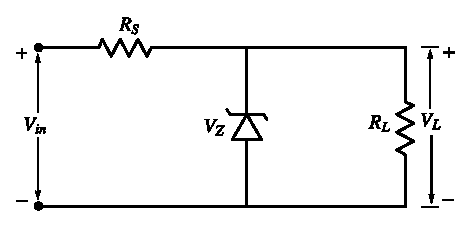
\includegraphics{chap1/fig1.51.eps}
\caption{}\label{fig1.51}
\end{figure}
\end{itemize}
\end{problem}

\begin{solution}
Given~:~ $\rmV_{\text{in}(\max)}=20\rmV$, \ $\rmV_{\text{in}(\min)}=18\rmV$, \ $\rmI_{\rmL(\max)}=100\text{~mA}$, $\rmI_{\rmL(\min)}=0\rmA$, \ $\rmR_{\rmS}=10\Omega$, \ $\rmV_{\rmL}=\rmV_{\rmZ}=15\rmV$
\begin{itemize}
\item[(a)] $\rmI_{\rmS}$ is maximum when $\rmV_{\text{in}}$ is maximum
\begin{align*}
\therefore\quad \rmI_{\rmS(\max)} &= \dfrac{\rmV_{\text{in}(\max)}-\rmV_{\rmZ}}{\rmR_{\rmS}}\\[4pt]
&= \dfrac{20-15}{10}\\[4pt]
\rmI_{\rmS(\max)} &= 500\text{~mA}
\end{align*}
$\therefore$~ Maximum power dissipated by
\begin{align*}
\rmR_{\rmS} &= \rmI^{2}_{\rmS(\max)}\cdot \rmR_{\rms}\\[4pt]
&= (500\times 10^{-3})^{2}\times 10\\[4pt]
&= 2.5\rmW
\end{align*}

\item[(b)] Diode current is minimum when $\rmV_{\text{in}}$ is minimum and $\rmI_{\rmL}$ is maximum 

We have
\begin{align*}
\rmI_{\rmS(\min)} &= \dfrac{\rmV_{\text{in}(\min)}-\rmV_{\rmZ}}{\rmR_{\rmS}}\\[4pt]
&= \frac{18-15}{10}\\[4pt]
\rmI_{\rmS(\min)} &= 300\text{~mA}
\end{align*}
Also \ $\rmI_{\rmS}=\rmI_{\rmZ}+\rmI_{\rmL}$
\begin{align*}
\therefore\quad \rmI_{\rmS(\min)} &= \rmI_{\rmZ(\min)}+\rmI_{\rmL(\max)}\\[4pt]
\therefore\quad \rmI_{\rmZ(\min)} &= \rmI_{\rmS(\min)}-\rmI_{\rmL(\max)}\\[4pt]
&= 300\times 10^{-3}-100\times 10^{-3}\\[3pt]
\therefore\quad \rmI_{\rmZ(\min)} &= 200\text{~mA}
\end{align*}

\item[(c)] When the output is short circuited i.e., when $\rmR_{\rmL}$ becomes zero
\begin{align*}
\rmI_{\rmS(\max)}=\rmI_{\rmL} &= \frac{\rmV_{\text{in}(\max)}}{\rmR_{\rmS}}\qquad [\because \ \rmI_{\rmZ}\text{~~ becomes zero}]\\[4pt]
&= \dfrac{20}{10}\\[4pt]
&= 2\rmA
\end{align*}
$\therefore$~ the power that must be dissipated by $\rmR_{\rmS}$
\begin{align*}
&= \rmI^{2}_{\rmS(\max)}\cdot \rmR_{\rmS}\\[4pt]
&= 2^{2}\times 10\\[4pt]
&= 40\rmW
\end{align*}
\end{itemize}
\end{solution}

\heading{Practical zener diode~:} Ideally zener diode has resistance of zero ohms in the breakdown region. In this case, the zener diode with breakdown voltage $\rmV_{\rmZ}$ may be represented by a voltage source $\rmV_{\rmZ}$ as shown in Fig.~\ref{fig1.52} below.
\begin{figure}[H]
\centering
\includegraphics{chap1/fig1.52.eps}
\caption{Equivalent circuit of an ideal zener diode}\label{fig1.52}
\end{figure}

But practically, zener diode has a small resistance $\rmr_{\rmz}$ (usually 5 to $30\Omega$) in the breakdown region. In this case, the zener diode with breakdown voltage $\rmV_{\rmz}$ and resistance $\rmr_{\rmz}$ may be represented by a voltage source $\rmV_{\rmz}$ in series the resistance $\rmr_{\rmz}$, as shown in Fig.~\ref{fig1.53}.
\begin{figure}[H]
\centering
\includegraphics{chap1/fig1.53.eps}
\caption{Equivalent circuit of a practical zener diode}\label{fig1.53}
\end{figure}

Practically, the total voltage drop across a zener diode in breakdown region is 
\begin{equation}
\rmV=\rmV_{\rmZ}+\rmI_{\rmZ}\cdot \rmr_{\rmZ}
\end{equation}
where $\rmI_{\rmz}$ = current through zener diode.

\begin{problem}\label{prob1.34}
In the voltage regulating circuit shown in Fig.~\ref{fig1.54},
\begin{itemize}
\item[(a)] Find the load voltage $\rmV_{\rmL}$.

\item[(b)] If $\rmV_{\rmL}$ incrases by 1\%\ while $\rmI_{\rmL}$ remains at 50 mA, what is the corresponding value of $\rmV_{\text{in}}$~?

\eject

\item[(c)] What is the power consumption of the zener diode under the condition in part (b) ?
\begin{figure}[H]
\centering
\includegraphics{chap1/fig1.54.eps}
\caption{}\label{fig1.54}
\end{figure}
\end{itemize}
\end{problem}

\begin{solution}
Given~:
\begin{align*}
& \rmV_{\rmZ} =\rmV_{\rmL}=100\rmV, \ \rmr_{\rmZ}=25\Omega, \ \rmR_{\rmS}=250\Omega,\\[5pt]
& \rmI_{\rmZ}=10\text{~mA}, \ \rmI_{\rmL}=50\text{~mA}
\end{align*}

The above circuit in Fig.~\ref{fig1.54} is redrawn in Fig.~\ref{fig1.55} with zener diode replaced by its equivalent circuit.
\begin{figure}[H]
\centering
\includegraphics{chap1/fig1.55.eps}
\caption{}\label{fig1.55}
\end{figure}
\begin{itemize}
\item[(a)] Load voltage
\begin{align*}
\rmV_{\rmL} &= \rmV_{\rmZ}+\rmI_{\rmZ}\rmr_{\rmZ}\\[4pt]
          &= 100+10\times 10^{-3}\times 25\\[4pt]
\rmV_{\rmL} &= 100.25\rmV
\end{align*}

\eject

Input voltage
\begin{align*}
\rmV_{\text{in}} &= \rmV_{\rmL}+\text{~voltage drop across } \rmR_{\rmS}\\[4pt]
&= \rmV_{\rmL}+\rmI_{\rmS}\cdot \rmR_{\rmS}\\[4pt]
&= \rmV_{\rmL}+(\rmI_{\rmZ}+\rmI_{\rmL})\cdot \rmR_{\rmS}\\[4pt]
&= 100.25+(10\times 10^{-3}+50\times 10^{-3})\times 250\\[4pt]
\therefore\quad \rmV_{\text{in}} &= 115.25\rmV
\end{align*}

\item[(b)] If the load voltage increased by 1\%, the new value is $\rmV^{1}_{\rmL}=1\%$ of $\rmV_{\rmL}$
\begin{align*}
&= 1.01\times 100.25\\[4pt]
\rmV_{\rmL}^{1} &= 101.25\rmV\\[4pt]
\text{We have}\quad \rmV_{\rmL}^{1} &= \rmV_{\rmZ}+\rmI^{1}_{\rmZ}\cdot \rmr_{\rmZ}
\end{align*}

\begin{tabbing}
Then the corresponding value of zener current \ $\rmI^{1}_{\rmZ}$ \== $\dfrac{\rmV^{1}_{\rmL}-\rmV_{\rmZ}}{\rmr_{\rmZ}}$\\[5pt]
\>= $\dfrac{101.25-100}{25}$\\[4pt]
\>= 50~mA
\end{tabbing}

\begin{tabbing}
Then the corresponding input voltage \ $\rmV_{\text{in}}^{1}$ \== $\rmV^{1}_{\rmL}+(\rmI^{1}_{\rmZ}+\rmI_{\rmL})\rmR_{\rmS}$\\[5pt]
\>= $101.25+(50\times 10^{-3}+50\times 10^{-3})\times 250$\\[5pt]
$\rmV^{1}_{\text{in}}$ \>= $126.25\rmV$
\end{tabbing}

\item[(c)] The power consumed by zener diode
\begin{align*}
\rmP_{\rmZ} &= \rmV_{\rmZ}\rmI^{1}_{\rmZ}\\[5pt]
&= 100\times 50\times 10^{-3}\\[5pt]
\rmP_{\rmZ} &= 5\rmW
\end{align*}
\end{itemize}
\end{solution}

\eject

\begin{center}
\rule{4cm}{1pt}\\
{\bf\Large Exercises}\\[-3pt]
\rule{4cm}{1pt}
\end{center}

\begin{enumerate}
\renewcommand{\labelenumi}{(\theenumi)}
\item The forward current in a PN junction is 5 mA at $20^{\circ}$C. If reverse saturation current is $5.5\times 10^{-7}$A and $\eta=1$, what is the forward biasing voltage across the junction ?

\noindent
{\bf Ans~:} $V\simeq 0.24\rmV$.

\item A germanium diode carries a current of 15 mA when a forward bias of 0.18 V is applied across it at $27^{\circ}$C (Given $\eta=1$).
\begin{itemize}
\item[(a)] Find the reverse saturation current.

\item[(b)] Calculate the bias voltage needed for diode current of 50~mA.
\end{itemize}

\noindent
{\bf Ans~:}~ (a)~ $\rmI_{\rmo}\simeq 14.7\mu\rmA$\qquad (b)~ $\rmV=0.21\rmV$.

\item A Si PN junction is formed from p-material doped with $2\times 10^{22}$ acceptors/m$^{3}$ and n-material doped with $1.8\times 10^{22}$ donors/m$^{3}$. Find the thermal voltage and barrier voltage at $27^{\circ}$C.

Given that $\rmn_{\rmi}=1.5\times 10^{16}$ carriers/m$^{3}$ for Si at $27^{\circ}$C.

\smallskip
\noindent
{\bf Ans~:}~ $\rmV_{\rmT}\simeq 26\text{~mV}$, \ $\rmV_{\rmo}=0.73\rmV$.

\item Find the factor by which the reverse saturation current of a silicon diode is multiplied when the temperature is increased from $35^{\circ}$C to $125^{\circ}$C.

\smallskip
\noindent
{\bf Ans~:} 512.

\item A germanium PN junction diode has a reverse saturation current of 50$\mu$A at a temperature of $35^{\circ}$C. Find the reverse saturation current at $90^{\circ}$C.

\smallskip
\noindent
{\bf Ans~:} $\rmI_{\rmo}(\rmT)\simeq 2263\mu \rmA$.

\item A silicon diode has a reverse saturation current of 0.18 $\mu$A at $30^{\circ}$C. (a) Find its current when it is forward biased by 0.65 V. (b) Find the current in the same diode when the temperature rises to $75^{\circ}$C.

Given that for Si : $\eta=2$.

\smallskip
\noindent
{\bf Ans~:} (a)~ 44.9 mA\qquad (b)~ 203.6 mA.

\item A sinusoidal voltage of peak value 65 V and frequency 50 Hz is applied to a half-wave rectifier. No filter is used. The load resistor is 1000 $\Omega$. Neglect cut-in voltage. Consider $\rmR_{\rmf}=10\Omega$ and $\rmR_{\rmr}=\infty$. Calculate,
\begin{itemize}
\item[(a)] peak, dc and rms values of current.

\item[(b)] dc output power.

\item[(c)] ac input power.

\item[(d)] rectifier efficiency.
\end{itemize}
\begin{description}
\item[{\bf Ans~:}] (a) $\rmI_{\rmm}=64.36$~mA; \ $\rmI_{\text{de}}=20.5$~mA; \ $\rmI_{\text{rms}}=32.18$~mA

(b)~ $\rmP_{\text{de}}=420.25$~mW; \ (c)~ $\rmP_{\text{ac}}\simeq 1046$~mW; \ (d)~ $\eta=40.18\%$.
\end{description}

\item What peak-to-peak sinusoidal voltage must be connected to a half-wave rectifier if the rectified waveform is to have a dc value of 10 V? Assume that the forward drop across the diode is 0.6 V.

\smallskip
\noindent
{\bf Ans~:}~ 66.6\,V.

\item A full-wave rectifier supplies a load of 1 k$\Omega$. The ac voltage applied to the diode is 280-0-280 V. If the diode forward resistance is neglected, calculate, 
\begin{itemize}
\item[(a)] dc output current.

\item[(b)] dc output voltage.

\item[(c)] ripple voltage.
\end{itemize}

\smallskip
\noindent
{\bf Ans~:}~ (a)~ $\rmI_{\text{dc}}\simeq 252$ mA\qquad (b)~ $\rmV_{\text{dc}}=252\rmV$\qquad (c)~ $\rmV_{\text{r,rms}}\simeq 121\rmV$.

\item A sinusoidal voltage of $330\sin 314\rmt$ V is applied to a full-wave bridge rectifier. Determine the dc load current, dc load voltage and efficiency, if $\rmR_{\rmL}=10\rmk\Omega$. Assume $\rmR_{\rmf}=8\Omega$.

\smallskip
\noindent
{\bf Ans~:~} $\rmI_{\text{dc}}=20.98$\,mA;\quad $\rmV_{\text{dc}}=210\,\rmV$;\quad $\eta=80.9\%$

\item A half-wave rectifier using a capacitor filter is to supply 100 $\rmV_{\text{dc}}$ to a 10 k$\Omega$ load. Assuming the diode forward resistance is negligible, calculate the input voltage required and the value of filter capacitor for a ripple factor of 0.05. Given that power line frequency $f=50$~Hz.

\smallskip
\noindent
{\bf Ans~:}~ 76.8 V;\quad $\rmC$ = greater than 11.55 $\mu\rmF$.

\item A 230 V, 50 Hz input is applied to a bridge rectifier with load 1 k$\Omega$. Calculate the output dc voltage, dc load current and ripple factor.
\begin{itemize}
\item[(a)] without capacitor filter.

\item[(b)] with capacitor filter $\rmC=500~\mu\rmF$. 
\end{itemize}
Assume diodes are ideal.
\begin{description}
\item[{\bf Ans~:}] (a)~ $\rmV_{\text{dc}}\simeq 207\rmV$;\quad $\rmI_{\text{dc}}=207.1~\text{mA}$;\quad $\rmr=0.483$

(b)~ $\rmV_{\text{dc}}\simeq 322\rmV$;\quad $\rmI_{\text{dc}}=322~\text{mA}$;\quad $\rmr=0.0058$ 
\end{description}

\item Consider a bridge rectifier circuit with capacitor filter which has transformer ratio $5:1$, $\rmR_{\rmL}=1\rmk\Omega$ and $\rmC=500\rmu\rmF$. If the rms input voltage to the transformer primary is 150 V, 50 Hz, determine,
\begin{itemize}
\item[(a)] rms ripple voltage.

\item[(b)] dc load voltage.

\item[(c)] dc load power.
\end{itemize}

\noindent
{\bf Ans~:}~ $0.2\rmV$\quad (b)~ $42\rmV$\quad (c)~ $1.76\rmW$.

\item A load is to be supplied 50 mA at 110 $\rmV_{\text{dc}}$ with a ripple not more than 1.5\%. Calculate the value of the filter capacitor that would be needed for a full wave bridge rectifier circuit. Main source voltage is 200 V, 50 Hz. Also calculate transformer turn ratio.

\smallskip
\noindent
{\bf Ans~:~} $\rmC>87.5\,\mu\rmF$; \ \ Select $\rmC=90\,\mu\rmF$

$\rmN_{1}:\rmN_{2}=2.8:1$

\item In the circuit shown in Fig.~\ref{fig1.56} below, determine
\begin{itemize}
\item[(a)] the load current

\item[(b)] the zener current

\item[(c)] power dissipated in resistor $\rmR_{\rmS}$

\item[(d)] power dissipated in load resistor $\rmR_{\rmL}$

\item[(e)] power dissipated in zener diode
\end{itemize}
\begin{figure}[H]
\centering
\includegraphics{chap1/fig1.56.eps}
\caption{}\label{fig1.56}
\end{figure}

\noindent
{\bf Ans~:~} (a)~ 7.27\,mA\quad (b)~ 11.88\,mA\quad (c)~ 172.36\,mW\quad (d)~ 116.28\,mW\quad (e)~ 190.1\,mW.
\end{enumerate}

\label{1end}
